%% LyX 2.1.4 created this file.  For more info, see http://www.lyx.org/.
%% Do not edit unless you really know what you are doing.
\documentclass[oneside,american,spanish,english]{book}
\usepackage[T1]{fontenc}
\usepackage[utf8]{luainputenc}
\setcounter{secnumdepth}{3}
\setcounter{tocdepth}{3}
\usepackage{color}
\usepackage{float}
\usepackage{calc}
\usepackage{graphicx}
\usepackage[numbers]{natbib}
\usepackage{subscript}

\makeatletter

%%%%%%%%%%%%%%%%%%%%%%%%%%%%%% LyX specific LaTeX commands.
%% Because html converters don't know tabularnewline
\providecommand{\tabularnewline}{\\}

%%%%%%%%%%%%%%%%%%%%%%%%%%%%%% Textclass specific LaTeX commands.
\newenvironment{lyxlist}[1]
{\begin{list}{}
{\settowidth{\labelwidth}{#1}
 \setlength{\leftmargin}{\labelwidth}
 \addtolength{\leftmargin}{\labelsep}
 \renewcommand{\makelabel}[1]{##1\hfil}}}
{\end{list}}

%%%%%%%%%%%%%%%%%%%%%%%%%%%%%% User specified LaTeX commands.
\usepackage{multirow}
\usepackage{multicol} 
\usepackage{colortbl}
\usepackage[printonlyused]{acronym}
\usepackage{pslatex}
\usepackage{txfonts}
\usepackage[small,bf]{caption}
\usepackage{acronym}
\usepackage{mathpazo}
\usepackage{listings}
\usepackage{algorithm}
\usepackage{algpseudocode}
\usepackage[Lenny]{fncychap}
\usepackage{fancyhdr}
\usepackage{graphicx}
\lstloadlanguages{Java}
\restylefloat{algorithm}
\floatstyle{plain}
\definecolor{gray}{gray}{0.7}

\makeatother

\usepackage{babel}
\addto\shorthandsspanish{\spanishdeactivate{~<>}}

\usepackage{listings}
\addto\captionsamerican{\renewcommand{\lstlistingname}{Listing}}
\addto\captionsenglish{\renewcommand{\lstlistingname}{Listing}}
\addto\captionsspanish{\renewcommand{\lstlistingname}{Listado de código}}
\renewcommand{\lstlistingname}{Listing}

\begin{document}
\thispagestyle{empty}

\selectlanguage{spanish}%
\begin{center}
Universidad Nacional del Centro de la Provincia De Buenos Aires\\
Facultad de Ciencias Exactas - Departamento de Computación y Sistemas\\
Ingeniería de Sistemas
\par\end{center}

\begin{center}

\includegraphics[scale=0.6]{images/unicen}
\par\end{center}

\vspace{1.5cm}


\begin{center}
{\huge{}Técnicas de aprendizaje para predecir atributos no funcionales
en componentes de aplicaciones Android}\vspace{1cm}

\par\end{center}

\begin{center}
{\large{}por}\\
{\Large{}Agüero, Silvana}
\par\end{center}{\Large \par}

\begin{center}
{\Large{}Minvielle, Martina}
\par\end{center}{\Large \par}

\vspace{1cm}


\begin{center}
{\Large{}\ \ Director: Dr. Alejandro Zunino }
\par\end{center}{\Large \par}

\begin{center}
{\Large{}Co-Director: Ing. Emiliano Sanchez}
\par\end{center}{\Large \par}

\vspace{0.5cm}


\noindent \begin{center}
Trabajo final de carrera presentado como requisito parcial\\
para optar por el título de\\
Ingeniera de Sistemas
\par\end{center}

\vspace{1cm}


\begin{center}
{\large{}Tandil, Marzo de 2017}
\par\end{center}{\large \par}

\newpage{}

\selectlanguage{english}%
\addcontentsline{toc}{chapter}{Resumen}




\chapter*{Resumen}

Durante los últimos años el desarrollo de aplicaciones mobiles ha
ido creciendo exponencialmente debido a la proliferación de los dispositivos
mobiles y el aumento de su capacidad de cómputo, haciendo que la reutilización
de software mediante la integración de componentes de terceros se
torne una práctica muy común. De este modo la misma funcionalidad
suele ser ofrecida por componentes alternativos que difieren en sus
propiedades no-funcionales o atributos de calidad. Por lo tanto, la
elección del servicio más adecuado para ejecutarse en un determinado
contexto, no es tarea sencilla. 

Por razones prácticas es costosa la ejecución o prueba de todos los
servicios para determinar, luego, el más adecuado de acuerdo a su
calidad de servicio y a la funcionalidad requerida. En este punto,
es donde toma importancia definir un proceso para la medición y predicción
de las propiedades no-funcionales. 

A través de la aplicación de modelos predictivos basados en la experiencia,
es posible determinar el servicio que más satisface las condiciones
del entorno, en base a un conjunto de restricciones del contexto de
ejecución, a un conjunto de características de entrada y un conjunto
de servicios que ofrecen la misma funcionalidad. Ya que estas condiciones
o necesidades varían, el objetivo del aprendizaje de máquina es el
desarrollo de sistemas que puedan cambiar su comportamiento (decisión)
de manera autónoma basados en su experiencia (información generalizada).

Se proponen dos herramientas para asistir la aplicación del enfoque.
Una de ellas facilita la obtención de indicadores de propiedades de
componentes Android y la otra herramienta permite utilizar diferentes
técnicas de regresión sobre las mediciones obtenidas previamente.
Así, se logra construir modelos predictivos sobre alguna propiedad
de interés de algún componente específico. 

\selectlanguage{spanish}%
\newpage{}\foreignlanguage{american}{\addcontentsline{toc}{chapter}{Agradecimientos}}


\chapter*{Agradecimientos}

\newpage{}

\tableofcontents{}

\newpage{}\addcontentsline{toc}{chapter}{Índice de Figuras}

\listoffigures


\selectlanguage{american}%
\newpage{}

\addcontentsline{toc}{chapter}{Índice de Cuadros}

\selectlanguage{spanish}%
\listoftables


\newpage{}

\addcontentsline{toc}{chapter}{Glosario}
\pagestyle{plain}

\cleardoublepage{}


\chapter*{Glosario}

\selectlanguage{english}%
\begin{acronym}
\acro{ADB}{Android Debug Bridge}
\acro{ART}{Android Runtime}
\acro{API}{Application Programmatic Interface}
\acro{CC}{Correlation Coefficient}
\acro{CPU}{Central Processing Unit}
\acro{CSV}{Comma-Separated Values}
\acro{DVM}{Dalvik Virtual Machine}
\acro{EPM}{Empirical Performance Model}
\acro{FN}{False Negative}
\acro{FP}{False Positive}
\acro{FTP}{File Transfer Protocol}
\acro{GC}{Garbage Collector}
\acro{GLMM}{Generalized Linear Mixed Models}
\acro{GPU}{Graphics Processor Unit}
\acro{HTTP}{Hypertext Transfer Protocol}
\acro{HTTPS}{Hypertext Transfer Protocol Secure}
\acro{IDE}{Integrated Development Environment}
\acro{iOS}{Iphone Operating System}
\acro{JAR}{Java ARchive}
\acro{Java SE}{Java Standard Edition}
\acro{Java ME}{Java Micro Edition}
\acro{JDBC}{Java Database Connectivity}
\acro{JDK}{Java Development Kit}
\acro{JMH}{Java Microbenchmark Harness}
\acro{JMS}{Java Message Service}
\acro{JNI}{Java Native Interface}
\acro{JRE}{Java Runtime Environment}
\acro{JSON}{JavaScript Object Notation}
\acro{JVM}{Java Virtual Machine}
\acro{LDAP}{Lightweight Directory Access Protocol}
\acro{MAE}{Mean Absolute Error}
\acro{MARS}{Multivariate Adaptive Regression Splines}
\acro{MLP}{MultiLayer Perceptron}
\acro{POP3}{Post Office Protocol}
\acro{REST}{Representational State Transfer}
\acro{RMSE}{Root Mean Absolute Error}
\acro{SMO}{Sequential Minimal Optimization}
\acro{RAE}{Relative Absolute Error}
\acro{RBF}{Radial Basis Function}
\acro{RRSE}{Root Relative Squared Error}
\acro{SGD}{Stochastic Gradient Descendent}
\acro{SQL}{Structured Query Language}
\acro{SVM}{Support Vector Machine}
\acro{TP}{True Positive}
\acro{TSP}{Travelling Salesman Problem}
\acro{UML}{Unified Modeling Language}
\acro{VM}{Virtual Machine}
\acro{XML}{eXtensible Markup Language}
\end{acronym}

\newpage{}

\selectlanguage{american}%
\mainmatter
\renewcommand
\thepage{\arabic{page}}
\setcounter{page}{1}
\pagestyle{fancy}  
\fancyhead{}  
\fancyhead[RO]{\rightmark} 
\fancyhead[LE]{\leftmark}
\acresetall

\selectlanguage{spanish}%

\chapter{Introducción}

En los últimos años las aplicaciones móviles se han puesto en el centro
de la escena debido a la proliferación de los dispositivos móviles
y su creciente capacidad de cómputo y almacenamiento\cite{Zunino2011}.
Estos dispositivos pasaron de ser terminales con capacidades limitadas,
generalmente de propósito específico, como agendas electrónicas o
teléfonos celulares, a ser pequeñas computadoras de propósito general
con grandes capacidades de procesamiento, almacenamiento y acceso
a Internet, como tablets y smartphones. 

Los dispositivos móviles de hoy en día utilizan sistemas operativos
similares a las computadoras personales, como Android y iOS. Por lo
tanto, pueden ejecutar software al que hace unos años atrás solo se
encontraba en dichas computadoras. Esto, sumado a su costo accesible,
pequeño tamaño, movilidad y ubicuidad de las conexiones móviles de
alta velocidad, ha impulsado el desarrollo de las aplicaciones móviles
para una amplia variedad de fines, incluyendo entretenimiento, juegos,
comunicaciones, redes sociales, comercio electrónico, turismo, educación,
y mucho más. 

Para reducir los costos y tiempos de desarrollo, es común la reutilización
de software mediante la integración de componentes de terceros. Un
componente\cite{Petritsch2016} es una entidad de software en tiempo
de ejecución que encapsula un servicio, es decir, un conjunto de funciones
y datos, a través de una interfaz específica \ac{API}. Los componentes
se pueden clasificar de acuerdo al ambiente en el que residen durante
su ejecución, distinguiéndose así aquellos que se ejecutan en nodos
remotos, como los denominados Servicios Web \cite{Erickson2009},
de aquellos que residen en el dispositivo, como procesos en segundo
plano, bibliotecas de enlace dinámico, o simples objetos Java. 

Las funcionalidades que implementan estos componentes buscan satisfacer
las necesidades comunes de muchas aplicaciones, como el procesamiento
de texto e imágenes, almacenamiento de datos en la nube, identificación
de usuarios, algoritmos de optimización, etc. La misma funcionalidad
suele ser ofrecida por componentes alternativos que difieren en sus
propiedades no-funcionales o atributos de calidad \cite{Addison2003}.
Estas propiedades son los aspectos que utilizan los desarrolladores
para juzgar su funcionamiento, tales como performance (por ej., tiempo
de respuesta), disponibilidad (por ej., tasa de errores) o precisión
de la respuesta (para el caso de aquellos componentes que procesan
datos de entrada para obtener un resultado de salida). 

Los dispositivos móviles tienen limitaciones en conflicto como la
energía, el acceso a la red y la capacidad de cálculo que determinan
el contexto de ejecución de estos componentes y que afecta considerablemente
los atributos de calidad de los mismos y de las aplicaciones que los
invocan. Por lo tanto, es importante elegir los componentes adecuados
de acuerdo con su calidad de servicio además de la funcionalidad requerida. 

Sin embargo, estos componentes suelen ser \emph{cajas negras} para
los desarrolladores de aplicaciones móviles, que tienen acceso a la
definición de sus \ac{API}s pero no así a su implementación interna,
por lo que no cuentan con información de sus atributos dinámicos para
elegir el componente adecuado en cada contexto de ejecución.


\section{Motivación\label{sec:Motivaci=0000F3n}}

Para predecir la performance de un sistema, algunos enfoques definen
un modelo del mismo como función de agregación que considera el desempeño
individual de sus componentes. Así, por ejemplo, el tiempo de respuesta
de un \emph{mashup} de servicios Web puede determinarse como la suma
de los tiempos de respuesta de los servicios invocados \cite{Rosenberg2009}.
Lo mismo se puede aplicar sobre otras propiedades de arquitecturas
y aplicaciones que involucran el ensamblado de diferentes componentes
\cite{Crnkovic2011}\cite{Sanchez2015}. 

Muchos estudios se enfocan en el análisis y predicción de los aspectos
dinámicos de componentes individuales, siendo las técnicas de aprendizaje
de máquina, y en particular las de regresión, las más utilizadas.
La mayor parte de estos estudios se enfocan en algoritmos de optimización
e inteligencia artificial \cite{Hutter2014}, donde se destaca el
trade-off entre los tiempos de ejecución y la precisión o calidad
de las respuestas obtenidas. En estos trabajos, se obtienen mediciones
a partir de sucesivas ejecuciones de los algoritmos y se entrenan
modelos con estas mediciones. Los modelos son funciones que dado determinado
algoritmo e instancia de un problema permiten estimar su desempeño.
Generalmente, diferentes algoritmos se desempeñan mejor que otros
para distintas instancias, por lo que los modelos resultan útiles
como criterio de decisión en la selección y parametrización automática
de algoritmos, la asignación óptima de tareas en contextos Grid, entre
otros escenarios. 

La predicción de performance también se ha extendido a servicios Web
\cite{Zheng2013} en una modalidad conocida como predicción colaborativa,
en donde las mediciones son recolectadas y compartidas por múltiples
nodos distribuidos en todo el mundo. En este caso, los modelos permiten
determinar latencia, disponibilidad, y otras propiedades de un servicio
a partir de la ubicación geográfica del cliente que lo invoca y otras
características del contexto. 

En las aplicaciones móviles, donde el contexto de ejecución y disponibilidad
de los recursos puede variar rápidamente (cambio de red de acceso
a internet, reducción de la batería, uso limitado de memoria y \ac{CPU},
etc) y diferentes componentes consumen estos recursos de diferente
forma, es interesante el uso de estos modelos como criterio de calidad
para la selección de servicios y componentes, tanto en tiempo de desarrollo
como en tiempo de ejecución. Por esta razón, se plantea la posibilidad
de desarrollar un enfoque para construir y evaluar modelos de predicción
en el contexto de aplicaciones móviles. 


\section{Objetivos y Solución propuesta\label{sec:Objetivos-Soluci=0000F3n-propuesta}}

El objetivo del trabajo consiste en desarrollar un enfoque para la
elaboración de modelos de predicción de propiedades dinámicas de componentes
accedidos por aplicaciones móviles. Basándonos en el hecho de que
Android es el sistema operativo más difundido para dispositivos móviles,
el enfoque se pondrá a prueba sobre diferentes casos de estudio en
este sistema operativo. 

El enfoque se basa en un proceso de aprendizaje de máquina. Dado un
conjunto de componentes que implementan la misma funcionalidad y de
los cuales queremos predecir propiedades dinámicas, el método propuesto
es el siguiente: 
\begin{enumerate}
\item Usar conocimiento del dominio para seleccionar características del
contexto y de los datos de entrada del componente que puedan ser indicativos
de su desempeño. 
\item Generar un conjunto de datos de entrada representativos del espacio
de entrada para la evaluación de los componentes. 
\item Ejecutar los componentes con las entradas generadas y tomar mediciones
de las características identificadas en el punto 1 más las propiedades
de interés a predecir: tiempo de respuesta, calidad de la respuesta,
etc. 
\item Usar estas mediciones con técnicas de aprendizaje de máquina para
entrenar y evaluar modelos de predicción. 
\end{enumerate}
El enfoque propuesto se pondrá a prueba sobre grupos de componentes
y servicios reales que implementan funcionalidades de interés para
desarrolladores de aplicaciones móviles. Esta evaluación no sólo involucrará
diferentes dominios, sino también diferentes técnicas, como regresiones
y redes neuronales, sobre diferentes propiedades de interés. Para
llevar a cabo la medición de los componentes se implementará una herramienta
de test de performance para la plataforma Android, y se utilizará
software de aprendizaje de máquina como Weka \cite{Hall2009}. 

En conclusión, se espera poder proveer un análisis de los dominios
y técnicas consideradas, como así también compararlas tanto en términos
de precisión como también en cuanto a su generalización a diferentes
contextos de ejecución (dispositivos) y datos de entrada


\section{Organización\label{sec:Organizaci=0000F3n}}

El resto del trabajo se organiza en 5 capítulos. A continuación se
da un breve resumen de los temas que se abordan en cada uno de ellos. 

En el capítulo\ref{chap:Marco-Teorico} se presenta el marco teórico,
donde se definen los conceptos utilizados a lo largo de todo el informe,
tales como: Android, desempeño, precisión, aprendizaje de máquina,
regresión, modelos, componentes. 

En el capítulo\ref{chap:Trabajos-Relacionados} se presentan herramientas
de benchmarks tanto para el sistema Android como para Java y se exponen
algunos trabajos relacionados desde diferentes perspectivas, predicciones
que incluyen modelos de performance y precisión como aproximación
de éxito de los resultados, no sólo en algoritmos de optimización
sino también en servicios Web. 

En el capítulo \ref{chap:Enfoque-y-Herramientas} se describe el enfoque
y las herramientas utilizadas. Se detalla la arquitectura e implementación
de las mismas, ahondando en las decisiones de diseño que se consideran
importantes para el entendimiento y reutilización de las mismas. 

En el capítulo \ref{chap:Evaluaci=0000F3n} se presenta la evaluación
de los modelos obtenidos a partir de todo el framework presentado.
Se presentan las variables consideradas en los escenarios evaluados,
los modelos que han sido analizados y las conclusiones alcanzadas,
presentando justificativo para la selección de los mejores modelos
predictivos alcanzados. Mediante el presente trabajo se han alcanzado
modelos de predicción para el tiempo de respuesta con un coeficiente
de correlación de 0.73 en promedio y un error medio de 3.19 milisegundos
en la predicción.

Finalmente, en el capítulo \ref{chap:Conclusiones} se exponen las
conclusiones del trabajo realizado, las limitaciones actuales del
enfoque y la herramienta, y posibles líneas de trabajo futuro.
\acresetall


\chapter{Marco Teórico\label{chap:Marco-Teorico}}

En este capítulo se presentan los conceptos fundamentales del dominio,
el cual está centrado en torno a la predicción de performance y precisión
de componentes de software (funciones, algoritmos, servicios, etc.)
en dispositivos móviles.


\section{Dispositivos Móviles\label{sec:Dispositivos-m=0000F3viles}}

Los dispositivos móviles son artefactos electrónicos pequeños con
capacidad de trasladarse, que se alimentan a través de una batería
de litio. En este contexto, un smartphone o teléfono inteligente es
un teléfono móvil con una mayor capacidad de cómputo y conectividad
que un teléfono móvil convencional. Mientras el teléfono móvil es
un dispositivo inalámbrico electrónico utilizado para acceder y utilizar
los servicios de la red de telefonía celular, el término \emph{inteligente}
hace referencia a la capacidad de usarlo también como una computadora
de bolsillo.

Una de las características más destacadas de los smartphones reside
en la posibilidad que brindan de instalar aplicaciones mediante las
cuales el usuario final logra ampliar las capacidades y funcionalidades
del equipo, obteniendo así una personalización total del dispositivo.
Otras características importantes son la capacidad multitarea, el
acceso y conectividad a Internet vía WiFi o red 3G, el soporte de
clientes de email, la eficaz administración de datos y contactos,
la posibilidad de lectura de archivos en diversos formatos como .pdf
o .doc, y la posibilidad de obtener datos del ambiente a través de
sensores especializados como el acelerómetro y el sistema de posicionamiento
global conocido como GPS por sus siglas en inglés, entre otros. 

Para poder establecer aplicaciones en los dispositivos móviles, los
mismos poseen, al igual que las computadoras, sistemas operativos.
Un sistema operativo es un intermediario entre el usuario de un dispositivo
y el hardware del mismo. El objetivo de un sistema operativo es proveer
un ambiente en el cual el usuario pueda ejecutar programas en un manera
conveniente y eficiente. Un sistema operativo es software que administra
el hardware del dispositivo. El hardware debe proveer mecanismos apropiados
para asegurar la operación correcta de un sistema y evitar a los usuarios
interferir con el funcionamiento apropiado del mismo. 

Entre los sistemas operativos más populares en dispositivos móviles
se encuentra Android. En las secciones siguientes se describe detalladamente
este sistema y la plataforma que provee para el desarrollo de aplicaciones. 


\subsection{Android \label{sec:Android}}

Android es un sistema operativo de código abierto diseñado para dispositivos
móviles tales como smartphones y tablets. Este sistema operativo está
basado en un kernel Linux y es desarrollado por Google. El mismo cuenta
con un middleware extensible y aplicaciones de usuario. Adicionalmente,
posee una plataforma de distribución de aplicaciones disponible a
partir de la versión 2.2 del sistema Android denominada Google Play
que permite a los usuarios navegar y descargar aplicaciones que más
se ajusten a sus necesidades y preferencias, personalizando de esta
forma el dispositivo sencillamente. Por otro lado, también provee
una plataforma para el desarrollo de aplicaciones, utilizando Java
como el lenguaje predeterminado. 

La plataforma Android utiliza la máquina virtual Dalvik para ejecutar
aplicaciones programadas en Java a partir de la versión 5. Debido
al escaso poder de procesamiento y memoria limitada de los dispositivos
que ejecutan Android, no fue posible utilizar la máquina virtual Java
estándar por lo que la compañía Google tomó la decisión de crear una
nueva, la \ac{DVM} entonces, fue optimizada para requerir poco uso
de memoria y diseñada para ejecutar en simultáneo múltiples instancias
de la máquina virtual, delegando en el sistema operativo Android subyacente
el soporte para el aislamiento de procesos, la gestión de memoria
e hilos de ejecución. 

En la figura\ref{fig:Android-architecture} se puede ver la arquitectura
en capas empleada por el sistema Android y se brinda seguidamente
una breve descripción de los componentes. 

\begin{figure}
\begin{centering}
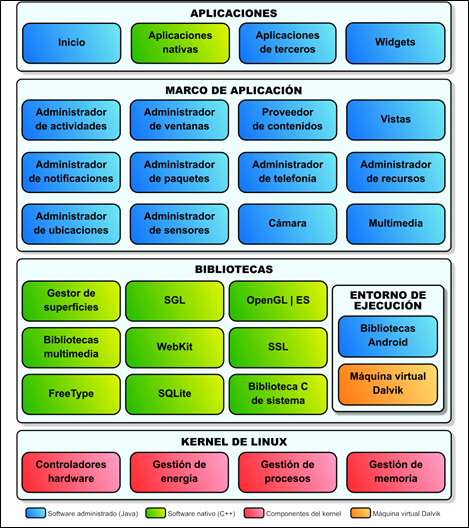
\includegraphics[scale=0.55]{C:/Users/usuario/Tesisworkspace/Tesis_Standalone/tesis/images/Android-architecture}
\par\end{centering}

\caption{Diagrama de la arquitectura en capas empleada por Android\label{fig:Android-architecture}}
\end{figure}


Las capas interactúan entre sí respetando el estilo arquitectónico
tradicional, donde cada una de las capas utiliza los servicios ofrecidos
por las anteriores, y ofrece a su vez sus propios servicios a las
capas de niveles superiores. 

Las diferentes capas de la arquitectura son descritas a continuación:
\begin{itemize}
\item Kernel Linux: Android utiliza el núcleo de Linux como una capa de
abstracción de hardware para los dispositivos móviles. Esta capa contiene
los drivers necesarios para que cualquier componente de hardware pueda
ser utilizado mediante las llamadas correspondientes, sólo debe considerarse
al momento de incluir un nuevo componente de hardware que los fabricantes
hayan desarrollado los drivers correspondientes. Además del soporte
de drivers, la capa es responsable de proporcionar otros servicios
como la seguridad, el manejo de la memoria, la gestión de procesos,
la pila de protocolos. 
\item Entorno de ejecución de Android: como se ha adelantado previamente,
cada aplicación corre en su propio proceso Linux con su propia instancia
de la máquina virtual Dalvik, la cual interpreta un lenguaje ligeramente
diferente al tradiciones de \ac{JVM} bajo el formato .dex. A partir
de la versión 5.0 de Android, Dalvik es reemplazada por \ac{ART}
la cual logra reducir el tiempo de ejecución del código Java hasta
un 33\%. También se incluye en el entorno un módulo de librerías nativas
con la mayoría de librerías disponibles en lenguaje Java. Estas bibliotecas,
si bien resultan diferentes a las ofrecidas por \ac{Java SE} y \ac{Java ME},
proveen prácticamente la misma funcionalidad. 
\item Bibliotecas: Incluye un conjunto de librerías en lenguaje C o C++
usadas en varios componentes de Android proporcionando la mayor parte
de las capacidades más características de Android, algunas de ellas
fueron expuestas en la figura anterior. En el caso de las bibliotecas
SQLite se provee acceso a la utilización y administración de bases
de datos \ac{SQL}. Estas librerías están compiladas en código nativo
del procesador y muchas de ellas utilizan proyectos de código abierto. 
\item Marco o entorno de Aplicaciones: Proporciona una plataforma de desarrollo
libre para aplicaciones con gran riqueza e innovaciones de herramientas
como sensores, localización, servicios, barra de notificaciones, entre
otros. y además permite que los desarrolladores tengan acceso a las
mismas \ac{API} utilizadas por las aplicaciones base del sistema.
El foco principal del diseño de esta capa ha sido simplificar la reutilización
de componentes, las aplicaciones pueden publicar sus capacidades y
otras pueden hacer uso de ellas (sujetas a restricciones de seguridad),
un mecanismo que permite a los usuarios reemplazar fácilmente componentes. 
\item Aplicaciones: Este nivel contiene todas las aplicaciones de usuario,
tanto las incluidas por defecto en Android así como como aquellas
que el usuario vaya añadiendo posteriormente ya sean de terceros o
de su propio desarrollo. Todas estas aplicaciones utilizan los servicios,
las \ac{API} y bibliotecas de los niveles inferiores. Se brindará
una descripción más detallada en la sección siguiente
\end{itemize}

\subsection{Aplicaciones Android \label{sec:Aplicaciones-Android}}

Además de las características técnicas, es importante resaltar que
la popularidad de Android ha crecido muy rápidamente desde su lanzamiento.
Esto se debe a la versatilidad que Android otorga a éstos dispositivos
a través de las aplicaciones, que permiten adaptarlos según las necesidades
de los usuarios. Además, el hecho de que Android sea de código abierto
da lugar a la creación de diferentes versiones del sistema operativo
que permiten personalizar cada aspecto del mismo. Android también
permite que las aplicaciones se adapten a las características del
dispositivo (pantalla, sensores, etc.), aprovechando las capacidades
de cada dispositivo particular. 

Respecto a las herramientas de desarrollo, Android ofrece un paquete
que combina el \ac{IDE} Eclipse con un conjunto de herramientas que
simplifican el desarrollo, permitiendo incluso, crear dispositivos
virtuales que emulan cualquier configuración de hardware soportada. 

Por otra parte, en el contexto de los servicios Web, Android provee
soporte para conexiones \ac{HTTP} , y por tanto, permite la utilización
de servicios Web \ac{REST} a través de ella. 

Un aspecto único del diseño de las aplicaciones en Android es que
éstas pueden reutilizar componentes de otras aplicaciones instaladas
en el dispositivo. Por ejemplo, si una aplicación desea tomar una
fotografía, es probable que ya exista una aplicación que cumpla esa
funcionalidad, entonces, la nueva aplicación puede utilizar la existente
sin necesidad de desarrollar una actividad propia para utilizar la
cámara, esta invocación se realiza de modo tal que sea transparente
para el usuario final.

El sistema Android provee cinco tipos de componentes básicos para
el desarrollo de aplicaciones. El componente \emph{Activity }representa
una pantalla simple y es el único que provee interfaz de usuario.
A través de estas actividades se logra el acceso a la información
almacenada en los componentes \emph{Content Provider }que son los
encargados de administrar la información compartida por las aplicaciones;
las aplicaciones pueden almacenar sus datos en el sistema de archivos,
en una base SQLite, en la Web, o en cualquier otro lugar de acceso.
A través del ‘content provider’, otras aplicaciones pueden consultar,
o incluso modificar estos datos. 

Las actividades también pueden iniciar servicios que se ejecutan en
segundo plano para realizar operaciones que requieran gran cantidad
de tiempo, o interactúen con procesos remotos, por ejemplo la reproducción
de música en segundo plano o la descarga de datos mientras el usuario
interactúa con una aplicación diferente. 

Respecto a los anuncios o mensajes de difusión masiva, el componente
\emph{Broadcast Receiver} funciona como puerta de enlace a otros componentes,
respondiendo mayormente a los anuncios originados por el sistema,
por ejemplo, cuando la pantalla se apaga, la batería es baja, o al
capturar una fotografía. 

El último componente denominado \emph{Intent} representa acciones
a realizar, específicamente, tienen por finalidad iniciar actividades,
servicios o \emph{Broadcast Receivers} realizando el binding en tiempo
de ejecución entre los componentes de las aplicaciones (tanto entre
componentes de una misma aplicación como de diferentes). Cada Intent
cuenta con una estructura de datos donde se realiza una descripción
abstracta de una operación a realizar, luego, la entrega de estos
objetos se realiza de diferente manera de acuerdo el tipo de componente
que se desee activar. 


\section{Componentes de software\label{sec:Componentes-de-software}}

En el marco del desarrollo de software para diferentes plataformas
y para móviles más específicamente, nos encontramos con la posibilidad
de reutilizar código previamente desarrollado, testeado y deployado
que cumpla con una determinada funcionalidad ahorrando tiempo y esfuerzo
al desarrollador. Estas piezas de códigos ya implementadas y disponibles
se conocen bajo el nombre de componentes de software e incluyen en
su definición paquetes de software, servicios o recursos web, o módulos
que encapsulan a un conjunto de funciones o datos relacionados; sin
embargo, cualquiera sea la pieza que represente, frecuentemente los
componentes son vistos y tratados como objetos o colección de objetos. 

La reutilización es uno de los objetivos principales al momento de
diseñar un nuevo componente de software de gran calidad para ser usados
en diferentes programas. Por lo tanto la implementación y diseño de
un componente conlleva un gran esfuerzo e incluye procesos complejos
como la documentación, testing robusto a través de entradas comprensibles
y la posibilidad de retornar mensajes de error y códigos, y el diseño
enfocado a la utilización en formas imprevistas. Si bien los componentes
actúan sin modificar su código, el comportamiento de los códigos fuentes
del componente puede cambiar basado en la extensibilidad de la aplicación. 

Todos los procesos de sistemas son estructurados bajo componentes
separados de modo tal que todos los datos y funciones de un componente
mantengan una misma relación semántica, principio que se mantiene
en el contenido de las clases. Por esta razón, se le atribuye a los
componentes las características de ser modulares y cohesivos. 

La comunicación entre componentes se realiza a través de interfaces.
Cuando un componente ofrece servicios al resto del sistema, el mismo
proporciona una interfaz que especifica los servicios que otros componentes
pueden utilizar y la manera en que pueden hacerlo. La interfaz puede
verse como una firma del componente ya que el cliente no necesita
conocer el procesamiento interno del componente para utilizarlo, condición
que respeta el principio de encapsulamiento. 

Por otro lado, cuando un componente necesita de otro para su funcionamiento,
el mismo establece las interfaces requeridas donde especifica los
servicios que necesita. 

De acuerdo al modelo \ac{UML} y lo reflejado en la figura \ref{fig:UML-component},
las interfaces proporcionadas son representadas con símbolos de lollipop
en el borde del componente y las interfaces requeridas por medio de
sockets abiertos en el borde externo. 

\begin{figure}
\begin{centering}
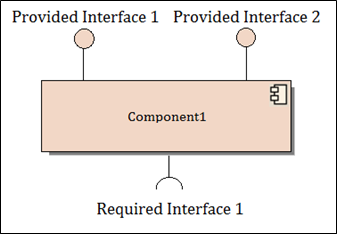
\includegraphics[scale=0.55]{C:/Users/usuario/Tesisworkspace/Tesis_Standalone/tesis/images/UML-component}
\par\end{centering}

\caption{Componente UML con interfaces proveídas y requeridas.\label{fig:UML-component}}
\end{figure}


Otra de las características fundamentales de los componentes es su
capacidad de ser sustituibles tanto en tiempo de diseño como en tiempo
de ejecución, pudiendo ser reemplazados por actualizaciones u otras
alternativas sin romper el sistema en el que los componentes funcionan.
El reemplazo es posible si el componente sucesor provee por lo menos
la misma funcionalidad que el componente a reemplazar y si requiere
a lo sumo las mismas funciones que el componente inicial. 


\section{Atributos de calidad \label{sec:Atributos-de-calidad}}

Al diseñar un sistema de software no sólo se espera cumplir con los
objetivos de negocio sino también alcanzar un determinado grado de
calidad de software capaz de satisfacer al grupo de usuarios y/o diseñadores,
muchos factores determinan las cualidades que deben proporcionarse
en la arquitectura de un sistema. Estas cualidades \cite{Ghahramani2004}
van más allá de la funcionalidad (capacidades), servicios y comportamientos
del sistema El diseño de la arquitectura de un sistema depende mayormente
de los atributos de calidad (también denominados propiedades no funcionales)
demandados por los stakeholders que de la funcionalidad en sí misma
que especifica el comportamiento que debería tener el producto, para
considerar un software de utilidad; largos tiempos de respuesta, caídas
del sistema, interfaces confusas, no son características deseables
en un sistema, por lo que toda decisión respecto al diseño de la arquitectura
debe conducir al cumplimiento de ciertos atributos de calidad al mismo
tiempo que cumple con la funcionalidad requerida. 


\subsection{Performance\label{subsec:Atributos-de-calidad-Performance}}

Se puede medir la calidad de un sistema a través de su desempeño evaluando
la efectividad del uso de los recursos disponibles en tiempo de ejecución.
Dependiendo el contexto, la eficiencia puede medirse a través de varios
parámetros, incluyendo tiempo de respuesta, ancho de banda y disponibilidad. 

El rendimiento de un sistema engloba, generalmente, el tiempo de los
eventos que se producen y que el sistema debe responder a ellos. Estos
eventos pueden ser muy variados tales como alarmas, mensajes, peticiones
a usuarios o simplemente tiempo de procesamiento, pero básicamente
se considera de todos ellos el tiempo que tarda el sistema para responder
ante el evento . La complejidad para el manejo de estos eventos radica
en su fuente, ya que pueden provenir desde una solicitud de usuario,
de otros sistemas o desde el interior del propio sistema. 

Sin importar el contexto de desarrollo del sistema, el patrón de los
eventos que llegan y el patrón de respuestas se pueden caracterizar,
y esta caracterización hace posible la construcción de escenarios
generales de rendimiento empleados en diferentes benchmarks, por ejemplo
el tiempo de respuesta puede significar el tiempo máximo y mínimo
de procesamiento para cierto elemento del sistema o la cantidad máxima
de eventos que un determinado servicio puede atender por unidad de
tiempo. 

La respuesta del sistema a un estímulo puede ser caracterizado por
la latencia (el tiempo entre la llegada del estímulo y la respuesta
del sistema a la misma), los plazos de procesamiento, la fluctuación
de la respuesta (la variación de latencia), el número de eventos no
procesados debido a que el sistema era demasiado ocupado para responder,
y los datos que se perdió debido a que el sistema era demasiado ocupado. 


\subsection{Precisión\label{subsec:Atributos-de-calidad-Precisi=0000F3n}}

Cabe destacar que no existe una definición estándar sobre el significado
de precisión en un sistema, ya que se trata de una medida que evalúa
qué tan exacta es la respuesta de un componente, y cada componente
está fuertemente ligado al dominio en el que se presenta, por ejemplo,
en un problema de detección de rostros, la precisión puede significar
la cantidad de rostros correctamente detectados sobre los rostros
totales presentes, y en un problema de clasificación puede significar
la correctitud en la predicción de la clase para un cierto atributo.

En términos generales, se toma la precisión como el grado de cercanía
(o dispersión) de las mediciones respecto al verdadero valor, es el
grado en que si las mediciones se repitieran bajo las mismas condiciones
los resultados serían los mismos. A menudo, la medida de precisión
es confundida con el término exactitud que indica la distancia del
valor medido respecto al valor verdadero. Por ejemplo, si un experimento
contiene un error sistemático, el aumento del tamaño de la muestra
en general aumenta la precisión, pero no mejora la exactitud. El resultado
sería una cadena consistente (aunque incorrecto) de los resultados
del experimento defectuoso. La eliminación del error sistemático mejora
la exactitud, pero no cambia la precisión. 


\section{Aprendizaje de máquina \label{sec:Aprendizaje-de-maquina}}

El aprendizaje a partir de datos es la base para comprender el proceso
de aprendizaje de máquina ya que los datos son la única herramienta
de la que se dispone y conoce a ciencia cierta sobre las características
de un dominio cualquiera. La representación de los datos reales puede
alcanzar el tamaño de terabytes por lo que dificulta hacer una analogía
respecto al aprendizaje humano basado en la experiencia. 

El hombre basa su conocimiento en tres partes: \emph{i}) recuerdo,
el hombre reconoce cuando ha sido la última vez que se estuvo en una
determinada situación (dataset), \emph{ii}) adaptación, reconoce la
última vez que se probó una acción (salida producida) y \emph{iii})
generalización, si ha funcionado o no (si fue correcta o no). 

El término generalización refiere a la similitud entre diferentes
situaciones de manera tal que las opciones que han sido aplicadas
en casos previos pueden ser usadas en nuevos casos. Estas fueron las
bases del primer Aprendizaje Artificial y es conocido como procesamiento
de símbolos ya que las computadoras manipulan símbolos que reflejan
el ambiente. En contraste, los métodos de aprendizaje de máquinas
son llamados sub-simbólicos ya que no se utilizan símbolos. 

El aprendizaje de máquina, entonces, es un proceso para que las computadoras
modifiquen o adapten sus acciones (predictivas o de control de robot)
para que sus resultados sean más precisos, precisión que refleja la
proximidad respecto a las acciones correctas. El aprendizaje de máquina
reúne ideas de neurociencia y biología, estadística, matemática y
física, para generar técnicas y hacer que la computadora aprenda.
Otro concepto importante en este ámbito es la minería de datos, el
proceso de extraer información útil de un conjunto de datos masivos
llamado comúnmente dataset por medio de algoritmos de alto grado de
eficiencia y enfatizados nuevamente en la ciencia computacional. 

Quizás, el punto de inflexión en este campo de estudio es la complejidad
computacional de la aplicación de técnicas de aprendizaje de máquina
sobre un gran volumen de datos, de manera que los algoritmos de complejidad
polinomial muy grande pueden resultar un problema. Generalmente la
complejidad se divide en dos partes: la complejidad del entrenamiento
y la complejidad de aplicar el algoritmo entrenado. El proceso de
entrenamiento usualmente, se realiza escasas veces, incluso tan sólo
una, y el tiempo que requiere no resulta tan crítico, por lo que se
enfatiza sobre la segunda parte donde se pretende que la decisión
sea lo más rápida posible con un bajo costo computacional. 

Si se define en forma imprecisa el concepto de aprendizaje como la
mejora de tareas a través de la práctica surgen algunos cuestionamientos
asociados, de qué forma la computadora puede saber si está aprendiendo
mejor o de qué forma podría mejorar ese aprendizaje. De aquí, toman
lugar diferentes tipos de aprendizaje de máquina, por ejemplo se le
puede indicar a un algoritmo la respuesta correcta para un problema,
así, la próxima vez que se aplique su desempeño será mejor. También,
podría indicarse un conjunto de respuestas correctas para que la máquina
\emph{adivine} la forma de obtener estas respuestas para otros problemas
(generalización). Alternativamente, se puede indicar si la respuesta
obtenida es correcta o no sin señalar la respuesta real ya que la
máquina debería ser capaz de encontrarla; una variante podría ser
asignarle un puntaje a la respuesta obtenida por el algoritmo acordando
cuán correcta resulta ser y no sólo indicarlo mediante los valores
verdadero o falso. 

Estas diferentes respuestas proveen una forma fácil de clasificar
los diferentes métodos de aprendizaje, los cuales serán detallados
en las secciones siguientes en base a la naturaleza de la entrada
y la naturaleza de la salida; sin embargo todos los métodos comparten
el mismo objetivo de generalización: el algoritmo debe producir salidas
sensibles para datos de entrada que no fueron encontrados durante
el aprendizaje teniendo en cuenta también que el algoritmo puede lidiar
con ruido en los datos, una pequeña imprecisión en los valores que
es inherente a la medición de cualquier proceso real. 


\subsection{Clasificación por la naturaleza de la entrada}

El modo de aprendizaje que un algoritmo particular puede realizar
queda determinado por la naturaleza de los datos de entrada, es decir,
puede variar en base a la información contenida en los datos de entrenamiento
(\emph{training set}). 

El aprendizaje supervisado utiliza un conjunto de datos basado en
dos pares de objetos: los datos de entrada o conjunto de ejemplos
del dominio y las respuestas correctas (\emph{targets}) para una determinada
característica; a través de las respuestas correctas provistas y basado
en el conjunto de datos el algoritmo de aprendizaje generaliza el
comportamiento para responder a todas las posibles entradas. Este
modo de aprendizaje, entonces, es un proceso que se realiza mediante
un entrenamiento controlado por un agente externo que determina la
respuesta que debería generar el algoritmo a partir de una entrada
determinada. 

Contrariamente, el aprendizaje por refuerzo se basa en la idea de
no disponer de ejemplos completos del comportamiento deseado por el
algoritmo, es decir, no indicar durante el entrenamiento exactamente
la salida que se desea proporcione el clasificador ante una determinada
entrada, sólo se le indica si la salida obtenida se ajusta a la deseada
y en función a ello se re configuran los pasos. 

Por último, en el aprendizaje \cite{Ghahramani2004} no supervisado,
la máquina simplemente recibe los datos de entrada sin etiquetas o
respuestas correctas como en el método supervisado ni valores de recompensa
desde el ambiente, dando lugar a una percepción misteriosa sobre la
forma que se espera que el método aprenda sin recibir ningún tipo
de devolución. Sin embargo, es posible desarrollar un framework formal
para llevar a cabo aprendizaje no supervisado basado en la noción
de que el objetivo es construir una representación de la entrada que
puede ser usada para tomar decisiones, predecir futuras entradas,
comunicar eficientemente entradas para otras máquinas, entre otras
posibilidades. El aprendizaje no supervisado puede entenderse como
la búsqueda de patrones en los datos independientemente del ruido
presente en los mismos. 

Nótese que los valores de entrada y etiqueta describen vectores ya
que cada ejemplo (\emph{instance}) del conjunto de entrenamiento posee
varias características (\emph{features}); si se tuvieran todos los
posibles ejemplos de un problema, no habría necesidad alguna de aprendizaje.


\subsection{Clasificación por la naturaleza de la salida}

La teoría de aprendizaje de maquinas abarca varios factores considerando
las características de lo que se busca en los diferentes métodos.
Así, existen cinco tipos de métodos, para la búsqueda de diferentes
objetivos:
\begin{description}
\item [{Clasificación}] Consiste en asignar a cada ejemplo una etiqueta
o clase a la que pertenece basado en el entrenamiento de ejemplares
de cada clase. Los datos de entrenamiento son instancias que pertenecen
a una única clase y el conjunto de clases cubre todas las salidas
posibles, por eso se considera al proceso de clasificación como un
proceso discreto. El algoritmo de clasificación tiene como objetivo
encontrar umbrales de decisión que sirvan para identificar las diferentes
clases.
\item [{Clustering}] El proceso de clustering es la tarea de agrupar un
conjunto de objetos de modo tal que los objetos pertenecientes a un
mismo grupo (\emph{cluster}) comparten algún tipo de similitud entre
ellos, de igual sentido que se diferencian con los objetos de otro
grupo. A diferencia del proceso de clasificación, los grupos o clases
no son conocidos fehacientemente antes del entrenamiento, un claro
método de aprendizaje no supervisado. 
\item [{Estimación~de~densidad}] La función de densidad de probabilidad
\cite{Silverman1986} es un concepto fundamental de la estadística
y caracteriza el comportamiento probable de una población en tanto
especifica la posibilidad relativa de que una variable aleatoria continua
X tome un valor cercano a x.
\item [{Reducción~de~dimesionalidad}] Se basa en simplificar los datos
de entrada mapeándolos en un espacio dimensional más simple.
\item [{Regresión}] El proceso de regresión predice valores numéricos de
atributos a partir de funciones matemáticas polinomiales que describan
o se ajusten lo más posible a todos los puntos del dominio, es decir,
todos los valores del conjunto de entrenamiento correspondientes al
atributo que se quiere predecir. Generalmente, se considera un problema
de aproximación de función o interpolación al encontrar un valor numérico
entre los valores conocidos. Por lo tanto, el eje primordial del proceso
de regresión es encontrar la función que mejor represente al conjunto
de puntos, ya que funciones con distintos grados de polinomios causan
diferentes efectos. La figura \ref{fig:regression-problems} refleja
la situación expresada anteriormente, donde se muestra el conjunto
de valores del dominio y tres curvas alternativas de representación.
El gráfico inferior izquierdo combina, además, una función cúbica
y línea recta. 
\end{description}
\begin{figure}
\begin{centering}
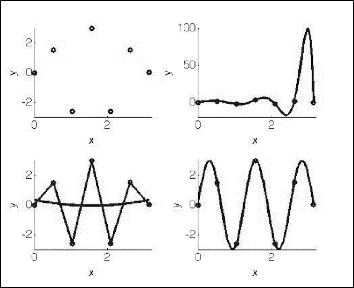
\includegraphics[scale=0.55]{C:/Users/usuario/Tesisworkspace/Tesis_Standalone/tesis/images/regression-problems}
\par\end{centering}

\caption{Comparación de distintas funciones polinomiales de regresión. \label{fig:regression-problems}}
\end{figure}


La forma más correcta de saber cuál solución presentada es la mejor,
se evalúa el grado de generalización que permite cada una; se toma
algún punto incluido entre los puntos ya representados y se utiliza
la curva para predecir el valor, luego se compara entre los valores
para saber cual resultó más próximo. En este caso, el gráfico inferior
derecho. 

~

Cabe destacar que en el presente trabajo, se analizan técnicas de
regresión, ya sea aquellas que intrínsecamente representan funciones
polinomiales como aquellas que se adaptaron desde los métodos de clustering
para la obtención de valores densos.


\subsection{Funciones contempladas\label{subsec:Funciones-contempladas}}

El foco principal del trabajo desarrollado ha sido guiado por la búsqueda
de predicción de valores numéricos sobre componentes de ejecución,
como el uso de CPU, consumo de red, precisión y desempeño de las respuestas,
entre otros. Estos indicadores son valores continuos, motivo por el
cual se utilizaron modelos de regresión, los mismos se describirán
en las subsecciones siguientes. 


\subsubsection{Regresión Lineal\label{sub:Regresi=0000F3n-Lineal}}

La regresión es la predicción de un valor desconocido a través del
cálculo de una función matemática a partir de los valores conocidos.
Si se considera esta función como una línea recta, la salida será
la suma de cada valor conocido multiplicado por una constante la cual
define la línea recta (plano en 3D o hiperplano en dimensiones mayores)
que circundan los puntos como puede observarse en la figura \ref{fig:regression-lineal}. 

\begin{figure}
\begin{centering}
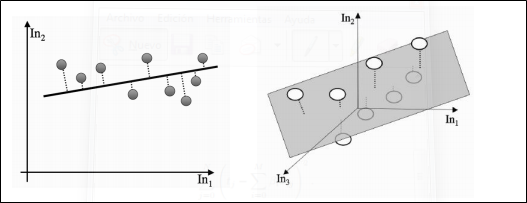
\includegraphics[scale=0.55]{C:/Users/usuario/Tesisworkspace/Tesis_Standalone/tesis/images/regression-lineal}
\par\end{centering}

\caption{Algoritmo Linear regression en dos y tres dimensiones.. \label{fig:regression-lineal}}
\end{figure}


Para encontrar la recta que mejor se adapte a los datos se intenta
minimizar la distancia entre cada punto y dicha línea, esta distancia
se mide a través de una línea auxiliar que atraviese el punto y tope
con la función, por ejemplo mediante el Teorema de Pitágoras. Luego,
se intentará minimizar la función de error que mide la suma de cada
distancia, si se ignora las raíces y sólo se minimiza la suma de los
cuadrados de los errores, se obtiene la minimización más común llamada
optimización de mínimos cuadrados. 

La minimización de esta función da lugar a la implementación de diversas
alternativas de la función lineal. En el presente trabajo se desarrollan
dos variantes, la función denominada \emph{ridge-regression }y la
función \emph{gradiente estocástico descendiente}. La primera aplica
una penalización (\emph{ridge}) a cada constante. La segunda, aplica
un diferencial sobre la función obteniendo el gradiente el cual por
definición, es la dirección en la que incrementa o disminuye en mayor
medida. Ya que el propósito del aprendizaje es minimizar el error
de predicción, se debe seguir la función en dirección del gradiente
negativo en la cual la función disminuye. 


\subsubsection{Red neuronal}

Se presenta un modelo matemático sobre el comportamiento de una neurona,
el modelo neuronal McCulloch - Pitts denominado así debido a sus creadores
Warren McCulloch y Walter Pitts, ambos produjeron un ejemplo perfecto
al modelar una célula nerviosa como \emph{i}) un conjunto de entradas
valoradas (w\textsubscript{i}) que corresponde a las sinapsis, \emph{ii})
un sumador que une las señales entrantes (equivalente a la membrana
de la célula que recolecta la carga eléctrica) y \emph{iii}) una función
de activación (inicialmente una función umbral) que decide sobre la
activación de la célula en base a las entradas actuales. 

\begin{figure}
\begin{centering}
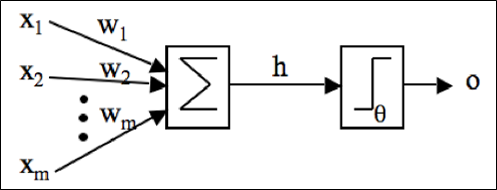
\includegraphics[scale=0.55]{C:/Users/usuario/Tesisworkspace/Tesis_Standalone/tesis/images/McCulloch-Pitts}
\par\end{centering}

\caption{Modelo matemático neuronal McCulloch - Pitts. \label{fig:McCulloch-Pitts}}
\end{figure}


Como puede observarse en la figura \ref{fig:McCulloch-Pitts}, el
modelo McCulloch - Pitts es un dispositivo límite binario, las entradas
son multiplicadas por los pesos o fuerzas sinápticas y luego se suman
sus valores, si la suma es mayor a un determinado umbral (produce
salida 1) la célula se activa, de lo contrario (produce salida 0)
se mantiene desactivada. Teniendo en cuenta que una red neuronal puede
llevar a cabo cualquier cálculo que realiza una computadora normal,
los pesos o valores de la fuerza sináptica deben ser elegidos correctamente,
considerando en consecuencia, un método capaz de configurar dichos
pesos. Observando la neurona McCulloch y Pitts, se puede notar fácilmente
que las entradas son independientes al cerebro, por lo que sólo cambia
el valor de los pesos y el umbral. Considerando que el aprendizaje
sucede entre las neuronas y éstas están conectadas mutuamente, se
debe tener en cuenta la manera en que en cambian los pesos y los umbrales
de las neuronas para que la red pueda obtener la respuesta correcta
más frecuentemente.

Teniendo en cuenta que una red neuronal puede llevar a cabo cualquier
cálculo que realiza una computadora normal, los pesos o valores de
la fuerza sináptica deben ser elegidos correctamente, considerando
en consecuencia, un método capaz de configurar dichos pesos.

Observando la neurona McCulloch y Pitts, se puede notar fácilmente
que las entradas son independientes al cerebro, por lo que sólo cambia
el valor de los pesos y el umbral. Considerando que el aprendizaje
sucede entre las neuronas y éstas están conectadas mutuamente, se
debe tener en cuenta la manera en que en cambian los pesos y los umbrales
de las neuronas para que la red pueda obtener la respuesta correcta
más frecuentemente. 


\subsubsection*{Red Neuronal Perceptron }

El perceptrón es una colección de neuronas McCulloch y Pitts con un
conjunto de entradas y pesos que unen las neuronas con dichas entradas. 

\begin{figure}
\begin{centering}
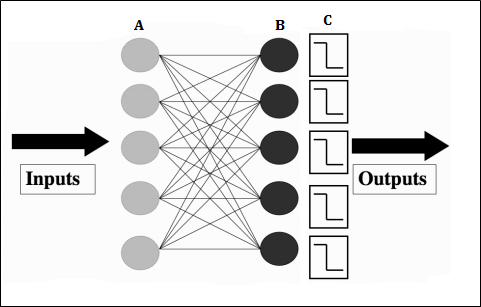
\includegraphics[scale=0.55]{C:/Users/usuario/Tesisworkspace/Tesis_Standalone/tesis/images/perceptron-neural-network}
\par\end{centering}

\caption{Red neuronal perceptron\label{fig:perceptron-neural-network}}
\end{figure}


Como puede observarse en el gráfico de la figura \ref{fig:perceptron-neural-network},
las neuronas del Perceptrón son completamente independientes entre
sí, el estado de una neurona no infiere sobre las demás, sólo comparten
las entradas. Un punto a destacar es que el número de entradas y de
neuronas no necesariamente debe corresponderse, en general hay \emph{m}
entradas y \emph{n} neuronas. 

El mayor inconveniente es conocer con certeza los valores que deben
tener los pesos para que las salidas sean las correctas, esta es la
finalidad de la red neuronal, aprender si determinada neurona debe
o no activarse de forma correcta. 

Un proceso de análisis sobre los pesos podría arrojar que los pesos
toman valores muy grandes en la activación de una neurona (cuando
no debería hacerlo) o en caso contrario, valores muy pequeños, por
lo que se podría computar una función de error como la diferencia
entre la salida que produjo la neurona y la salida de la red. En el
caso particular de entradas en cero, se modifica el valor de umbral
añadiendo a la red Perceptron un parámetro extra denominado bias,
los pesos de esta entrada son usualmente asignados al índice cero. 


\subsubsection*{Red neuronal Perceptrón multicapa }

La esencia del aprendizaje de la red neuronal perceptrón está centrada
en los valores de pesos, una buena práctica entonces, sería la incorporación
de nuevos pesos. Como alternativa para ello podrían agregarse conecciones
hacia atrás para conectar las neuronas de salida con las entradas
nuevamente, o podrían agregarse nuevas neuronas creando redes mucho
más complejas, como el caso reflejado en la figura \ref{fig:perceptron-neural-network-multilayer}
donde se representa un modelo perceptrón de tres capas con cinco entradas,
tres salidas y tres neuronas en la capa oculta.

\begin{figure}
\begin{centering}
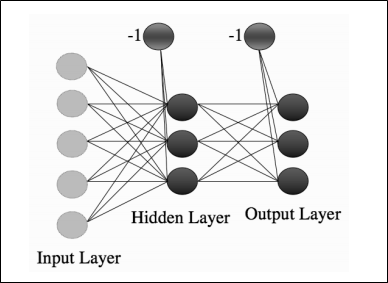
\includegraphics[scale=0.55]{C:/Users/usuario/Tesisworkspace/Tesis_Standalone/tesis/images/Perceptron-multilayer}
\par\end{centering}

\caption{Red perceptrón multicapa\label{fig:perceptron-neural-network-multilayer}}
\end{figure}


La nueva red, ahora, debe ser entrenada para que los pesos nuevos
se adapten y generen las respuestas correctas (\emph{targets}). Estas
respuestas son conocidas y se puede computar la diferencia entre estas
y las salidas pero se desconoce si el peso incorrecto pertenece a
la primera capa o a la segunda y cuáles activaciones de las neuronas
de la capa intermedia son correctas, razón por la cual esta capa se
denomina capa oculta ya que es imposible examinar y corregir sus valores
de forma inmediata. 

El entrenamiento de \ac{MLP} consiste en dos partes, primero se obtienen
las salidas con las entradas brindadas y los pesos actuales (\emph{forwards}),
y luego se actualizan los pesos considerando el error como la diferencia
entre el valor obtenido y el real (propagación hacia atrás del error
- \emph{backwards}). 

Por lo tanto, con la función de error y de activación, puede calcularse
el diferencial para modificar los pesos en dirección del gradiente
negativo, mejorando así la función de error. El objetivo es obtener
los gradientes de esos errores y usarlos para decidir cuánto deben
actualizarse dichos pesos en la red sobre la capa de salida y, luego
de actualizarla, se opera hacia atrás (\emph{backwards}) a través
de la red hasta llegar a la entrada nuevamente. Sólo existen dos problemas,
para las neuronas de salida se desconocen las entradas que le corresponden
y para las neuronas escondidas, se desconocen las salidas esperadas
(\emph{targets}) y en caso de existir más capas incluso podrían no
conocerse las entradas. Para solucionar estas cuestiones se aplica
la regla de la cadena la cual afirma que para conocer la forma en
que varía el error en base a la variación de los pesos, se debe analizar
la variación del error en función de las entradas de los pesos y multiplicarlo
por el valor de la variación de los pesos según la variación de entradas. 

Esta forma de resolución es muy útil ya que permite conocer todas
las derivadas que se necesitan. Puede escribirse la función de activación
de los nodos de salida en términos de los nodos ocultos y de los pesos
de salida para luego enviarlo hacia las capas ocultas de la red (hacia
atrás) para decidir cuáles eran los salidas esperadas para esas neuronas.


\subsubsection{K-means clusterer}

El algoritmo K - means aplica clustering sobre los datos de entrenamiento
y recibe un parámetro \emph{K} para dividir estos datos en \emph{K}
categorías. El algoritmo intenta localizar k centros en el espacio
de entrada de modo tal que estos centros estén, como su nombre lo
indica, en el centro de una categoría (\emph{cluster}). La dificultad
se presenta ya que al desconocer la categorización de estos grupos,
resulta aún más difícil determinar la localización de cada centro. 

Los algoritmos de aprendizaje generalmente se basan en minimizar alguna
clase de error, en consecuencia la primera acción que se realiza es
definir un criterio que lo describa teniendo en cuenta: \emph{i})
una medida de la distancia entre puntos, definir una medida para cuantificar
estas distancias, por lo general se usa la distancia euclídea y \emph{ii})
determinar el punto central de un conjunto de puntos (\emph{mean average})
considerando el espacio euclídeo ya que en espacios curvos es otra
la interpretación. Teniendo en cuenta estos conceptos, el algoritmo
K - means calcula el punto medio (centro) de cada cluster (µ\textsubscript{c}(i)).
lo que resulta equivalente a minimizar la distancia euclídea de cada
punto del cluster al centro del mismo. 

El objetivo de determinar estos centros, en principio, a causa de
incertidumbre total se posicionan los centros de forma aleatoria en
el espacio de entrada. Una vez distinguidos los clusters, se determinar
los puntos que pertenecen al mismo a través del cálculo de la distancia
entre el punto y todos los centros localizados, asignándose entonces,
al cluster cuyo centro sea el más cercano. Finalmente, para cada centro
se actualiza su ubicación utilizando la media antes definida. Estos
pasos se realizan de forma incremental hasta que los centros dejar
de modificar su ubicación. 

Ya que este algoritmo sin duda es un método de clasificación y no
de regresión, se considera importante resaltar la adaptación del mismo
para utilizarlo con este fin. Así, una vez realizada la clasificación
del punto que se quiere predecir, se realizará la predicción calculando
el promedio de los valores del atributo a predecir de los otros puntos
que están en el cluster. 


\subsubsection{Maquina de vector de soporte}

Al tratar con problemas de clasificación existen varios clasificadores
lineales que ofrecen respuestas correctas pero diferentes, como se
expone en la figura \ref{fig:lineals-classifiers}. Si bien las soluciones
laterales son acertadas, las líneas divisorias son muy próximas a
algunos puntos del conjunto de datos de entrenamiento dando paso a
una posible imprecisión futura en la predicción, situación que no
se observa en el ejemplo central de la figura. 

\begin{figure}
\begin{centering}
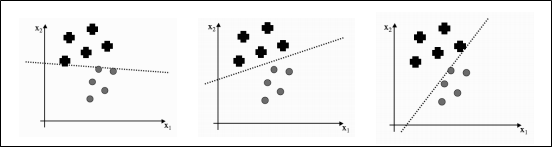
\includegraphics[scale=0.55]{C:/Users/usuario/Tesisworkspace/Tesis_Standalone/tesis/images/lineals-classifiers}
\par\end{centering}

\caption{Comparación de tres clasificadores lineales distintos.\label{fig:lineals-classifiers}}
\end{figure}


Analíticamente, se toma la distancia existente entre la línea y el
primer punto interceptado (en dirección perpendicular), si se ubica
una ‘zona desierta’ alrededor de la línea, ningún punto ubicado en
dicha zona puede ser clasificado ya que se encuentra demasiado cerca
de la línea. Esta región conforma un cilindro simétrico alrededor
de la función en 3D y un hiper - cilindro en dimensiones mayores.
El radio máximo que puede tener esta región es llamado margen, señalado
como M y los puntos de cada clase más cercanos a la línea de clasificación
se denominan vectores de soporte. Si se considera el mejor clasificador
como aquel que atraviesa la zona desierta, se debe tener en cuenta
que el margen debe ser lo más grande posible y que si los vectores
de soporte son los puntos más importantes de los datos, luego del
entrenamiento pueden descartarse los puntos que no pertenecen al vector
y utilizarlos para clasificar, lo cual conlleva una gran eficiencia
en el almacenamiento de datos. El algoritmo puede encontrar varios
hiperplanos de separación posibles y detectar aquel que sea más óptimo.
En la figura \ref{fig:SVM-metology} se reflejan estas dos situaciones
y se expone, en el gráfico derecho las notaciones matemáticas formales
del algoritmo. 

\begin{figure}
\begin{centering}
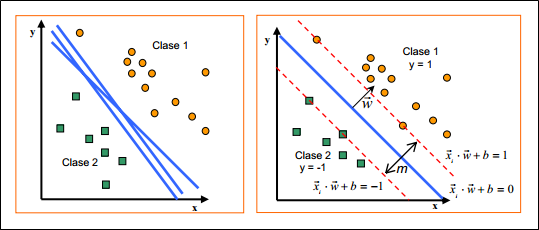
\includegraphics[scale=0.55]{C:/Users/usuario/Tesisworkspace/Tesis_Standalone/tesis/images/SVM-metology}
\par\end{centering}

\caption{Metodología de operación del algoritmo SVM\label{fig:SVM-metology}}
\end{figure}


A través de la función \emph{g(x) = w\textsuperscript{t}x + b} se
definen los dos hiperplanos (clasificador). Para obtener el punto
más cercano desde la línea de clasificación considerando la clase
2 (ver figura \ref{fig:SVM-metology}) se recorre en dirección perpendicular
partiendo del límite de la clase 1 hasta llegar al límite de la clase
2, el primer punto interceptado se denomina x. Para obtener un clasificador
de buena calidad, se pueden definir un conjunto de restricciones que
indiquen la manera en que el clasificador podría obtener la respuesta
correcta. Por ejemplo, si en lugar de tomar las dos clases como \emph{g(x)
= 1} y \emph{g(x) = 0}, se podrían igualar a los valores 1 y -1 y
así obtener una respuesta correcta diferente. Estos tipos de problemas
pueden ser resueltos de forma directa y eficiente (por ejemplo, en
tiempo polinomial), gracias a que existen algoritmos de programación
cuadrática que brindan soluciones efectivas.

Todas las consideraciones expuestas hasta el momento se realizaron
tras la asunción de que los datos podían ser divididos con funciones
lineales, pero no siempre es posible, en este caso la solución es
introducir variables. Estas variables indican que, al comparar clasificadores,
si uno clasifica un punto en un lado incorrecto y el otro lo ubica
mucho más lejos (también en un lado incorrecto) el primero es mejor
que el segundo, el error no fue tan extremo como en el segundo y esta
información debe ser incluida en los criterios de minimización modificando
las restricciones, incluyendo un parámetro \emph{C}. \emph{C} es el
parámetro que indica el trade off que existe entre ambos parámetros:
cuanto más pequeño sea el valor de C más importancia toma el margen
sobre algunos errores, cuanto más grande se vuelve C ocurre lo contrario.
Esto transforma el problema en un clasificador de margen suave ya
que se permiten algunos errores. La forma de evitarlos es modificando
las características para que los datos sean linealmente separables,
los datos no pueden inventarse de modo que las características deben
ser derivadas a partir de las existentes. Para ello se describe una
nueva función llamada kernel denominada \emph{φ(x)} que se aplica
sobre las diferentes variables de entrada, su función principal es
transformar los datos para obtener un espacio de dimensión mayor.
Como función kernel puede utilizarse cualquier función simétrica que
está definida positivamente (positividad de la integral de funciones
arbitrarias). Incluso, la conjunción de dos funciones kernel significa
una nueva función kernel. Elegir la función kernel más conveniente
es un problema complejo. A pesar que existen algunas teorías, el proceso
más común es la experimentación con distintos valores para determinar
la función más adecuada utilizando el conjunto de validación. El algoritmo
que aplica vectores de soporte se rige bajo todos los conceptos expresados
a lo largo del apartado para realizar clasificación, pero también
aplica para realizar regresión sobre los datos, variante que fue utilizada
en el presente trabajo. La figura \ref{fig:SVM-regression} muestra
un ejemplo de la aplicación del algoritmo SVM para regresión. 

\begin{figure}
\begin{centering}
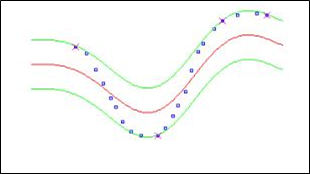
\includegraphics[scale=0.55]{C:/Users/usuario/Tesisworkspace/Tesis_Standalone/tesis/images/SVM-regression}
\par\end{centering}

\caption{Algoritmo SVM para regresión con función kernel de base radial.\label{fig:SVM-regression}}
\end{figure}



\subsection{Evaluación de modelos}

La evaluación del rendimiento de un modelo es una de las fases principales
en el proceso de ciencia de datos. Indica el nivel de acierto de las
predicciones del conjunto de datos mediante un modelo entrenado. Existen
dos formas para evaluar: evaluar el modelo y validar el modelo de
forma cruzada. Estos métodos permiten conocer el rendimiento del modelo
como un número de métricas que se usan habitualmente en estadísticas
y aprendizaje automático. La evaluación y la validación cruzada son
métodos estándares para medir el rendimiento de un modelo. Ambos generan
métricas de evaluación que sirven para inspeccionar y comparar con
las de otros modelos. 

La evaluación se basa en los valores predictivos junto con las etiquetas
o valores verdaderos. De forma alternativa, es posible usar la validación
cruzada para realizar automáticamente varias operaciones de entrenamiento,
puntuación y evaluación (10 subconjuntos) en distintos subconjuntos
de los datos de entrada. Los datos de entrada se dividen en 10 partes,
donde una se reserva para las pruebas y las otras 9 para el entrenamiento.
Este proceso se repite 10 veces y se calcula el promedio de las métricas
de evaluación. Esto ayuda a determinar el nivel al que un modelo se
podría generalizar para nuevos conjuntos de datos. 

El presente trabajo implementa las siguientes métricas de evaluación
para los modelos de regresión: 
\begin{itemize}
\item CC (Coeficiente de correlación de Pearson)
\item MAE (Mean Absolute Error) 
\end{itemize}
\[ \frac{1}{N}\sum_{i=1}^{N}{f_i-y_i}
\]
\begin{itemize}
\item RMSE (Root Mean Absolute Error)
\end{itemize}
\[ \sqrt{\frac{1}{N}\sum_{i=1}^{N}{f_i-y_i}^2}
\]
\begin{itemize}
\item RAE (Relative Absolute Error)
\end{itemize}
\[ \frac{\sum_{i=1}^{N}{|f_i-y_i}|}{\sum_{i=1}^{N}{|\overline{f_i}-y_i}|}
\]
\begin{itemize}
\item RRSE (Root Relative Squared Error)
\end{itemize}
\[ \sqrt{\frac{\sum_{i=1}^{N}{(f_i-y_i)^2}}{\sum_{i=1}^{N}{(\overline{f_i}-y_i)^2}}}
\]
\begin{itemize}
\item COMB
\end{itemize}
\[ (1-CC)+RRSE+RAE
\]
\begin{itemize}
\item SIMPLE ERROR
\end{itemize}
\[ \sum_{i=1}^{N}{(f_i-y_i)^2}
\]

El término \emph{error }representa la diferencia entre el valor predicho
y el valor verdadero. Normalmente, se calcula el valor absoluto o
el cuadrado de esta diferencia para capturar la magnitud total de
errores en todas las instancias, dado que la diferencia entre el valor
verdadero y el predicho puede ser negativa en algunos casos. Las métricas
de error miden el rendimiento de predicción de un modelo de regresión
en cuanto a la desviación media de sus predicciones a partir de los
valores reales. Los valores de error más bajos implican que el modelo
es más preciso a la hora de realizar predicciones. Una métrica de
error general de 0 significa que el modelo se ajusta a los datos perfectamente.


\subsection{Ajuste del modelo: Overfitting y Underfitting\label{sub:Ajuste-del-modelo:}}

Cuando un clasificador es entrenado se genera un modelo de predicción
cuya calidad es incierta hasta su aplicación. En algunas ocasiones,
la calidad del modelo es pobre generando respuestas imprecisas, de
modo tal que se le deben aplicar acciones correctivas comprendiendo
cómo se comporta y ajusta el modelo. 

Los modelos pueden presentar dos efectos indeseables . El efecto de
\emph{overfitting }describe una función que se ajusta estrechamente
a los datos de entrenamiento, el modelo aprendió los detalles y el
ruido en los datos impactando negativamente en el desempeño del modelo,
ha sido incapaz de generalizar. Este efecto es causado porque el ruido
o las fluctuaciones aleatorias en los datos de entrada fueron usados
para el aprendizaje. Los problemas de overfitting son más probables
en modelos no parametrizados y no lineales, los cuales tienen mayor
flexibilidad al aprender funciones. Por lo tanto, muchos algoritmos
de aprendizaje de máquina no parametrizados incluyen parámetros o
técnicas para limitar y restringir los detalles que el modelo aprende.
Por ejemplo, los árboles de decisión son algoritmos de aprendizaje
no parametrizados muy flexibles y pueden estar sujetos al efecto de
overfitting, en cuyo caso se procede a podar el árbol una vez que
el aprendizaje sea suficiente, eliminando así algunos detalles innecesarios.
Para solucionar este efecto se debe modificar el grado del polinomio
de la función utilizada por el modelo. 

Por otro lado, los modelos pueden presentar efectos de \emph{underfitting},
funciones que no interpretan o definen los datos de entrenamiento,
por lo que son incapaces de generalizar correctamente nuevos datos,
este efecto es causado porque la función o modelo elegido no es el
indicado para representar el comportamiento de los datos, el efecto
underfitting se caracteriza por sobre generalizar los datos. La incorporación
de nuevos datos al conjunto de entrenamiento podría solucionar o apaciguar
este efecto. 

El modelo deseado, sin dudas, sería aquel que se encuentre en un punto
de equilibrio entre modelos con underfitting y overfitting, aunque
esta eficiencia es muy difícil de alcanzar en la práctica. La figura
\ref{fig:under-overfitting} refleja el contraste entre los tres posibles
estados de un modelo. 

\begin{figure}
\begin{centering}
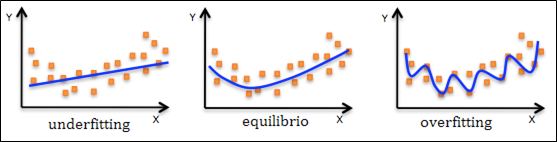
\includegraphics[scale=0.55]{C:/Users/usuario/Tesisworkspace/Tesis_Standalone/tesis/images/under-overfitting}
\par\end{centering}

\caption{Contraste entre distintos efectos del modelo sobre los datos de entrenamiento.\label{fig:under-overfitting}}
\end{figure}


El análisis de ambos efectos, se realiza gráficamente describiendo
la performance del algoritmo y la forma en que va aprendiendo a través
del tiempo. Al graficar la habilidad basada en los datos de entrenamiento
y en los datos de validación (testing), puede notarse que el error
basado en en el último gráfico de la figura \ref{fig:under-overfitting}
comienza a disminuir por efectos de overfitting ya que comienza a
aprender datos irrelevantes y ruidos del conjunto. En cuanto al gráfico
central (modelo esperado), se puede notar que el error aumenta mientras
el modelo aprender a generalizar. 

  
\acresetall
\chapter{Trabajos Relacionados\label{chap:Trabajos-Relacionados}}

El enfoque propuesto básicamente es un proceso de aprendizaje de máquina
que incluye una herramienta para recolectar mediciones de performance
en Android (y Java), y otra herramienta para entrenar y evaluar modelos
de predicción con diferentes técnicas de aprendizaje automático. Por
lo tanto, este capítulo se dividirá en dos secciones para describir
en la sección \ref{sec:Herramientas-de-benchmarks-para-Android} un
conjunto de herramientas sobre benchmarks en Android y en la sección
\ref{sec:Predicci=0000F3n-de-propiedades-no-funcionales-con-aprendizaje-de-m=0000E1quina}se
presentarán algunos trabajos ya realizados que llevan a cabo la predicción
de atributos a través de modelos.


\section{Herramientas de benchmarks para Android\label{sec:Herramientas-de-benchmarks-para-Android}}

Las herramientas de benchmarking han ido incrementando su popularidad
ya que ofrecen a los usuarios la posibilidad de analizar a fondo todos
los aspectos de un dispositivo android arrojando datos numéricos acerca
de la potencia, eficiencia y capacidad de los mismos. La recolección
y conocimiento de estas propiedades no funcionales son relevantes
y necesarios al momento de determinar cuál dispositivo será el más
adecuado para satisfacer la carga de trabajo esperada. A continuación
se describen algunas herramientas de benchmarking. 


\subsection{Performance Monitors de Android \label{sub:Performance-Monitors-de-Android }}

Es una herramienta integrada en el ambiente de desarrollo \emph{Android
Studio} y cuenta con varias sub herramientas que proveen información
en tiempo real sobre la aplicación, estos datos capturados se almacenan
en archivos para luego analizarlos en diferentes vistas. Pueden realizarse
pruebas de rendimiento sobre dispositivos Android conectados directamente
a la aplicación o simulados a través de un emulador, en ambos casos
se debe tener en cuenta que \emph{Android Device Monitor }no puede
ser utilizada. \emph{Android Monitor} utiliza la \ac{VM} del dispositivo
o emulador dependiendo de la versión del sistema Android. 

A través de cinco vistas diferentes se accede a la información sobre
la aplicación evaluada. \emph{LogCat} muestra en detalle las excepciones
emitidas por la aplicación, útil para detectar y eliminar errores
que mejoren el funcionamiento de la aplicación. 

Durante la ejecución de la aplicación también hay seguimiento gráfico
del consumo de memoria junto con los eventos de garbage collection
(\emph{GC}) para detectar relaciones entre éstos y los puntos de latencia,
el porcentaje total de uso de \ac{CPU} (incluyendo todos los núcleos)
que se utiliza en modo de usuario y modo kernel, una visión general
de la performance de la interfaz incluyendo la cantidad de tiempo
que le lleva al thread preparar, procesar y ejecutar los comandos
gráficos, y finalmente, el seguimiento de cada solicitud de red que
es realizada, al mismo tiempo que permite controlar la manera y el
momento en que se llevan a cabo las transferencias de datos en la
aplicación para optimizar el código subyacente de manera apropiada. 

Adicionalmente, la herramienta \emph{Android Monitor} provee funciones
para examinar información relevante sobre el estado de los servicios
del sistema, y permite realizar capturas y videos de la pantalla. 


\subsection{Benchit\label{sub:Benchit}}

\emph{Benchit} es una librería Open Source implementada en lenguaje
Java de Benchmarking para Android. El uso de esta herramienta se hace
mediante un repositorio maven llamado \emph{JitPack} (accedido a través
de la URL \emph{https://jitpack.io}) el cual contiene el proyecto
\emph{T-Spoon/Benchit}. JitPack puede utilizarse tanto en proyectos
Android como en la \ac{VM} de Java y provee artefactos listos para
su uso como archivos jar y aar. El proyecto ha sido configurado para
ejecutarse a partir de la versión 8 de Android. 

Benchit es un framework rápido y sencillo ya que permite añadir benchmarks
en áreas de código deseadas para determinar el tiempo o latencia de
la operación. Una forma sencilla de utilizar esta librería es a través
de iteraciones sobre una misma sección de código. De esta forma, con
cada iteración, la herramienta va almacenando el tiempo de ejecución
del código (diferencia entre el tiempo de comienzo y tiempo de fin).
Al término de las iteraciones, se podrá observar el resultado en la
herramienta LogCat mostrando tres propiedades: promedio, rango y desviación
estándar. La herramienta, también provee la posibilidad de realizar
comparaciones entre todos o algunos benchmarks del código mostrando
los resultados de manera ordenada. Esta opción es útil, por ejemplo,
al momento de comparar el desempeño de varios algoritmos o sentencias
que realicen la misma acción de forma diferente. 


\subsection{Google Caliper \label{sub:Google-caliper}}

\emph{Google Caliper} es un framework open source para implementar,
ejecutar y visualizar resultados de microbenchmarks en aplicaciones
Java, aunque brinda soporte para proyectos android accediendo a través
de la rama de la versión 0.5 ya que la rama 1.0 no funciona correctamente
en Android. Existen dos alternativas de acceso al proyecto a través
del repositorio maven o el repositorio git. Caliper permite obtener
diferentes medidas del código Java, principalmente microbenchmarks,
pero también tiene soporte para otros tipos de medidas incluyendo
memoria disponible, ocupada, u otras medidas arbitrarias de dominio
específico como por ejemplo el radio de compresión. 


\subsection{Java Microbenchmark Harness\label{sub:Java-Microbenchmark-Harness}}

Java Microbenchmark Harness (\emph{JMH}), es una herramienta que facilita
la implementación de benchmarks en forma correcta. El término correcto
hace alusión a las optimizaciones que tanto la máquina virtual como
el hardware subyacente aplican sobre el código durante la ejecución
de los benchmarks y que no se aplican en sistemas de producción real,
infiriendo en conclusiones erróneas sobre el rendimiento. \emph{JMH}
fue diseñada por los mismos desarrolladores de la máquina virtual
de Java posibilitando la construcción, ejecución y análisis de benchmarks
no sólo escritos en lenguaje Java sino en otros lenguajes soportados
por la máquina virtual. 

La librería \emph{JMH} ofrece cinco tipos de medidas sobre el código
(modos) especificados por medio de anotaciones Java. 
\begin{description}
\item [{Throughput}] mide el número de operaciones por segundo, un estimativo
sobre la cantidad de veces por segundo que el componente podría ser
ejecutado. 
\item [{Average~time}] mide el tiempo promedio que el componente requiere
para ejecutarse.
\item [{Sample~time}] mide el tiempo efectivo que el componente requirió
en ejecutarse, incluyendo tiempo máximo y mínimo. 
\item [{Single~Shot}] mide el tiempo de ejecución de un simple método
benchmark. 
\item [{All}] computa y retorna todas las mediciones anteriores. 
\end{description}

\subsection{JMeter\label{sub:JMeter}}

\emph{JMeter} es una herramienta Open Source diseñada por Apache e
implementada completamente en lenguaje Java para realizar pruebas
de carga y medidas de rendimiento. Apache JMeter puede utilizar para
simular un gran volumen de carga en un servidor o grupo de servidores
y en la red y probar su resistencia o analizar el rendimiento general
bajo diferentes tipos de carga. En un principio, fue diseñada para
realizar pruebas de rendimiento sobre aplicaciones Web pero luego
ha sido extendida a otras funciones para cubrir diferentes categorías
de testing, tal es el caso de los análisis de carga, de funcionalidad,
desempeño, regresión, entre otros. JMeter es una aplicación de escritorio
con una interfaz gráfica amigable para el usuario. Puede ser ejecutada
bajo cualquier entorno o estación que acepte la máquina virtual de
Java como es el caso de los sistemas operativos Windows, Linux y Mac.

A grandes rasgos, la herramienta simula un grupo de usuarios que envían
peticiones a un servidor y retorna un conjunto de estadísticas sobre
el desempeño y funcionalidad por medio de gráficos, tablas, etc, tanto
sobre recursos estáticos y dinámicos. Al tratarse de un framework
basado en java, el único requerimiento es la instalación de la herramienta
\ac{JDK} a partir de la versión 6. 

El cuadro comparativo \ref{tab:benchmarks-tools} resalta las propiedades
o medidas que pueden realizar las herramientas antes mencionadas y
los componentes sobre los cuales realizan las mediciones.

\begin{table}
\begin{centering}
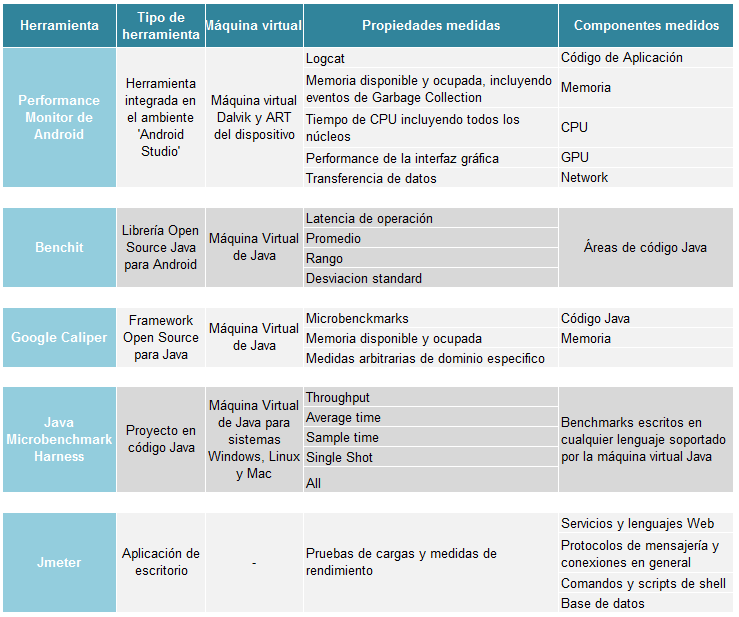
\includegraphics[scale=0.55]{C:/Users/usuario/Tesisworkspace/Tesis_Standalone/tesis/images/benchmarks_tools}
\par\end{centering}

\caption{Información resumida de herramientas de pruebas de performance para
aplicaciones Android y servicios Web.}
\label{tab:benchmarks-tools}
\end{table}



\section{Predicción de propiedades no funcionales con aprendizaje de máquina
\label{sec:Predicci=0000F3n-de-propiedades-no-funcionales-con-aprendizaje-de-m=0000E1quina}}

La predicción de propiedades no funcionales ha contribuido a los arquitectos
de software en la evaluación de sus sistemas durante la etapa de diseño,
y guiar las decisiones respecto a los componentes que deben integrarse
a la arquitectura del sistema de acuerdo a los requerimientos de calidad
esperados. Diferentes trabajos han recurrido al uso de técnicas de
aprendizaje de máquina para construir modelos de predicción de performance
y otros atributos de calidad dinámicos. Hutter, Xu y Hoos \citep{Hutter2014}se
han referido a estos modelos como modelos empíricos de performance
(\emph{EPM} por sus siglas en inglés) ya que requieren la recolección
de mediciones empíricas sobre los componentes. La principal aplicación
de estos modelos probablemente es el problema de selección de algoritmos,
introducido en 1976 por John R. Rice \citep{Rice1976}. Este problema
consiste en seleccionar el algoritmo, o configuración de algoritmo,
de un portafolio de alternativas que minimice el tiempo de respuesta,
según la instancia de datos de entrada. La predicción del tiempo de
respuesta ha sido abordada con éxito usando técnicas de aprendizaje
supervisado, principalmente de regresión \citep{Hutter2014}. En estos
trabajos, los datos empíricos de entrenamiento son obtenidos en contextos
de ejecución controlados, para enfocarse en la correlación entre la
propiedad a predecir y las propiedades de los parámetros de entrada
del componente o algoritmo. Una limitación de estos modelos es que
no generalizan la predicción de las propiedades de performance al
contexto de ejecución, es decir, no consideran características del
dispositivo y el ambiente de ejecución que influyen sobre el desempeño
del componente, como su capacidad de cómputo y la disponibilidad de
recursos. 

Este capítulo describe trabajos que inducen al desarrollo de una herramienta
capaz de generalizar cualquier característica propia del componente
de ejecución como así también del entorno donde se ejecuta para la
aplicación de la técnica de aprendizaje de máquina que resulte la
más adecuada para la predicción. Está organizado de la siguiente manera:
la sección \ref{sub:Predicci=0000F3n-de-precisi=0000F3n} presenta
tres estudios sobre algoritmos de optimización que abarcan la predicción
de otro de los indicadores más importantes, como lo es la precisión
y en la sección \ref{sub:Predicci=0000F3n-sobre-Servicios} presenta
dos estudios de propiedades dinámicas sobre Servicios Web. 


\subsection{Predicción de precisión sobre algoritmos de optimización. \label{sub:Predicci=0000F3n-de-precisi=0000F3n}}

Los modelos de predicción no sólo se utilizan para estimar el tiempo
de respuesta del desempeño de los componentes, sino también para estimar
otras propiedades. Mark Roberts, Adele Howe y Landon Flom \citep{Roberts07learnedmodels}
han construido dos modelos para la predicción del tiempo de respuesta
y para la probabilidad de éxito de diferentes algoritmos de planeamiento
utilizando técnicas de aprendizaje de máquina incluidas en la librería
Weka. Para el aprendizaje fueron utilizados 4726 benchmarks, problemas
o instancias para ejecutarse sobre 28 algoritmos de planeamiento conocidos.
Por cada algoritmo y cada problema se registra si un plan fue encontrado
(éxito) a través de los valores verdadero o falso y se registra el
tiempo (en segundos) requerido en completar la ejecución. Ya que cada
algoritmo define su propia forma en que un resultado es exitoso o
no, de forma automática obtienen las métricas de precisión porcentuales
sobre la salida. 

Otros autores (Mersmann; Bischl; Trautmann; Wagner; Bossek y Neumann
\citep{Mersmann_anovel}) predicen la optimalidad o razón de aproximación
de algoritmos para el problema del viajante utilizando una técnica
de regresión no lineal llamada \emph{MARS}, por sus siglas en inglés.
El modelo \emph{MARS} se aplicó con éxito para predecir la calidad
de aproximación del algoritmo de búsqueda local llamado 2-opt independiente
del tamaño de la instancia sobre la base de las características de
los casos generados con una precisión muy alta. Se cree firmemente
que debiera ser sencillo aplicar la misma metodología a otros algoritmos
y utilizar estos modelos para derivar una estrategia para el problema
de selección de algoritmos en el contexto de los problemas \ac{TSP}.

Finalmente, el trabajo desarrollado por los autores Beveridge, Givens,
Phillips y Draper \citep{Beveridge2009} se analiza la precisión de
tres componentes diferentes para el reconocimiento de rostros en imágenes,
utilizando una técnica de regresión lineal denominada GLMM, por Generalized
Linear Mixed Models. 


\subsection{Predicción sobre Servicios Web \label{sub:Predicci=0000F3n-sobre-Servicios}}

La predicción de propiedades dinámicas de servicios Web, como su tiempo
de respuesta, throughput y probabilidad de fallos, es más compleja
de abordar con respecto a componentes locales ya que depende del estado
de la infraestructura de red y el proveedor del servicio, que no se
puede monitorear desde el dispositivo cliente. Un enfoque ingenioso
para abordar este problema fue propuesto en el articulo de Zheng\citep{Zheng2013}.
En este trabajo, los autores se basan en la premisa de que las propiedades
de performance de los servicios Web varían respecto a características
del contexto como la ubicación geográfica y el momento del día y la
semana en el que se realiza una solicitud al servicio. De esta forma,
recolectan la información del consumo de servicios de múltiples clientes
alrededor del mundo para generalizar modelos de predicción. Este enfoque
es conocido como predicción colaborativa ya que los datos empíricos
de entrenamiento son brindados por múltiples nodos de manera distribuida.
Los autores llevaron a cabo un experimento a gran escala que involucró
más de 30 millones de invocaciones a servicios Web en más de 80 países,
por usuarios distribuidos en más de 30 países. La observación experimental
indica que diferentes usuarios pueden tener diferentes experiencias
de uso sobre el mismo servicio, influenciados por la conexión de red
y los ambientes heterogéneos entre usuarios y proveedores. Los datos
se encuentran disponibles públicamente y han sido utilizados en varios
trabajos para la construcción y comparación de modelos de performance
con diferentes técnicas de aprendizaje de máquina \citep{Albu2013}\citep{Kumar2015}. 
\acresetall


\chapter{Enfoque y Herramientas\label{chap:Enfoque-y-Herramientas}}

En este capítulo se describe el enfoque propuesto para extraer información
y conocimiento de un conjunto de características inherentes a componentes
de software y propiedades estáticas y dinámicas del dispositivo android
de ejecución para analizar las relaciones y dependencias y predecir
atributos no funcionales en base a dichas propiedades. Para el diseño
se hizo énfasis en la optimización combinada de los parámetros de
los algoritmos de aprendizaje automático. 

El enfoque plantea llevar a cabo la predicción de propiedades no-funcionales
mediante un proceso de aprendizaje de máquina a través de \emph{i})
la recolección de indicadores o mediciones tomados a partir de la
información provista de la ejecución de piezas de software, considerando
atributos de componentes, atributos inherentes al problema de entrada,
y atributos de la operación y resultados de la ejecución, y \emph{ii})
la construcción de modelos como un proceso interactivo con el usuario
a partir de la configuración inicial de los datos, la optimización
automática de los parámetros de acuerdo a las tasas de error arrojadas
por métricas de evaluación y el ajuste final del modelo a través del
análisis de las curvas de aprendizaje. 

Como soporte para el enfoque, se desarrollaron dos herramientas independientes
entre sí y diseñadas para efectuar el objetivo y conexión de las dos
fases propuestas. Por un lado, se desarrolló una herramienta denominada
\emph{Android Performance Testing and Prediction} cuyo diseño se adapta
fácilmente a la implementación de cualquier dominio computacional
del que se quiera obtener indicadores de desempeño. Al tratarse de
un framework implementado para el sistema Android, permite obtener
de manera directa los benchmarks del dispositivo de interés para el
análisis. Por otro lado, se desarrolló una herramienta standalone
denominada \emph{Nekonata} diseñada para brindar soporte al uso de
las funciones de cualquier librería que realice aprendizaje automático
y minería de datos escritas en lenguaje Java y que consiste en dos
fases, una primer etapa para la construcción del modelo a partir del
conjunto fuente de benchmarks mediante un proceso de automatización
de los algoritmos en complemento de información gráfica para la colaboración
interactiva del usuario y finalmente una segunda etapa de ajustes
al modelo teniendo en cuenta los efectos de overfitting y underfitting
consecuentes del entrenamiento. 

Estas cuestiones se describen en detalle de la siguiente manera. En
la sección \ref{sec:Aplicaciones-de-la} se enumeran algunos de los
usos prácticos de los modelos incluyendo aplicaciones de la propuesta.
Luego, en la sección \ref{sec:Etapas-del-m=0000E9todo} se profundiza
sobre las distintas etapas del enfoque y flujo de trabajo. En la sección
\ref{sec:Herramientas} se describen cada uno de los frameworks desarrollados,
presentando la herramienta para la recolección de datos en la subsección
\ref{subsec:Framework-de-medici=0000F3n} y finalmente, en la sección
\ref{subsec:Herramienta-de-entrenamiento} se presenta la herramienta
para la construcción de modelos evaluativos. 


\section{Aplicaciones de la propuesta \label{sec:Aplicaciones-de-la}}

Los problemas de clase NP - Completos están presentes en la mayoría
de ámbitos computacionales. Afortunadamente, en la medida que estos
problemas resultan difíciles de resolver frente a los peores casos
de entrada, se hace más factible resolverlos aún considerando problemas
de grandes instancias. 

Desafortunadamente, estos algoritmos pueden exhibir variaciones extremas
de ejecución a través de las instancias con distribuciones reales,
incluso, aunque la dimensión del problema se mantuviera constante,
la misma instancia puede requerir dramáticamente diferentes tiempos
de ejecución en función del algoritmo utilizado. Existe una escasa
comprensión teórica de las causas de esta variación. Durante la última
década, una cantidad considerable de trabajo ha intentado demostrar
cómo utilizar las técnicas de aprendizaje automático supervisado para
la construcción de modelos de regresión que proporcionen respuestas
aproximadas a esta pregunta en base a los datos de rendimiento del
algoritmo analizado, en otras palabras, podría creerse que es posible
predecir el tiempo que requerirá un determinado algoritmo para ejecutarse
bajo una entrada en particular construyendo un modelo de tiempo de
ejecución del algoritmo como una función de las características específicas
de cada instancia del problema. 

La construcción de tales modelos conocidos como \emph{modelos de actuación
empírica }(EPM por sus siglas en inglés) ha ido creciendo y motivada
debido a la utilidad que presentan frente a una gran variedad de contextos
prácticos. A continuación, se detallan algunos:
\begin{description}
\item [{Selección~de~algoritmos}] Como se ha tratado en algunos trabajos
\citet{Hutter2014}, los modelos de predicción son útiles para la
selección automática de algoritmos y la configuración en una variedad
de formas (un problema clásico de selección del mejor algoritmo entre
un determinado conjunto); a través de \ac{EPM} se logra predecir
el rendimiento de cada uno de estos algoritmos candidatos y mediante
un análisis comparativo, seleccionar el más apropiado considerando
la instancia del problema y las características del hardware. 
\item [{Ajustes~de~parámetros~y~configuración~automática~del~algoritmo}] \ac{EPM}
sirve a dos propósitos fundamentales, por un lado, modelar el comportamiento
o funcionalidad de un algoritmo parametrizado en base a la configuración
de tales parámetros, en cuyo caso se puede alternar entre el aprendizaje
del modelo y su uso para identificar configuraciones interesantes
para evaluar posteriormente. Por otro lado, se puede modelar el rendimiento
del algoritmo basado conjuntamente en las características de las instancias
del problema y la configuración de sus parámetros. Tales modelos pueden
utilizarse para ajustar los valores de tales parámetros y obtener
una mejor predicción basada en la instancia particular. 
\item [{Generación~de~benchmarks~fuertes}] Un modelo predictivo para
uno o más algoritmos se puede utilizar para establecer los parámetros
de los generadores de benchmarks existentes con el fin de crear instancias
asociadas al algoritmo particular. 
\item [{Obtener~una~visión~general~de~las~instancias~y~el~rendimiento~de~los~algoritmos}] \ac{EPM}
se puede utilizar para evaluar las características de la instancia
y los valores de los parámetros del algoritmo que más impactan en
el rendimiento. Algunos modelos son compatibles con este tipo de evaluaciones
directamente. Para otros modelos, existen métodos de selección de
atributos (características genéricas) para identificar un grupo más
reducido de entradas del modelo que son claves, y describen el rendimiento
del algoritmo casi tan bien como todo el conjunto de entradas. 
\item [{Selección~de~Servicio~y~composición}] Cuando varios servicios
web implementan la misma funcionalidad, los modelos de rendimiento
resultan ser un buen criterio para escoger el mejor candidato entre
ellos. Incluso en tiempo de ejecución, los proveedores de servicio
pueden cambiarse si las condiciones del contexto y los parámetros
de entrada se modifican. 
\item [{Programación~de~tareas~en~redes~móviles}] Suponiendo un conjunto
de tareas que deben asignarse entre un conjunto de dispositivos, los
modelos de rendimiento podrían obtener una medida exacta del tiempo
de respuesta que cada tarea requerirá sobre cada dispositivo con el
fin de minimizar el tiempo total de secuenciación de las tareas. 
\item [{Otros.}]~
\end{description}

\section{Etapas del método\label{sec:Etapas-del-m=0000E9todo}}

El enfoque propuesto se conceptualiza como un proceso de tres fases
complementarias. Este ciclo o flujo de trabajo da lugar a tres etapas
bien definidas por cada dominio o escenario de estudio, desde la obtención
de indicadores hasta la predicción de propiedades no funcionales en
entornos de aplicación. La figura \ref{fig:method-stages} muestra
un esquema conceptual del enfoque, cuyas etapas se describen a continuación:

\begin{figure}
\begin{centering}
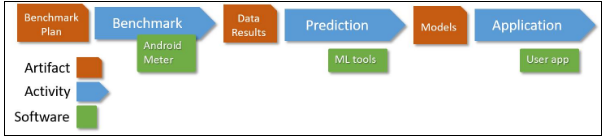
\includegraphics[scale=0.55]{C:/Users/usuario/Tesisworkspace/Tesis_Standalone/tesis/images/method-stages}
\par\end{centering}

\caption{Esquema conceptual del enfoque en fases. \label{fig:method-stages}}
\end{figure}



\subsection{Etapa recolección de datos }

\noindent El proceso comienza con la creación de datasets. Cada dataset
pertenece a un escenario o dominio diferente, del cual se extraen
todas las características que podrían influir sobre el desempeño del
componente. Durante la ejecución de cada servicio o pieza de software
se van realizando las mediciones o métricas sobre distintos aspectos
de la operación y registrando cada uno de estos benchmarks en un archivo
para su posterior análisis. A su vez, el proceso de recolección de
benckmarks involucra la ejecución de sub etapas, pudiendo requerir
el proceso algunas, o todas de las tareas que se detallan a continuación:
\begin{itemize}
\item Integración de componentes: A menudo se requiere la evaluación de
componentes de terceros, tanto de servicios Web como librerías instaladas,
de manera que deben ser integrados correctamente a la herramienta
para ser tratados como componentes. 
\item Selección de características del contexto: Mientras se realiza la
ejecución de los componentes, las propiedades no funcionales del dispositivo
móvil donde se llevan a cabo las operaciones, pueden ser capturadas
como indicadores. Realizar las mediciones en distintos modelos de
dispositivos móviles persigue la idea sobre la influencia de las capacidades
de cada modelo en las operaciones de ejecución. Ya que las predicciones
son realizadas sobre componentes de aplicaciones Android, la captura
de las carecterísticas estáticas y dinámicas son tomadas en cuenta,
para detectar relaciones entre éstas y los atributos a predecir de
los componentes.
\item Implementación de dominios: La evaluación de casos de estudios variables
en complejidad y características,que incluyen diferentes formatos
de componentes, son analizados con el fin de arrojar conclusiones
sobre la variación en el desempeño de las técnicas de regresión frente
a diferentes ambientes, analizar la calidad en el aprendizaje para
atributos no funcionales; cuánta mejora en la precisión significa
la aplicación de técnicas de regresión sobre problemas de complejidad
polinómica respecto a problemas NP, o la afectación en el tiempo de
respuesta de las operaciones sobre servicios remotos frente a servicios
locales, son algunas de las conclusiones que podrían desprenderse
del análisis. 
\item Generación de instancias de entrada: Se debe proveer una manera para
generar arbitrariamente instancias de un dominio particular, o la
capacidad para obtener instancias externamente a través de enlaces
o archivos. 
\item Selección de características de la entrada: Es posible obtener atributos
propios a la entrada del dominio, generalmente atributos que configuran
o sirven para generar una instancia. 
\item Ejecución de componentes y obtención de métricas: Los componentes
son ejecutados con las entradas generadas, tomando y registrando mediciones
sobre las características incorporadas además de las propiedades de
interés a predecir. De esta forma, los dataset pueden ser formados
por una cantidad variable y opcional de atributos en base a las características
que hayan sido elegidas para ser medidas. Este factor impacta en la
calidad del dataset creado, por lo tanto estudiar el comportamiento
que adoptan los datos y la distribución en el rango de valores, puede
servir de indicio para entender el desempeño de las técnicas. 
\end{itemize}

\subsection{Etapa aprendizaje}

A partir del conjunto de benchmarks obtenidos en la etapa anterior,
se aplican técnicas de aprendizaje de máquina para la extracción de
conocimiento de los datos. Tal conocimiento se refleja mediante la
construcción de modelos predictivos que mejor se ajustan a la generalización
de la información mediante un proceso de entrenamiento, optimización
y evaluación de los mismos. El proceso de aprendizaje requiere indefectiblemente
de un conjunto de datos de entrenamiento volcado en un archivo, un
atributo de ese conjunto a predecir y un conjunto de algoritmos que
aplican técnicas de regresión sobre los datos. Actualmente, hay herramientas
que proveen estos algoritmos incluyendo toda la funcionalidad necesaria
para este proceso, y que son fácilmente integrables a cualquier desarrollo.
Además, el aprendizaje está conformado por varias etapas o sub procesos.


\paragraph{Configuración de las técnicas }

Las técnicas de regresión representan modelos matemáticos cuyas funciones
involucran diferentes parámetros de configuración. La variabilidad
en estos valores permite ajustar las preferencias del algoritmo y
consecuentemente, la obtención de modelos de calidad diferente. Por
lo tanto, el desafío principal de esta parte de la etapa es encontrar
los valores apropiados para cada uno de los parámetros, teniendo como
base, el conocimiento sobre el efecto que el parámetro causa en el
algoritmo. Al obtener la mejor configuración de una técnica, para
un dataset y un atributo particular, se facilita la comparación simultánea
de todas las técnicas disponibles a través de las métricas de evaluación
y en consecuencia seleccionar la más óptima. 




\paragraph{Construcción de modelos }

La construcción de modelos predictivos es un proceso que inicia con
el entrenamiento de los datos, continúa opcionalmente con un proceso
de validación y concluye con una evaluación del error cometido en
las estimaciones frente a los datos reales del entrenamiento.

La implementación de los casos de estudio enfatizan la predicción
de la precisión en las respuestas y el tiempo de ejecución de los
componentes considerando a ambas métricas esenciales al momento de
seleccionar el/los componente/s más adecuado/s para un propósito particular,
dadas ciertas entradas, componentes posibles, restricciones y parámetros
deseados.

La fase de entrenamiento de este proceso utiliza las mediciones ya
obtenidas en la etapa anterior y a partir del atributo que se desea
predecir, el algoritmo va definiendo la función de regresión para
encontrar las relaciones entre los atributos del dataset y el atributo
a predecir. Esta fase concentra el mayor porcentaje del tiempo computacional
y uso de memoria, y varía de acuerdo a la complejidad o simplicidad
de cada técnica en particular. 


\paragraph{Evaluación de modelos}

Una vez concluida la fase de entrenamiento, la calidad del modelo
obtenido debe ser analizada para determinar la medida en que el modelo
será capaz de generalizar cualquier entrada de dataset futura. La
noción sobre el desempeño del modelo tiene lugar a partir de métricas
ya definidas para modelos de regresión, que capturan distintamente
el error de predicción e incluyen el coeficiente de correlación para
conocer el grado de interdependencia de las variables. 

A pesar que el objetivo de alcanzar estimaciones bajas en error es
importante, el análisis no debe centralizarse únicamente en la minimizacíón
del error en las predicciones, sino que debe estar dirigido por las
curvas de aprendizaje. Las curvas de aprendizaje permiten observar
gráficamente el modo en que el modelo se ajusta a los datos de entrenamiento,
evidenciando efectos de sobreajuste, el modelo sólo será bueno para
ese dataset en particular, o efectos de baja adaptación, debido principalmente
a que no se cuenta con los suficientes datos para enseñar al modelo. 


\subsection{Etapa predicción }

Finalmente, se pretende utilizar estos modelos de predicción en entornos
de aplicación que permitan la selección del componente más adecuado
en base a un conjunto de propiedades del problema de entrada, las
propiedades internas del dispositivo en el cual se llevará a cabo
la ejecución, y un conjunto de restricciones que deben satisfacerse,
a través de un proceso automatizado que determine al usuario la opción
más favorable evitando la ejecución individual de cada componente. 


\section{Herramientas\label{sec:Herramientas}}

El trabajo presentado conforma dos de las tres fases propuestas para
el enfoque global del desarrollo. La primer fase se lleva a cabo en
un framework particular para la medición de propiedades de componentes
Android que será detallada en la sección \ref{subsec:Framework-de-medici=0000F3n}.
La segunda fase para la construcción de modelos predictivos a través
de técnicas de aprendizaje de máquina se desarrolla en una segunda
herramienta la cual será detallada en la sección \ref{subsec:Herramienta-de-entrenamiento}. 


\subsection{Framework de medición para Android\label{subsec:Framework-de-medici=0000F3n}}


\subsubsection*{Enfoque general}

\emph{Android Performance Testing and Prediction} es un framework
diseñado para realizar mediciones de performance de componentes ejecutados
bajo el sistema Android. Es una herramienta de testing que permite
ejecutar diferentes piezas de software y evaluar propiedades influyentes
y características del entorno de ejecución. 

La herramienta cuenta con el soporte necesario para adaptarse a cualquier
dominio informático y exportar las mediciones correspondientes en
archivos de formato \ac{CSV}, mediciones que servirán de fuente para
herramientas de predicción a través de técnicas de aprendizaje de
máquina. 


\subsubsection*{Objetivos}

El rendimiento de los componentes de ejecución (algoritmos, servicios
Web, procesos ejecutándose en segundo plano, etc.) dependen de varios
factores: el contexto de ejecución donde el componente está funcionando,
los parámetros de entrada que requiere el componente de la operación
y su implementación interna. Sin embargo, al utilizar componentes
de terceros es posible desconocer el modo en el que fueron implementados,
actuando como cajas negras a los desarrolladores móviles, que sólo
conocen sus interfaces de aplicaciones, pero no su trabajo interno. 

Para elaborar un análisis del rendimiento, técnicas de aprendizaje
automático sobre los datos recogidos empíricamente pueden ser utilizados
para construir modelos de predicción del tiempo de ejecución del componente,
como una función de los parámetros de entrada y las características
específicas del contexto de ejecución: configuración de algoritmos,
selección de servicios, planificación de trabajos, por citar algunos
ejemplos. 


\subsubsection*{Enfoque}

El enfoque principal de esta herramienta está centrado en dos propiedades:
el tiempo de respuesta y la precisión de los resultados. 

El tiempo de respuesta refiere al tiempo total que demanda un componente
en ejecutar una operación o tarea, es decir, el tiempo para responder
a una solicitud con una entrada determinada. Por otro lado, la precisión
es una medida que evalúa la calidad de los resultados o salida de
un componente y tiene diferentes significados semánticos dependiendo
de la funcionalidad requerida, por ejemplo, en problemas de clasificación,
se toma el concepto de precisión como la medida estadística de la
eficacia de un clasificador, la precisión está relacionada a la identificación
o exclusión correctamente de una condición. En problemas de optimización,
también conocido como optimalidad, la precisión es una relación entre
la solución de salida obtenida y la solución óptima conocida. 

Para construir un modelo de predicción del tiempo de respuesta sobre
un componente particular, se deben considerar dos variables al momento
de evaluar, un conjunto acerca de las características del contexto
de ejecución, por ejemplo, núcleos de CPU, tipo de red, etc. y otro
conjunto acerca de las características de la entrada en particular,
por ejemplo, en tamaño expresado en bytes. 

Del mismo modo se construye un modelo de predicción de precisión sobre
un componente, como en la mayoría de los casos esta medida no depende
de las características del contexto en el que se ejecuta, el modelo
respondería a una función dependiente de las entradas del problema.


\subsubsection*{Componentes}

El análisis de rendimiento que se propone en esta herramienta se basa
en entidades de software individuales de ejecución que proveen servicios
a través de una interfaz específica. De aquí en más, estas entidades
se denotarán componentes. 

\begin{figure}
\begin{centering}
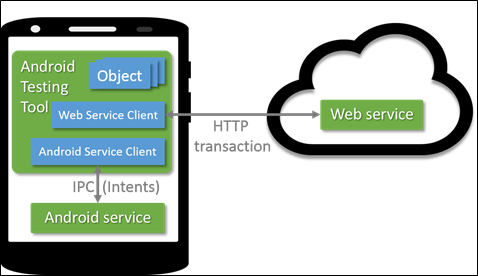
\includegraphics[scale=0.55]{C:/Users/usuario/Tesisworkspace/Tesis_Standalone/tesis/images/android-component}
\par\end{centering}

\caption{Esquema conceptual de componentes Android considerados. \label{fig:android-component}}
\end{figure}


En la figura \ref{fig:android-component} se pueden observar los tres
tipos de componentes generalizados por la herramienta para obtener
los resultados de mediciones adecuados, incluyendo servicios Web y
servicios específicos de la plataforma Android, mientras que para
toda pieza de software remanente los componentes son tratados simplemente
como objetos Java. Las instancias de objetos hacen referencia a cualquier
componente residente en el espacio de memoria de una aplicación, el
componente específico para servicios web incluye cualquier componente
remoto fuera del dispositivo y accedidos a través de protocolos de
comunicación Web, como \ac{HTTP}. Por último el componente específico
para servicios Android incluye cualquier proceso ejecutado en segundo
plano residente en el mismo dispositivo y accedidos a través de objetos
Intent (como único mecanismo de comunicación entre procesos del sistema
Android). 


\subsubsection*{Diseño e implementación}

El proyecto \emph{Android-Testing-Tool} constituye el modelo base
del framework \emph{Android-Performance-Testing-and-Prediction} para
llevar a cabo el proceso de medición de propiedades de cualquier tipo
de componente. Además, se proveen dos proyectos a modo de ejemplo
demostrando el modo de uso de el framework. El proyecto \emph{Evaluation-of-Face-Detection-Services}
fue diseñado para obtener mediciones sobre servicios que ofrecen reconocimiento
facial y el proyecto \emph{Examples-Android-Testing-Tool} fue diseñado
para dominios de problemas NP, incluyendo a problemas de la clase
P y NP - Completos. 

A continuación se expone en la figura \ref{fig:TestingTool-Diagram}
los principales factores que han servido de guía para el diseño del
proyecto base \emph{Android-Testing-Tool}. 

\begin{figure}
\begin{centering}
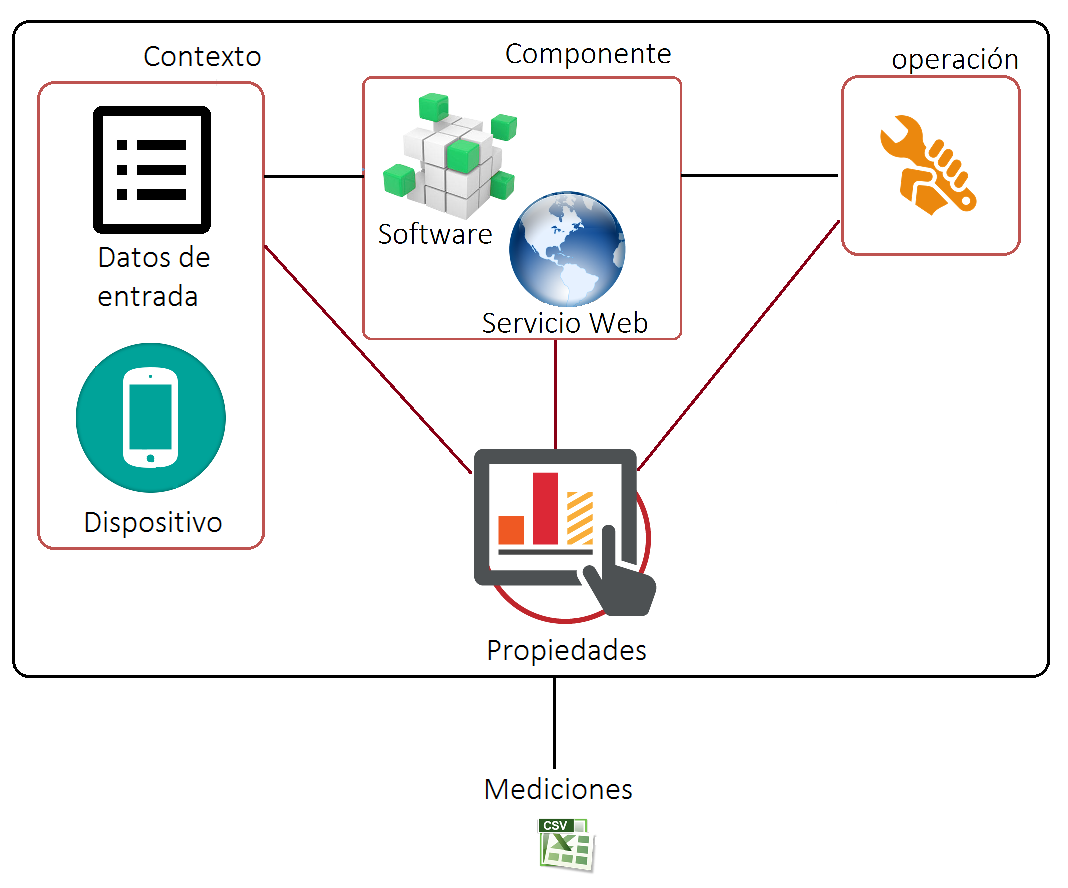
\includegraphics[scale=0.1]{C:/Users/usuario/Tesisworkspace/Tesis_Standalone/tesis/images/TestingTool-Diagram}
\par\end{centering}

\caption{Diagrama estructural de la herramienta template \emph{Android Testing
Tool}.\label{fig:TestingTool-Diagram}}


\selectlanguage{english}%
\selectlanguage{english}%
\end{figure}


La forma de organizar diferentes modelos de evaluación se realiza
a través de la creación de planes de prueba, que se configuran y posteriormente
se ejecutan para obtener un archivo de formato \ac{CSV} con el resultado
de todas las mediciones incorporadas al plan de pruebas. La herramienta
implementa por defecto un objeto llamado \emph{TestPlan} que define
una ejecución sistemática de las operaciones y métricas sobre ellos.
Básicamente, un modelo de plan de pruebas se compone de un conjunto
posible de componentes, un conjunto posible de objetos de entrada,
y un conjunto posible de métricas para realizar las mediciones, dando
la posibilidad de configurar estas propiedades a los requerimientos
deseados. Una vez configurado y ejecutado el plan de pruebas, los
resultados con las mediciones son almacenados en un objeto denominado
\emph{Results} y los datos son exportados a un archivo de formato
\ac{CSV} para su posterior procesamiento. 

La herramienta utiliza una representación simplificada de los componentes,
pudiendo ser éstos servicios Web o simplemente piezas de software
implementadas por el programador. Los parámetros que recibe son dos
objetos del tipo \emph{Input} y \emph{Output}, siendo éstos, instancias
de objetos que representan la entrada y salida del problema respectivamente.
Cada uno de los componentes asociados a un problema específico ejecutan
una operación o tarea a través de la llamada al método \emph{execute}
del componente. Esta operación es responsable de evaluar la ejecución
de la instancia de entrada en el componente y retornar un objeto de
salida o respuesta del problema. Tanto \emph{Input} como \emph{Output}
son dos conceptos abstractos que representan instancias reales del
problema. Una instancia de entrada puede encapsular no sólo los parámetros
requeridos para realizar la ejecución del componente, sino la configuración
de los mismos. Por otro lado, una instancia de salida encapsula la
respuesta o resultado de esa operación. Durante la ejecución del plan
de pruebas (ejecución de cada uno de los componentes asociados), se
evalúan los indicadores que fueron configurados como métricas en el
plan. Se distinguieron cuatro tipos de métricas en función del elemento
de medición, determinando el parámetro que recibe: 
\begin{enumerate}
\item Métricas globales sobre características estáticas del contexto: cualidades
del entorno de ejecución que se mantienen estáticas (sin cambio) durante
el plan de pruebas, por ejemplo, modelo del dispositivo, arquitectura
de la CPU, cantidad de núcleos de CPU, tamaño de memoria, etc. 
\item Métricas generales sobre características de la entrada: atributos
inherentes al dominio del problema, por ejemplo, en el problema de
detección de rostros algunas características podrían ser el nombre
de imagen, tamaño o contraste, formato de archivo, etc.
\item Métricas generales del componente: propiedades del componente como
el nombre, su ubicación, etc.
\item Métricas de operación: Son medidas que actúan sobre la ejecución del
componente, por lo cual distinguen en tres tipos diferentes:

\begin{itemize}
\item Características de la salida: características o métricas obtenidas
a partir del resultado de la operación, por ejemplo el tamaño de la
salida, la precisión de la misma, etc.
\item Características dinámicas del contexto: características del entorno
de ejecución que pueden variar de una operación a otra, como el uso
de CPU, el número de procesos en ejecución, tipo de conexión, ubicación
del dispositivo, etc. 
\item Características de desempeño: medidas de interés sobre el rendimiento
que varían de una operación a otra, como el tiempo de respuesta, el
consumo de batería, operaciones ejecutadas con éxito o con error,
etc.
\end{itemize}
\end{enumerate}
El framework de medición ha sido diseñado para soportar distintos
dominios sobre los cuáles tomar las medidas deseadas. Por el momento
sólo implementa dos tipos de dominios: por un lado, problemas clásicos
del tipo NP para el análisis del desempeño de diferentes algoritmos
de resolución y por otro lado, aplicaciones de propósito general,
en este caso, aplicaciones que ofrecen reconocimiento facial para
la evaluación de diferentes servicios que ofrecen esta misma funcionalidad,
como ya ha sido anticipado. Los problemas de complejidad NP se contemplan
bajo un proyecto individual llamado \emph{Examples-Android-Testing-Tool}
para la evaluación de desempeño de distintos algoritmos considerando
dos aspectos fundamentales: tiempo (aproximación del número de pasos
de ejecución que emplea el algoritmo) y espacio (aproximación de la
cantidad de memoria utilizada). Los problemas implementados pertenecen
tanto a la clase P como a la clase NP-Completos. Por otro lado, el
objetivo de la incorporación de dominios que implican el uso de servicios
remotos se basa en la idea de automatizar el testeo continuo de uno
o varios servicios, en este caso, aplicaciones que ofrecen reconocimiento
facial, teniendo en cuenta las características que estos pueden proveer
y aquellas que el usuario de la aplicación desee considerar, de esta
manera determinar el servicio más adecuado (según el contexto) para
la ejecución de una tarea. Este dominio ha sido diseñado a través
de un proyecto individual bajo el nombre de \emph{Evaluation-of-Faces-Detection-Services}.
Este proyecto se implementó como un modelo básico y genérico sobre
el proceso de detección de rostros. Tal proyecto conforma una estructura
general para almacenar y acceder a todos los atributos posibles que
cualquier servicio que brinde la funcionalidad de detección de rostros
pudiera ofrecer. Es importante destacar algunos detalles sobre los
componentes, entradas y métricas que fueron tomados en cuenta en el
diseño del proyecto. Cada componente representa un servicio particular,
cuya performance es evaluada y analizada; en base a los parámetros
de configuración que acepta cada uno de estos servicios, se generan
diferentes instancias de componentes posibles, un servicio que admite
dos variables de configuración, por ejemplo, da lugar a cuatro tipos
de componentes como producto de la combinación de opciones configurables
posibles. En cuanto a las entradas del dominio, pueden añadirse al
plan de pruebas a través de archivos o de manera estática especificando
la ruta de cada imagen. Finalmente, fueron consideradas métricas respecto
al proceso u operación (rostros correctamente detectados, rostros
detectados y Tiempo de respuesta) y respecto a la imagen de entrada
(contraste, entropía, formato, intensidad promedio, cantidad de rostros
en la imagen, cantidad de pixeles de la imagen, tamaño y nombre).
Respecto al servicio, sólo se registra el nombre del mismo. 


\subsection{Herramienta de entrenamiento y evaluación de modelos\label{subsec:Herramienta-de-entrenamiento}}

El eje que ha guiado el diseño de la herramienta ha sido el brindar
soporte para el uso de cualquier librería que ofrezca aprendizaje
de máquina a través de la implementación de todos los conceptos involucrados
como objetos independientes a los cuales adaptar las funcionalidades
de las librerías. La herramienta \emph{Nekonata} lleva a cabo dos
tipos de procesos en el desarrollo de sus funciones, procesos automatizados
y procesos que requieren la colaboración del usuario con el fin de
mejorar los resultados a partir de vistas gráficas sobre el comportamiento
y características de los modelos y además, para incluir en el proceso
el interés y criterio del usuario. 

El enfoque y objetivo de la herramienta se concluyen en dos etapas,
una fase de entrenamiento de modelos y una fase de evaluación y mejora
de los mismos. 

En la figura \ref{fig:prediction-tool} se muestran las vistas iniciales
de la herramienta , presentación y configuración de datos. 

\begin{figure}
\begin{centering}
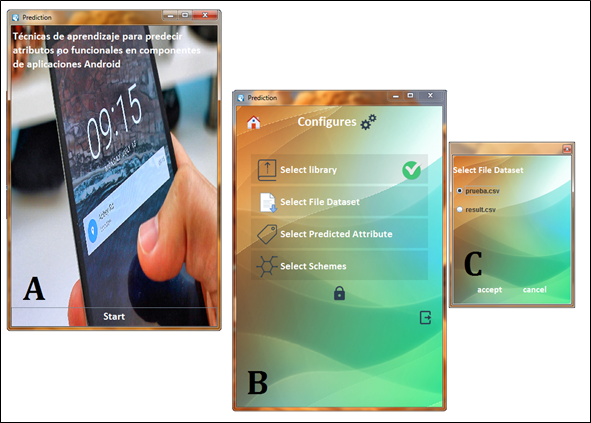
\includegraphics[scale=0.55]{C:/Users/usuario/Tesisworkspace/Tesis_Standalone/tesis/images/prediction-tool}
\par\end{centering}

\caption{Captura de pantalla de la herramienta: (A) Presentación, (B) Configuración
de datos, (C) Menú de selección de opciones.\label{fig:prediction-tool}}
\end{figure}



\subsubsection{Entrenamiento de modelos}

En esta sección se brindará un enfoque global y expresarán las consideraciones
de los conceptos relacionados al proceso de entrenamiento. Posteriormente,
se describe en detalle el flujo de desarrollo del proceso. Estos conceptos
han sido el eje del diseño de la herramienta. A continuación, se presenta
un listado de los objetos tratados: 


\subsubsection*{Librerías}

Al día de hoy se han implementado bibliotecas que realizan aprendizaje
automático en múltiples lenguajes de programación. A pesar de la gran
variación que existe entre unos y otros, el uso de técnicas de aprendizaje
de máquina se rige bajo los mismos conceptos: durante la etapa de
entrenamiento, un conjunto de datos que servirán como base de datos
del proceso y una lista de algoritmos categorizados según realicen
una función de regresión o clasificación (distinción que lleva a cada
biblioteca definir los tipos de atributos numéricos y categóricos),
finalmente durante la etapa de evaluación, es necesario el uso de
métricas o indicadores matemáticos para evaluar la calidad del clasificador.
Estos principios permiten generalizar el término \emph{librería} independizando
la implementación específica de cada biblioteca añadida al sistema. 

La herramienta Nekonata utiliza la biblioteca Weka, una plataforma
de software para el aprendizaje automático y la minería de datos escrito
en Java y desarrollado en la Universidad de Waikato y popularmente
conocida ya que contiene una extensa colección de técnicas para preprocesamiento
de datos y modelado. 


\subsubsection*{Base de datos}

Los archivos dataset usados para el entrenamiento, a menudo son vistos
como una grilla de valores cuyas columnas representan cada una de
las características del dominio comúnmente denominadas clases o atributos
y cuyas filas denominadas instancias representan cada uno de los ejemplos
del escenario de estudio. Bajo estas consideraciones, a nivel conceptual
existe un objeto único como dataset que obtiene los datos a través
de un proceso de parseo del archivo fuente a los objetos correspondientes
de la librería utilizada, generalizando toda funcionalidad requerida
mediante el acceso a la representación de los atributos e instancias. 


\subsubsection*{Instancias}

Tal como se adelantó anteriormente, cada dataset está formado por
un conjunto de ejemplos tomados de un dominio en particular. Cada
ejemplo constituye una instancia individual del problema representada
por un conjunto de dos valores, el nombre del atributo y su respectivo
indicador.


\subsubsection*{Modelos}

La herramienta Nekonata está orientada al aprendizaje supervisado
de predicción mediante funciones de regresión e incluye la técnica
adaptada de agrupamiento a través de cluster como alternativa. Ambos
casos fueron diseñados para incorporar los algoritmos que se deseen
asegurando el correcto uso de sus funciones.


\subsubsection*{Parámetros}

Los algoritmos de aprendizaje automático se rigen bajo fórmulas matemáticas
que a menudo incluyen constantes o coeficientes cuyo valor incide
directamente en la calidad y desempeño del clasificador. Algunos algoritmos
no tienen parámetros adicionales más que los atributos del dominio,
otros en cambio, tienen parámetros simples o complejos. Un parámetro
simple es aquel conformado por un único valor y un parámetro complejo
aquel constituido por una serie de valores, en la mayoría de casos
se trata de algoritmos internos del algoritmo principal, tal es el
caso de la función Kernel que utilizan los algoritmos de vectores
de soporte. 


\subsubsection*{Optimización}

Los algoritmos pueden aplicarse utilizando los valores por defecto
de los parámetros sin embargo pueden variarse conjuntamente para adaptarse
mejor a los datos de entrenamiento y producir modelos predictivos
más adecuados. Un proceso de optimización define rangos de valores
válidos para cada uno de los parámetros admitidos y ejecuta a través
de un proceso evaluativo, la combinación cruzada de cada opción, evaluando
cada alternativa posible. Como resultado, se obtiene la mejor de todas
las configuraciones para el algoritmo en cuestión.

La herramienta Nekonata considera la optimización de algoritmos de
regresión, clusterers y funciones kernel. 

Las consideraciones mencionadas anteriormente son el punto de partida
en el mecanismo de aprendizaje. El proceso de entrenamiento de modelos
(Figura \ref{fig:prediction-workflow}) básicamente lleva a cabo la
configuración de todos los datos requeridos para ejecutar los algoritmos
clasificadores y obtener, posteriormente los modelos. Estos datos
están directamente afectados por la biblioteca de aprendizaje automático
que se use por lo que se dispondrá de diferentes opciones de selección
variando entre una librería y otra. Esta disposición dio lugar a un
flujo determinado en el orden de las actividades. 

\begin{figure}
\begin{centering}
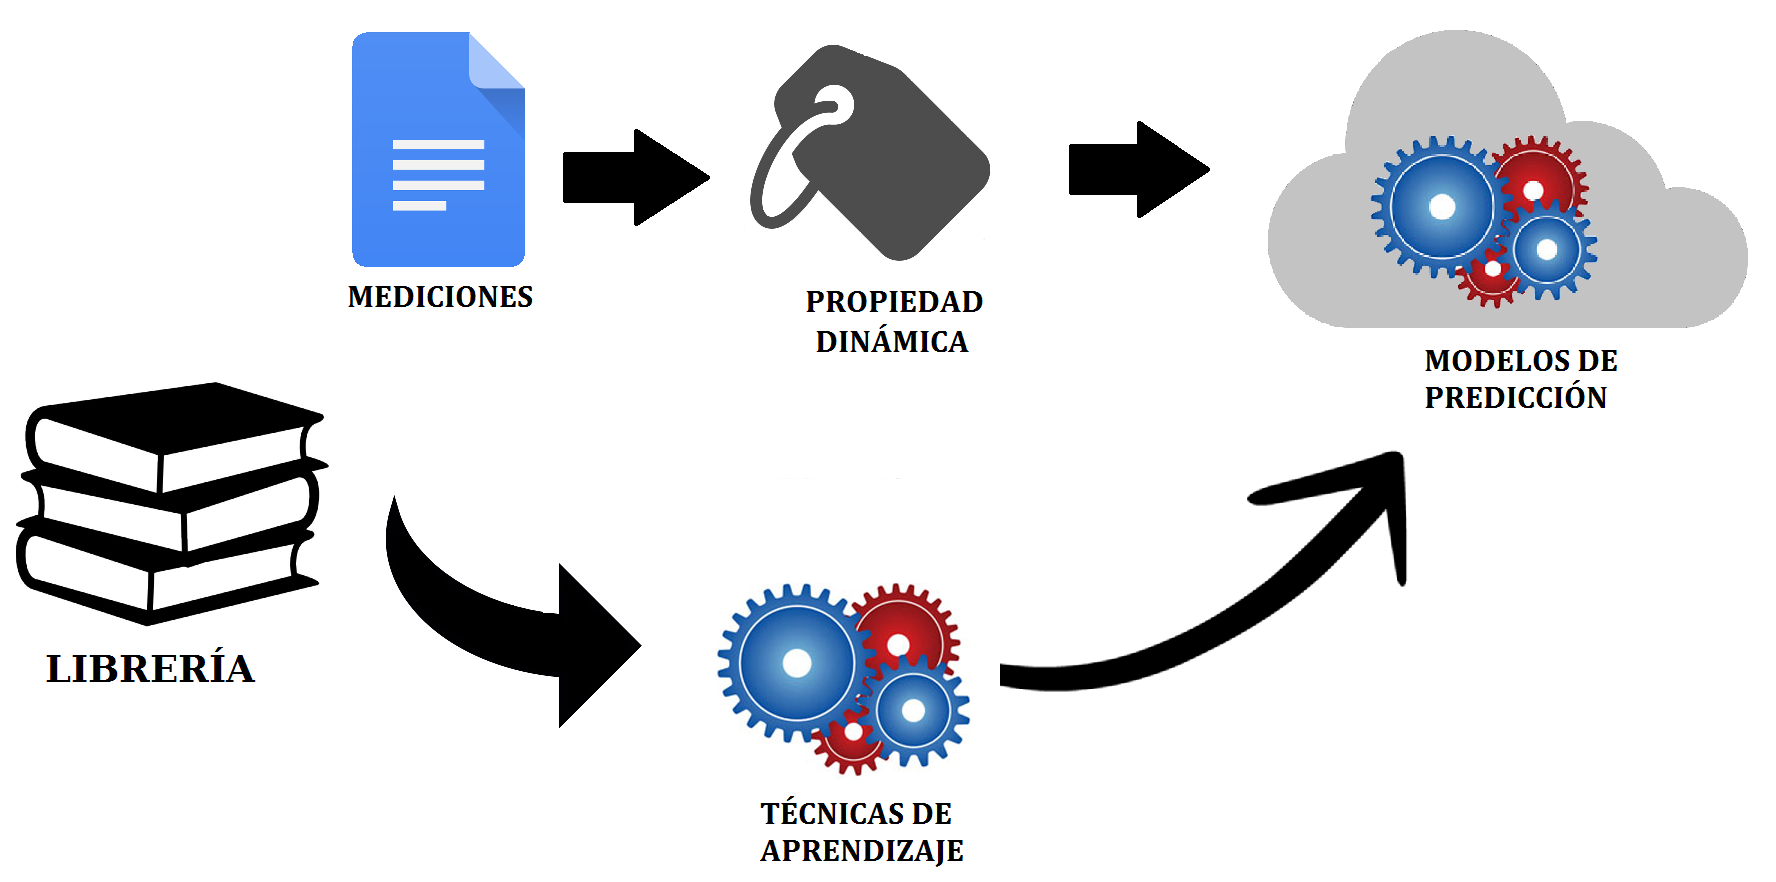
\includegraphics[scale=0.55]{C:/Users/usuario/Tesisworkspace/Tesis_Standalone/tesis/images/prediction-workflow}
\par\end{centering}

\caption{Diagrama de flujo del proceso de entrenamiento de modelos.\label{fig:prediction-workflow}}
\end{figure}


La selección de la librería de aprendizaje automático es el punto
de partida condicionando el resto de los datos configurables. Luego,
al seleccionar el archivo fuente con los benchmarks medidos en formato
CSV, a través de un proceso de parseo se obtiene el archivo comúnmente
llamado dataset adaptado al formato de instancias de la librería.
Con este nuevo formato se extraen los atributos para seleccionar aquel
que se pretenda predecir y junto con la selección de algoritmos se
inicia la optimización de los mismos. 

Los algoritmos de aprendizaje se habilitan al momento de elegir la
librería a utilizar ofreciendo sólo aquellos que la librería dispone.
La multi selección de clasificadores brinda la posibilidad al usuario
de elegir los algoritmos de mayor preferencia o interés para optimizar
en ese momento evitando el proceso de optimización de todos los clasificadores
lo cual significaría un ahorro en el uso de los recursos computacionales. 

Finalmente, como resultado de esta etapa se obtiene el conjunto de
clasificadores seleccionados cuyas configuraciones son las más favorables
para los datos de entrenamiento 


\subsubsection{Evaluación de modelos}

En esta sección se detallarán las consideraciones y los enfoques generales
del proceso de evaluación y métricas de error. También, se especificará
el flujo de las actividades llevadas a cabo para calificar el desempeño
del clasificador y realizar ajustes de ser necesario. 


\subsubsection*{Evaluación}

El dataset de origen, también denominado conjunto de datos de aprendizaje
o entrenamiento, es utilizado para obtener el modelo predictivo que
generalice esos datos adecuadamente. El término generalizar hace referencia
a obtener una función que se ajuste a los datos en cuanto minimice
el \emph{error empírico} que es el error producido por el algoritmo. 

El proceso de evaluación, entonces, debe utilizar nuevos datos de
entrada (preferentemente distintos al conjunto de entrenamiento) y
predecir la salida a partir de éstos arrojando ciertamente una tasa
de error en la predicción hecha por el clasificador. Existen dos métodos
clásicos de evaluación en base al origen de los datos usados para
la validación de modelos. El más sencillo resulta de utilizar los
mismos datos que fueron usados para la fase de entrenamiento. El método
restante conocido bajo el nombre de validación cruzada (\emph{Cross
validation}) tiene una metodología más compleja. 

El método de validación cruzada utiliza un coeficiente \emph{K} de
repetición y división; los datos de entrada se dividen en \emph{K}
subconjuntos, utilizando uno de ellos como dato de prueba y el resto
(\emph{K-1}) como datos de entrenamiento. El proceso es repetido durante
\emph{K} iteraciones, con cada uno de los posibles subconjunto de
datos de prueba. Finalmente se calcula la media aritmética de los
resultados de cada iteración para obtener un único resultado. Los
resultados de la evaluación son contemplan mediante un conjunto de
indicadores que se describirán más adelante. Nekonata implementa ambos
métodos e incluye la funcionalidad necesaria para acceder a todos
los valores predictivos. 


\subsubsection*{Métricas}

Las métricas usadas para la evaluación de los algoritmos simplemente
son fórmulas matemáticas o composición de ellas que involucran únicamente
a dos variables, los valores reales del dominio y los valores predictivos.
En la herramienta se ha implementado el conjunto de indicadores más
popular brindando, conjuntamente, la posibilidad de utilizar las métricas
ofrecidas por cada biblioteca incorporada. También, se han definido
e incorporado cuatro características globales asociadas a las métricas
para brindar soporte a otras funcionalidades. Toda métrica \emph{i})
brinda algún tipo de información, acerca del error de predicción o
estadísticas o atributos de los datos; \emph{ii}) tiene una representación
particular de los indicadores, los valores pueden estar normalizados
en una escala del 0 al 1, expresados en porcentajes o simplemente
adaptados a la escala de los datos; \emph{iii}) definen por su naturaleza
un requerimiento minimo o maximo de su indicador y \emph{iv}) son
aplicables a un tipo de función ya sea regresión o clasificación. 

Con el fin de extremar las mejoras y asegurar que el modelo resultante
sea el más favorable para el conjunto de datos usados en el entrenamiento
el proceso de evaluación de modelos fue dividido en dos fases. Luego
de la etapa de entrenamiento, los algoritmos clasificadores optimizados
son expuestos a una serie de métricas dispuestos de manera tal que
permita visualizar las diferencias de desempeño entre clasificadores
con la misma métrica considerada. Esta vista es un recurso ofrecido
al usuario para decidir aquel modelo que a su criterio tenga mejor
calidad a través de la comparación simultánea y continuar mejorando
el modelo elegido a partir del análisis de los efectos de underfit
y overfit. 


\subsubsection*{Fase 1: Comparación de modelos}

La optimización de un algoritmo clasificador para obtener la configuración
más apropiada para el conjunto de datos es conveniente,sin embargo,
resulta más útil aplicar un proceso de optimización a un conjunto
de algoritmos candidatos para luego analizar cuál de ellos es el que
mejor generaliza los datos. La comparación entre clasificadores se
realiza por medio de métricas que arrojan una estimación acerca del
error de predicción, es decir, una medida que refleja la diferencia
entre los datos reales del dominio y los valores predichos por el
algoritmo. Es conveniente trasladar el análisis a la mayor cantidad
de métricas posibles, ya que un mismo indicador podría arrojar valores
cercanos entre un algoritmo y otro favoreciendo equivocadamente a
uno de ellos, error que podría notarse al compararlos simultáneamente
con otras métricas. La metodología de operación de esta fase se muestra
en la figura \ref{fig:models-comparison-workflow}. 

Nekonata hace foco en este detalle y ofrece al usuario una vista de
imágenes con los indicadores medidos de cada algoritmo seleccionado
por el usuario para aplicar el proceso de optimización y elegir, posteriormente,
el que resulte más adecuado. La información gráfica complementaria
que se brinda, detalla los algoritmos representados por medio de barras
y agrupados en categorías separadas de acuerdo a cada métrica a modo
de facilitar la comparación. Adicionalmente las barras se colorean
en dos tonos diferentes para acentuar, por cada métrica, los clasificadores
que significarían las mejores opciones para ese indicador. 

\begin{figure}
\begin{centering}
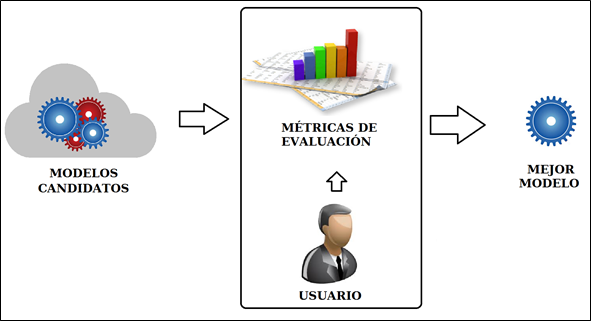
\includegraphics[scale=0.55]{C:/Users/usuario/Tesisworkspace/Tesis_Standalone/tesis/images/models-comparison-workflow}
\par\end{centering}

\caption{Diagrama de flujo de la fase de comparación de modelos. \label{fig:models-comparison-workflow}}
\end{figure}


La disposición de todas las métricas de evaluación se han distribuido
en imágenes dispares para agruparlas según la clase de información
que representan, ya sean indicadores del error de predicción o características
sobre los datos. En el primer caso también se distinguen entre aquellas
métricas interpretadas a valores normalizados entre cero y uno y métricas
a valores de escala del atributo. De esta forma se agrupan en conjuntos
los indicadores proclives a compararse mutuamente como puede observarse
en la figura \ref{fig:screenshot-errors}. 

El aporte del usuario se incorporó para personificar el interés y
criterio para determinar los indicadores más significativos para basar
la elección del modelo más favorable. De esta manera, cada usuario
puede basar su elección analizando y comparando los indicadores que
a su criterio son más relevantes. 

\begin{figure}
\begin{centering}
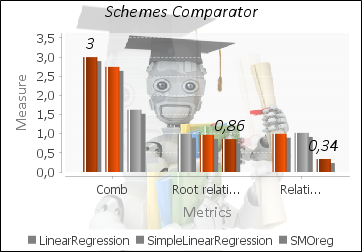
\includegraphics[scale=0.55]{C:/Users/usuario/Tesisworkspace/Tesis_Standalone/tesis/images/screenshot-errors}
\par\end{centering}

\caption{Captura de pantalla de la vista de indicadores sobre el error de predicción
normalizados.\label{fig:screenshot-errors}}
\end{figure}



\subsubsection*{Fase 2: Ajustes al modelo}

A través del uso de métricas se adquiere una idea estimativa del desempeño
del clasificador frente al conjunto de datos de entrenamiento, sin
embargo, podría resultar útil conocer el comportamiento general del
algoritmo, contrastando cada uno de los valores reales del atributo
clase con los valores predichos por el clasificador, y obtener así
una vista exacta de la manera en que el clasificador se ajusta a los
datos (Figura \ref{fig:screenshot-error-curve}). 

Este recurso es usado en la herramienta como un gráfico de dos líneas
continuas de distinto color para representar el conjunto de datos
de entrenamiento y el conjunto de datos predichos. Cada punto del
dominio corresponde a cada instancia y la unión entre puntos sólo
se realiza con fines ilustrativos. 

\begin{figure}
\begin{centering}
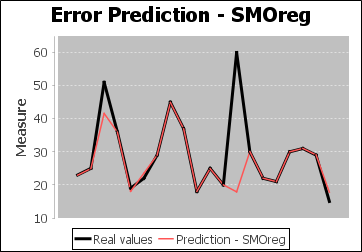
\includegraphics[scale=0.55]{C:/Users/usuario/Tesisworkspace/Tesis_Standalone/tesis/images/screenshot-error-curve}
\par\end{centering}

\caption{Captura de pantalla de la vista del error de predicción. \label{fig:screenshot-error-curve}}
\end{figure}


El análisis del error de predicción es la base para comprender la
calidad del modelo construido hasta el momento aunque no es el único
objetivo, ya que la vista permite extraer conocimiento de cómo se
comporta el conjunto de datos de entrenamiento, existencia de valores
extremos, la variación de los valores tomados, entre otros. Es un
recurso gráfico para complementar la información que se le brinda
al usuario y encaminarlo a un correcto proceso de ajuste del modelo. 

\begin{figure}
\begin{centering}
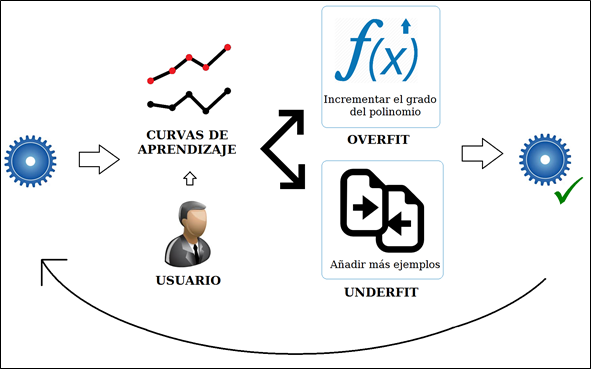
\includegraphics[scale=0.55]{C:/Users/usuario/Tesisworkspace/Tesis_Standalone/tesis/images/adjustment-workflow}
\par\end{centering}

\caption{Diagrama de flujo de la fase de ajuste.\label{fig:adjustment-workflow}}
\end{figure}


El flujo de desarrollo de esta fase se planteó como un proceso de
carácter opcional e iterativo para el usuario. Se puede optar simplemente
por almacenar el modelo elegido durante la etapa de comparación anterior
o repetir las veces que se desee un procedimiento de análisis de las
curvas de aprendizaje del modelo y las acciones consecuentes para
reparar los posibles efectos, como se muestra en la figura \ref{fig:adjustment-workflow}.


A continuación se explicará el funcionamiento de la fase brindando
una visión general del planteamiento de las curvas de aprendizaje
con las respectivas consideraciones que se tuvieron en cuenta y la
manera en que se ha incluido la participación del usuario para la
transformación del conjunto de datos. 


\paragraph*{Curvas de aprendizaje}

Las curvas de aprendizaje se componen por dos líneas de puntos representadas
en el mismo plano cartesiano. Ambas líneas grafican el error de predicción
utilizando los dos métodos de evaluación conocidos, aplicando el conjunto
de entrenamiento o el método de validación cruzada.Las curvas de aprendizaje
implementadas por la herramienta son mostradas en la figura \ref{fig:learning-curves}

El procedimiento considera una cantidad de instancias determinadas,
cantidad que se incrementa en un factor constante para aplicar el
modelo y calcular el error cuadrático medio, es decir, la diferencia
cuadrática entre el valor real del atributo y el predicho por el modelo. 

En un primer paso, la herramienta toma en cuenta las primeras cinco
instancias, luego las primeras diez, las primeras quince y así sucesivamente
para conformar cada punto del dominio cuyo valor de ordenada es el
error cuadrático, error añadido en la herramienta como parte del conjunto
de métricas consideradas. Por cuestiones de facilitar la vista se
impuso un límite en los valores del dominio reducido en trescientas
(300) instancias en caso de que el conjunto de entrenamiento supere
dicha cantidad. 




\paragraph*{Opciones para el usuario}

En Nekonata se han incluido dos acciones posibles para reparar, en
caso de evidenciar, los efectos de overfit o underfit del modelo.
Estas dos acciones no son mutuamente excluyentes de manera que el
usuario puede elegir libremente alguna o ambas acciones a la vez,
sin embargo, la herramienta le recomienda la acción que debería tomar
en caso de un efecto u otro. Ambas acciones realizan una transformación
en la base de datos, cuando el usuario decide incorporar nuevas instancias
o ejemplos del dominio introduce un archivo el cuál es parseado al
formato conocido por la librería de uso y es unido al conjunto original
siendo ahora, el nuevo conjunto de datos. Por otro lado, cuando el
usuario decide aumentar el grado del polinomio que emplea el modelo,
elige un número entre uno y cuatro para modificar este polinomio y
así, añadir a la base de datos los nuevos atributos originarios del
nuevo polinomio completo para ese grado. 


\subsubsection{Diseño e implementación}

A pesar que la herramienta fue pensada para la predicción de componentes
de android,se desarrolló como una aplicación de escritorio debido
a la limitación del hardware de los dispositivos móviles para ejecutar
los procesos de optimización que consumen un gran porcentaje de recursos
computacionales. Esta implementación desvincula la herramienta de
medición con la herramienta de entrenamiento y evaluación de modelos,
permitiendo la ejecución independiente entre ambas por lo que el puente
de comunicación entre ellas es la correspondencia entre la salida
de la primer herramienta con la entrada de la segunda; la herramienta
de medición crea archivos de formato \ac{CSV}, los cuales serán usados
en la herramienta como el conjunto de datos fuente para el entrenamiento. 


\subsubsection*{Entorno y tecnologías}

Para la implementación del framework Nekonata se utilizó el entorno
de desarrollo Eclipse cuyo lenguaje de programación es Java. El proyecto
ha sido configurado con la versión \ac{JDK} 1.7 y \ac{JRE} 1.8 y
además, se han incorporado tecnologías de terceros para el entorno
las cuáles cumplen distintos roles en la herramienta. 

Para el diseño de la interfaz gráfica se utilizó mayormente la librería
SWING de java incorporada en el \ac{JDK} aunque también se incluyeron
componentes de la librería nativa AWT. La principal ventaja de la
librería SWING es brindar una interfaz adaptada a cada sistema operativo
sin necesidad de cambio de código, es decir independiente a la plataforma.
Complementariamente se incorporaron las dos siguientes librerías:
\emph{jgoodies-forms-1.8.0.jar} y \emph{miglayout15-swing.jar}

Por otro lado, para la creación de vistas para el usuario se incorporó
la biblioteca gráfica de Java JFREECHART que facilita la creación
de varios tipos de gráficos profesionales, en el caso de la herramienta
se han utilizado los gráficos de barras y lineales para representar
la información requerida por el usuario. Esta biblioteca ha sido elegida
por brindar objetos de alta calidad y ofrecer una extensa gama de
funciones para reforzar y mejorar la información mostrada en los gráficos.
Se utilizó la versión 1.0.19 de la biblioteca en complemento con la
librería JCOMMON en la versión 1.0.23. 

Respecto al uso de técnicas de aprendizaje de máquina, actualmente
existen muchas tecnologías y frameworks que proveen esta funcionalidad
para utilizar en entornos Java, sin embargo, como se ha adelantado
anteriormente en la herramienta sólo se incluyó la biblioteca \emph{Weka}
en la versión 3.8 y se añadió también un paquete para la optimización
de parámetros perteneciente a la misma librería denominado MULTISEARCH
en su versión más actual del mes de agosto del 2016. 


\subsubsection*{Diseño}

Considerando todo lo anteriormente descrito, el concepto principal
de la herramienta fue la extensibilidad de la misma desde todos los
enfoques posibles. Esto significa que la herramienta pudiera aceptar
diferentes tipos de librerías de aprendizaje de máquina, datasets,
modelos de regresión, parámetros y métricas; lo que conlleva a un
gran grado de abstracción de las clases que conforman la aplicación
y, por lo tanto, se consideró importante la asociación de mismas,
para un entendimiento mayor de parte de un nuevo desarrollador.

La finalidad de la etapa de implementación fue un buen framework de
trabajo para el futuro desarrollo de modelos, librerías y métricas.
Si bien la herramienta sólo trabaja con Weka actualmente y la mayoría
de su funcionalidad es enteramente parser , se considera que el grado
de abstracción es lo bastante elevado para poder soportar la finalidad
deseada.

Aplicando los conceptos teóricos antes presentados, se exponen a continuación
los paquetes y las clases principales que componen el desarrollo de
Nekonata. 


\paragraph*{Databases}

Como ya se mencionó anteriormente se desea poder administrar, leer
y escribir datasets de forma dinámica y segura. Para esto, se creó
una estructura para almacenar cada individuo (instancia) con una estructura
\emph{Hashtable}, con los nombres de los atributos como claves de
los valores numéricos que representan a cada uno de ellos.

Asimismo, se desarrolló un conjunto para representar los datasets
ya que son estos las bases de los modelos, del aprendizaje y del framework,
tomando como entrada un csv y creando la base de datos necesaria para
el correcto funcionamiento de la aplicación. 

\begin{figure}
\begin{centering}
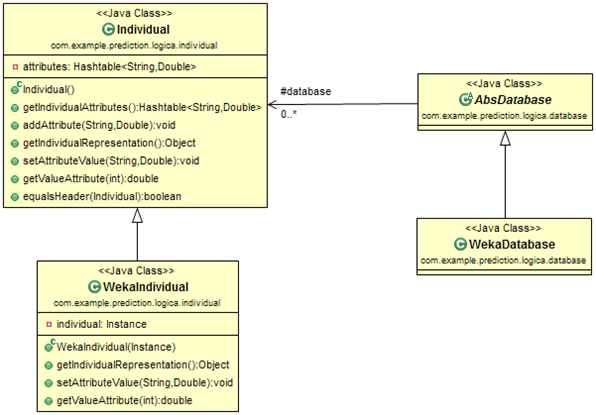
\includegraphics[scale=0.55]{C:/Users/usuario/Tesisworkspace/Tesis_Standalone/tesis/images/database-class-diagram}
\par\end{centering}

\caption{Diagrama de clases de las bases de datos implementadas\label{fig:database-class-diagram}}
\end{figure}



\paragraph*{Modelos}

Los modelos que la herramienta presenta son de tipo regresivo pero
no necesariamente son modelos intrínsecamente predictivos y por eso
el framework presenta una división clara entre modelos regresivos
y clasificadores (siempre considerando que estos últimos se utilizan
para la regresión).

\begin{figure}
\begin{centering}
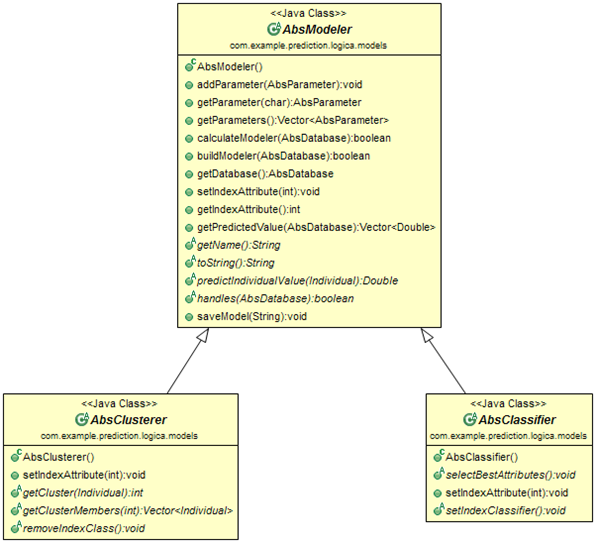
\includegraphics[scale=0.55]{C:/Users/usuario/Tesisworkspace/Tesis_Standalone/tesis/images/modelers-class-diagram}
\par\end{centering}

\caption{Diagrama de clases de los modelos base implementados.\label{fig:modelers-class-diagram}}
\end{figure}


A partir de esto, implementando los métodos abstractos presentados,
se pueden incluir cualquier método de clasificación requerido, siempre
considerando importante que retorne un valor denso. Actualmente, los
modelos implementados son los presentados en la sección \ref{subsec:Funciones-contempladas}.

\begin{figure}
\begin{centering}
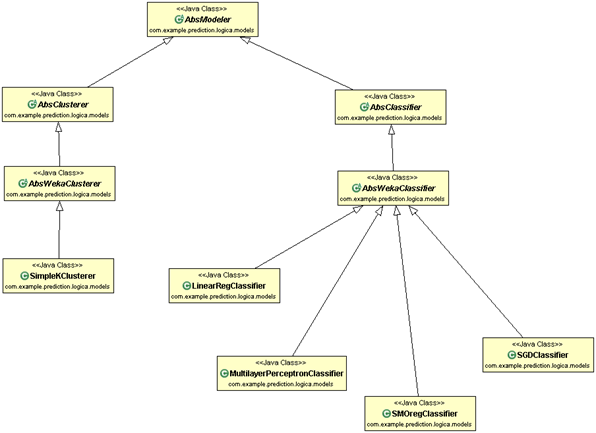
\includegraphics[scale=0.55]{C:/Users/usuario/Tesisworkspace/Tesis_Standalone/tesis/images/all-modelers-class-diagram}
\par\end{centering}

\caption{Diagrama de la relación entre los modelos implementados.\label{fig:all-modelers-class-diagram}}
\end{figure}


Como se puede apreciar en la figura \ref{fig:all-modelers-class-diagram}
, se realizó una abstracción intermedia considerando la librería Weka.
Esto se debe principalmente al comportamiento en común que tenían
dichos modelos, pero no es mandatoria dicha abstracción al agregar
una nueva librería o al agregar nuevos modelos. 

Ya que el diseño fue impulsado por la necesidad de abstracción e independencia
de las librerías subyacentes, se considera importante la posibilidad
de que en un futuro cualquier desarrollador pueda incorporar modelos
implementados de forma particular. 


\paragraph{Parámetros}

Para implementar los modelos, la iniciativa fue modelar el concepto
teórico que los rige: funciones. Como ya fue explicado, las funciones
están moldeados por variables y parámetros. Las variables son aquellos
atributos modelados por la Hashtable en la clase individuo. Debido
a los modelos considerados en el apartado anterior, los parámetros
(o las constantes de una función) fueron modeladas en dos partes:
\begin{enumerate}
\item Parámetros simples: Son aquellos que sólo tienen un valor numérico
y que tiene un valor único en la función. Rigen en funcionamiento
del método de aprendizaje y determinan la calidad y finalidad que
tendrán los mismos. Estos tipos de parametros se utilizan en todo
el core de modelos ya que son la idea fundamental de cualquier función
matemática. 
\item Parámetros kernel: Son funciones matemáticas que se emplean en las
\ac{SVM}. Estas funciones son las que le permiten convertir lo que
sería un problema de clasificación no lineal en el espacio dimensional
original, a un sencillo problema de clasificación lineal en un espacio
dimensional mayor. Debido a que estas son funciones dentro de los
modelos, es conveniente el modelado de las mismas de forma particular.
\end{enumerate}
Observando ambos puntos, se puede apreciar una composición de parámetros
ya que las funciones se conforman por parámetros simples y los parámetros
kernel son funciones internas. Esto se puede observar en la figura
\ref{fig:parameters-class-diagram} . 

\begin{figure}
\begin{centering}
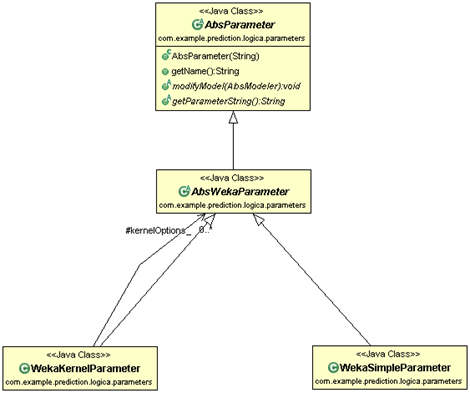
\includegraphics[scale=0.55]{C:/Users/usuario/Tesisworkspace/Tesis_Standalone/tesis/images/parameters-class-diagram}
\par\end{centering}

\caption{Diagrama de clases de los parametros implementados\label{fig:parameters-class-diagram}}
\end{figure}



\paragraph{Métricas}

Otra parte importante de la implementación de la herramienta es la
capacidad de la misma de cuantificar y valorizar los modelos obtenidos.
Las mismas ya vienen implementadas por la librería Weka, pero considerando
la finalidad de abstraer comportamiento, las mismas fueron parseadas
y se crearon nuevas clases.

\begin{figure}
\begin{centering}
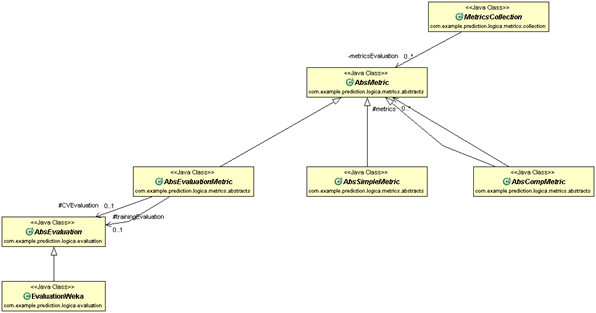
\includegraphics[scale=0.55]{C:/Users/usuario/Tesisworkspace/Tesis_Standalone/tesis/images/metrics-class-diagram}
\par\end{centering}

\caption{Diagrama de clases de las métricas implementadas.\label{fig:metrics-class-diagram}}
\end{figure}


La implementación presentada surge a partir de la forma de implementación
que tiene la librería weka. La misma presenta una clase que representa
la relación entre los valores reales que presenta la base de datos
y los valores calculados por el modelo. Sin embargo, la librería presenta
la particularidad de solo calcular métricas de los modelos que la
misma toma como de regresión. Así, el Simple K clusterer quedaría
excluido de este grupo y, por lo tanto, no podría ser valorado. La
implementación planteada permite que este modelo quede a la altura
de los otros presentados y que, si se desea, se pueden crear nuevas
métricas sin tener la clase \emph{AbsEvaluation} que represente esta
relación. Sólo sería necesario crear la métrica heredando de \emph{AbsSimpleMetric}
e implementar la forma de cálculo requerida.


\paragraph*{Optimización}

El paquete que se procede a explicar es implementado principalmente
considerando la función que proviene de Weka, permitiendo la prueba
de varios valores para los parámetros sin necesidad de pruebas constantes,
apuntando a una mejor y más rápida optimización del modelo. Puede
omitirse dicha implementación si se desea agregar un nuevo modelo,
pero es conveniente la explicación del mismo para futuras adaptaciones
de modelos de weka que se quieran agregar o de librerías que tengan
esta posibilidad también. 

La idea del paquete de optimización es que, de forma transparente
para el usuario de la aplicación, el modelo consiga adaptarse a la
base de datos analizada. Esto permite que la aplicación Nekonata pueda
adaptarse a grandes rangos de valores objetivo. Como ya se dijo anteriormente,
no es un paquete necesario en la aplicación ya que los parámetros
pueden ser puestos de forma fija en un modelo, pero esto restringe
el rango y las posibilidades del mismo. 

Los optimizadores cumplen la función de probar valores para los parámetros
y se quedan con aquellos que minimizan el grado de error del modelo.
Asimismo, cabe destacar que Weka proporciona dos tipos de optimizadores.
Los primeros son los simples, que consideran cada parámetro del modelo
desde un valor al otro. Los segundos son los kernels y prueban valores
no solo para los parámetros propios de los modelos sino para los parámetros
que conforman los kernels. 

\begin{figure}
\begin{centering}
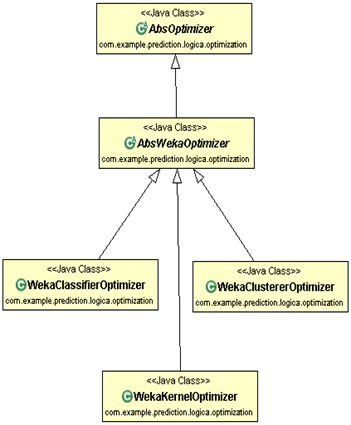
\includegraphics[scale=0.55]{C:/Users/usuario/Tesisworkspace/Tesis_Standalone/tesis/images/optimizer-class-diagram}
\par\end{centering}

\caption{Diagrama de clases de los optimizadores implementados.\label{fig:optimizer-class-diagram}}
\end{figure}



\paragraph*{Cómo agregar clases nuevas}

Todo lo anteriormente planteado se mantiene coherente y de forma congruente
gracias a la clase librería y lo que conlleva agregarla a la aplicación. 

\begin{figure}
\begin{centering}
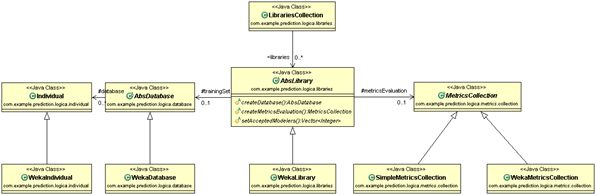
\includegraphics[scale=0.55]{C:/Users/usuario/Tesisworkspace/Tesis_Standalone/tesis/images/library-class-diagram}
\par\end{centering}

\caption{Diagrama de clases de las librerias y las relaciones con los otros
objetos.\label{fig:library-class-diagram}}
\end{figure}


Al crear la librería, y como se ve en el diagrama de clases, se deben
implementar dos métodos que devuelven dos conceptos principales. Por
un lado, un objeto de tipo Database que ya se explicó anteriormente.
Por el otro, un objeto MetricsCollection. Este último representa el
conjunto de métricas que sirven para valorizar los modelos. 

Ya implementado se provee el conjunto \emph{SimpleMetricsCollection}
que permiten valorizar cualquier modelo, ademas del \emph{WekaMetricsCollection}
que sólo contiene la metricas basadas en el \emph{WekaEvaluation}. 

La última función que se debe implementar de forma ineludible retorna
un vector de constantes. Estas constantes deben estar declaradas en
la clase \emph{Config.Modeler} con el formato: 

\fbox{\begin{minipage}[t]{1\columnwidth}%
\begin{center}
Nombre a mostrar en la aplicación: constante 
\par\end{center}%
\end{minipage}}

Las mismas declaran los modelos que son aceptados por la liberia.
Esto se hace a modo de índice para los modelos y, al momento de utilizar
la herramienta, las clases de los modelos sean creadas al momento
de ser seleccionadas. Esto se permite implementando la última función: 

\lstinline[language=Java,basicstyle={\footnotesize}]!public abstract Vector<AbsModeler> createModelers(Vector<Integer> selectedModels, int index);!

Esta última función crea la relación entre la constante con las clases
que se deben crear para representar a los modelos. 

\begin{figure}
\begin{centering}
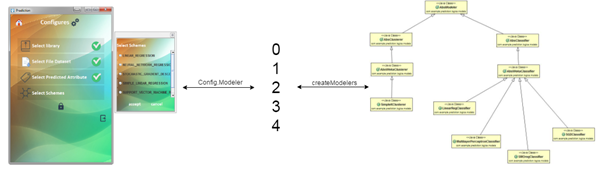
\includegraphics[scale=0.55]{C:/Users/usuario/Tesisworkspace/Tesis_Standalone/tesis/images/config-correlation}
\par\end{centering}

\caption{Diagrama conceptual de la configuración que presenta la herramienta\label{fig:config-correlation}}
\end{figure}



\subsubsection{Formato de los resultados\label{subsec:Formato-de-los}}

La herramienta devuelve como resultado un archivo en formato TXT almacenando,
por un lado, los valores resultantes de los parámetros fundamentales
de cada técnica y, por otro lado, la descripción del modelo construido.
La herramienta genera un archivo por cada técnica elegida por el usuario
para optimizar, en la dirección especificada en la configuración bajo
el nombre de la técnica. La figura \ref{fig:linear-regression-result}
permite una descripción gráfica de lo expresado anteriormente, donde
detalla A) los parámetros, B) Nombre del modelo y C) la función definida
para el atributo de predicción. 

\begin{figure}[H]
\begin{centering}
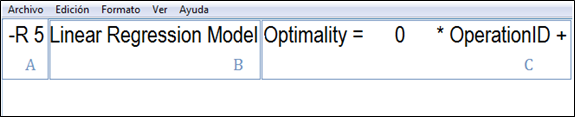
\includegraphics[scale=0.55]{C:/Users/usuario/Tesisworkspace/Tesis_Standalone/tesis/images/linear-regression-result}
\par\end{centering}

\caption{Ejemplo de resultado del modelo ‘Linear Regression’. \label{fig:linear-regression-result}}
\end{figure}


La manera en que los datos son expuestos al usuario no representa
un formato compatible para cualquier herramienta sobre aprendizaje
de máquina, esto se debe a que no existe actualmente, un formato estándar
para almacenar los modelos, y esta discrepancia entre las herramientas
disponibles exige un seteo manual de las técnicas por cada evaluación
que se realice
\acresetall
\chapter{Evaluación\label{chap:Evaluaci=0000F3n}}

En este capitulo se presenta la evaluación del enfoque propuesto con
el objetivo de analizar el desempeño de las técnicas de aprendizaje
de máquina utilizadas para predecir propiedades no-funcionales en
dispositivos móviles. Con este fin, se crearon tres casos de estudio
sobre los que se construyen y evalúan modelos de predicción.

El capítulo se organiza de la siguiente manera: en la sección \ref{sec:Metodolog=0000EDa-de-Evaluaci=0000F3n}
se detalla el proceso de evaluación propuesto. En las secciones \ref{subsec:Escenario-4:-Multiplicaci=0000F3n},~\ref{subsec:Escenario-1:-Algoritmos}~y~\ref{subsec:Escenario-2:-Servicios}
se presentan los escenarios de estudio considerados, brindando una
descripción de los componentes involucrados, las mediciones obtenidas
y los modelos de predicción construidos y evaluados. Los resultados
y discusión son expuestos en la sección \ref{sec:Analisis-y-discusi=0000F3n}
para analizar el desempeño de las técnicas de regresión sobre cada
caso de estudio. Finalmente en la sección \ref{sec:Conclusiones}
se presentan las conclusiones del capítulo. 


\section{Proceso de Evaluación\label{sec:Metodolog=0000EDa-de-Evaluaci=0000F3n}}

El proceso de evaluación, ilustrado en la Figura~\ref{fig:Proceso-de-evaluaci=0000F3n},
consiste en aplicar el enfoque sobre diferentes propiedades y grupos
de componentes, y evaluar los modelos de predicción con diferentes
métricas para analizar el desempeño de las distintas técnicas de aprendizaje
incluidas en la herramienta.

\begin{figure}
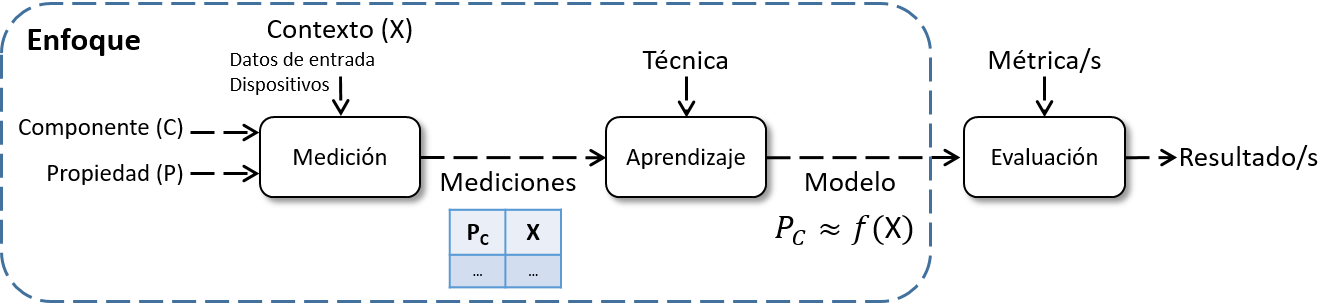
\includegraphics[scale=0.6]{images/Proceso-de-evaluacion}

\caption{Proceso de evaluación\label{fig:Proceso-de-evaluaci=0000F3n}}
\end{figure}


La calidad de los modelos será evaluada a través de dos métricas
que computan de forma distinta el error de predicción. Cada modelo
$f$ es construido por una técnica \emph{$T$} (regresión lineal,
red neuronal, etc.) que se aplica sobre un dataset de mediciones para
predecir una propiedad $P$ (tiempo de respuesta, precisión) de un
componente $C$. El proceso de evaluación consiste en tomar el conjunto
de mediciones usado para el aprendizaje de modelos de predicción y
utilizarlos para validar estos modelos a través las métricas de evaluación. 

Para un análisis más profundo sobre las distintas técnicas y su desempeño,
se usaron tres escenarios o casos de estudio de distintos dominios:
algoritmos para multiplicación de matrices, algoritmos para el problema
del viajante, y componentes para detección de rostros en imágenes.
Cada escenario comprende un conjunto de componentes y datos de entrada
a partir de lo cual se obtiene un dataset de mediciones. En todos
los escenarios se considera el tiempo de respuesta como propiedad
a medir y predecir. En el segundo y tercer caso de estudio, se considera
adicionalmente como propiedad la optimalidad o precisión en el resultado
arrojado por el componente.

El cuadro \ref{tab:Especificaciones-de-los-1} presenta la lista de
dispositivos sobre los que se han realizado las pruebas, con sus características
mas relevantes.

\begin{table}[H]
\begin{doublespace}
\begin{centering}
\resizebox{1\textwidth}{!}{%
\begin{tabular*}{20cm}{@{\extracolsep{\fill}}|c|c|c|c|c|}
\hline 
{\large{}Dispositivo} & {\large{}Frecuencia de CPU} & {\large{}Nucleos de CPU} & {\large{}Memoria RAM} & {\large{}Sistema Operativo}\tabularnewline
\hline 
{\large{}Lenovo K3 Note} & {\large{}1.7Ghz} & {\large{}Octa-Core} & {\large{}2GB} & {\large{}Android 5.0}\tabularnewline
\hline 
{\large{}Samsung Galaxy S3} & {\large{}1.4 Ghz, } & {\large{}Quad-Core} & {\large{}1GB} & {\large{}Android 4.3}\tabularnewline
\hline 
{\large{}Samsung Galaxy S4} & {\large{}1.9Ghz} & {\large{}Quad-Core} & {\large{}2GB} & {\large{}Android 4.2.2}\tabularnewline
\hline 
{\large{}Samsung Galaxy S5} & {\large{}2.5Ghz} & {\large{}Quad-Core} & {\large{}2GB} & {\large{}Android 4.4.2}\tabularnewline
\hline 
{\large{}Samsung Galaxy S6} & {\large{}2.1Ghz} & {\large{}Octa-Core} & {\large{}3GB} & {\large{}Android 5.0}\tabularnewline
\hline 
\end{tabular*}}
\par\end{centering}
\end{doublespace}

\caption{Características de los dispositivos móviles utilizados.\label{tab:Especificaciones-de-los-1}}
\end{table}



\subsection{Métricas de evaluación\label{subsec:M=0000E9tricas-de-evaluaci=0000F3n}}

Existe una gran cantidad de métricas por las cuales pueden evaluarse
y compararse los modelos de regresión. Todos los indicadores comparan
los valores reales con sus estimaciones, pero lo hacen de una manera
ligeramente diferente. 

\emph{\ac{MAE}} es el promedio del error absoluto (diferencia entre
los valores predichos y los observados), e indica cuán grande es el
error que puede esperarse de la predicción. Al tratarse de una métrica
basada en el error medio puede subestimar el impacto de errores grandes
pero infrecuentes. Si el análisis se centra demasiado en la media
arrojará conclusiones precipitadas, por lo tanto para ajustar errores
grandes y raros, se calcula el error cuadrático medio (\ac{RMSE}).
La ecuación de la métrica \ac{RMSE} es:

\[ \sqrt{\frac{1}{N}\sum_{i=1}^{N}{f_i-y_i}^2}
\]

La misma nos permite llegar a una medida del tamaño del error que
da más peso a los errores grandes e infrecuentes que la media. 

El coeficiente de correlación de Pearson es una medida de la relación
lineal entre dos variables aleatorias cuantitativas, independientemente
de la escala de medida de las mismas. El coeficiente de correlación
(\ac{CC}) es analizado en conjunto con el indicador \emph{\ac{RMSE}}
ya que existe una estrecha relación entre ambos. Por ejemplo, si \emph{\ac{CC}}
es 1, \emph{\ac{RMSE}} debe ser 0, ya que todos los puntos se encuentran
en la línea de la función de regresión; cuanto más cercano sea el
valor de \emph{\ac{CC}} a 1 o -1, más próximos son los valores observados
a la línea de predicción, y por tanto menor será el error absoluto
reflejado en \emph{\ac{RMSE}}. La fórmula de CC entre dos variables
\emph{x} e \emph{y} se define como:

\[
\frac{n\sum x_{i}y_{i}-\sum x_{i}\sum y_{i}}{\sqrt{n\sum x_{i}^{2}-(\sum x_{i})^{2}}\sqrt{n\sum y_{i}^{2}-(\sum y_{i})^{2}}}
\]



\subsection{Parámetros de configuración de las técnicas\label{subsec:Par=0000E1metros-de-configuraci=0000F3nde}}

La obtención de un modelo de calidad tiene lugar a partir de la optimización
de los parámetros de configuración de la técnica de regresión. Estos
parámetros pueden tomar distintos valores adaptándose a condiciones
particulares de los datos, generando modelos mas precisos que otros.
El Cuadro \ref{tab:Par=0000E1metros-de-configuraci=0000F3n} presenta
la lista completa de parámetros de configuración de cada técnica,
el valor por defecto adoptado para cada una y el rango de valores
con el cual se busca el modelo de mayor precisión. 

\begin{table}[H]
\begin{centering}
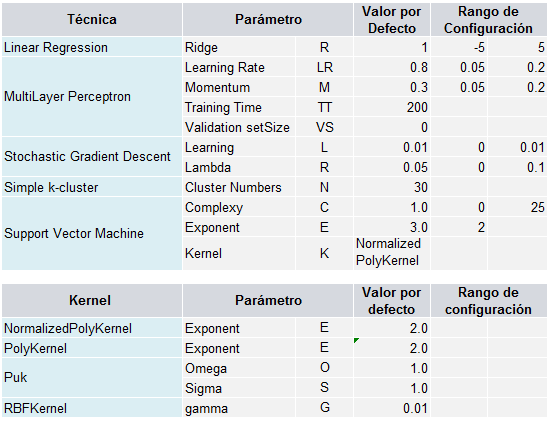
\includegraphics[scale=0.5]{images/configuration-parameters}
\par\end{centering}

\caption{Parámetros de configuración de las técnicas de regresión \label{tab:Par=0000E1metros-de-configuraci=0000F3n}}
\end{table}


El proceso de optimización de las técnicas utiliza el rango de configuración
establecido para iterar en pasos tomando valores intermedios y evaluando
la calidad del modelo generado con tales configuraciones. Los resultados
se comparan entre sí para determinar la mejor configuración para un
dataset y propiedad a predecir particular. 

Los rangos para cada técnica se establecieron tras un análisis de
la influencia de estos valores sobre los datos. Los rangos de prueba
se definieron de manera aleatoria, al mismo tiempo que el análisis
de un rango ya propuesto servía como base para definir uno nuevo.
Por otro lado, los valores elegidos por defecto fueron tomados de
los valores propuestos por la herramienta Weka, a excepción del parámetro
\emph{Training Time} de la técnica \emph{MultiLayer Perceptron} que
fue reducido de 500 a 200 para mejorar el tiempo de ejecución del
algoritmo. 

En las siguientes secciones se presenta la aplicación del enfoque
sobre distintos escenarios. Por cada escenario se describen los componentes
involucrados, el proceso de medición de los mismos, los datos obtenidos
con los que se entrenan las técnicas de predicción, y los resultados
de la evaluación de los modelos obtenidos.


\section{Caso de estudio 1: algoritmos para multiplicación de matrices\label{subsec:Escenario-4:-Multiplicaci=0000F3n}}

La multiplicación o producto de matrices es una operación matemática
entre dos matrices $A:=(a_{i,j})_{m\times n}$ y $B:=(b_{i,j})_{n\times p}$
con la que se obtiene una nueva matriz $C:=(c_{i,j})_{m\times p}$,
donde cada número real $c_{i,j}$ de $C$ esta definido por: $c_{i,j}=\stackrel[r=1]{n}{\sum}a_{i,r}b_{r,j}$.
El producto de matrices es un problemas de clase P, que a diferencia
de los problemas NP tienen complejidad temporal polinómica. El producto
entre matrices no es conmutativo, depende del orden de las matrices
involucradas, y sólo es posible si el número de filas de la primera
matriz es igual al número de columnas de la segunda. 

Un dataset sobre este dominio ha sido formado tras la ejecución y
medición del tiempo de ejecución de diferentes algoritmos de multiplicación
de matrices, con tamaños variados de matrices. Los componentes (algoritmos)
considerados se describen a continuación: 
\begin{description}
\item [{Algoritmo~Simple}] implementación simple del algoritmo desarrollada
puramente en lenguaje Java. 
\item [{Algoritmo~Multi~Thread}] corresponde a una versión paralelizada
del componente anterior para aprovechar la capacidad multi núcleo
de los dispositivos móviles.
\item [{Algoritmo~RenderScript}] es una versión implementada con \emph{RenderScript}\footnote{https://developer.android.com/guide/topics/renderscript/compute.html},
un framework para la paralelización de algoritmos en procesadores
gráficos (GPU) sobre dispositivos Android, de modo que si el dispositivo
tiene un \ac{GPU} compatible con RenderScript, éste lo ejecutará.
\end{description}
Las instancias del problema utilizadas para la medición de los algoritmos,
es decir, el conjunto de matrices $A$ y $B$, fueron generadas aleatoriamente
considerando diferentes dimensiones (tamaño) de las matrices involucradas.
El dataset resultante de mediciones incluye entonces el tiempo de
respuesta de la operación registrada en segundos, que es la propiedad
a predecir, y el tamaño de las instancias del problema que son las
propiedades a partir de las cuales se puede inferir el tiempo de respuesta.
Estas propiedades son: el número de files de la matriz $A$ ($m$),
el número de columnas de $A$ ($n$), que es igual al número de filas
de $B$, y el número de columnas de $B$ (\emph{$p$}).

Las pruebas fueron ejecutadas sobre un dispositivo Samsung Galaxy
S3. Lo interesante de este dataset, es que los algoritmos fueron implementados
con diferentes técnicas para ser ejecutados por diferente elementos
de hardware (\ac{CPU}, \ac{GPU}). El dataset incluye un total de
450 entradas (mediciones), que corresponde a la ejecución de los 3
algoritmos con 150 diferentes instancias del problema (matrices de
dimensión 1 hasta 150). La Figura \ref{fig:Mediciones-del-tiempo-multiplicacion-de-matrices}
presenta gráficamente los resultados de estas mediciones.

\begin{figure}
\begin{centering}
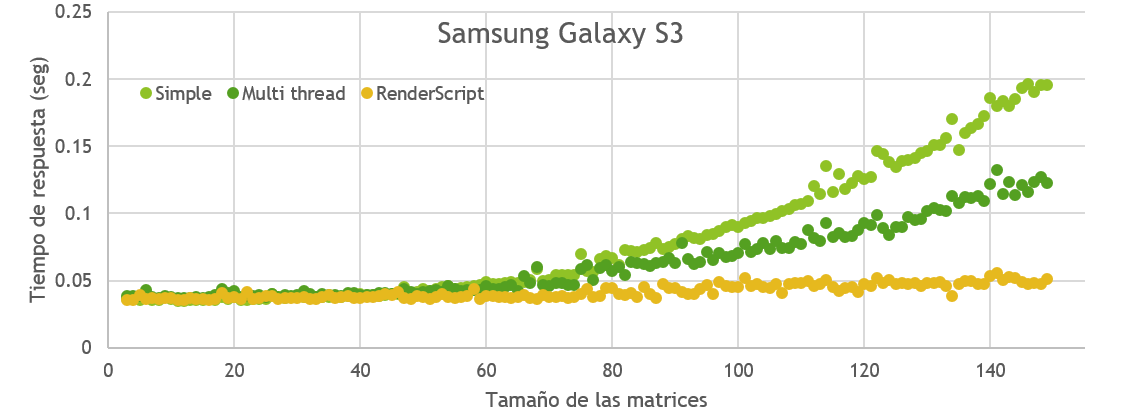
\includegraphics[scale=0.68]{images/Samsung}~
\par\end{centering}

\caption{Mediciones del tiempo de respuesta de los algoritmos de multiplicacion
de matrices\label{fig:Mediciones-del-tiempo-multiplicacion-de-matrices}}
\end{figure}


Respecto a los valores de tiempo registrados, puede notarse que el
tiempo de respuesta de los algoritmos crece polinomialmente respecto
al tamaño de las matrices, lo que coincide con la complejidad temporal
de la multiplicación de matrices que es $O(m\times n\times p)$. También
se observa que la versión del algoritmo multi-thread es mas eficiente
que la versión simple, y la versión usando el framework de RenderScript
es mucho más eficiente que las anteriores debido a la arquitectura
de los procesadores gráficos (GPU), que están diseñados para realizar
operaciones matriciales de coma flotante para el procesamiento de
gráficos y otros calculas.

Lo interesante de este escenario es que permite la creación de modelos
simples, por ejemplo, a partir de la técnica de regresión lineal,
ya que existe una correlación clara entre el tamaño de las instancias
del problema y el tiempo de ejecución que se puede aproximar con la
siguiente expresión:

\begin{center}
$tiempo_{C,D}=constante1+constante2\times m\times n\times p$
\par\end{center}

siendo $tiempo_{C,D}$ es el tiempo estimado de ejecución de un algoritmo
$C$ sobre un dispositivo $D$, para matrices de entrada $A_{m\times n}$
y $B_{n\times p}$.

En el cuadro \ref{tab:caso-de-estudio-1} se contrastan cada una de
las técnicas de regresión con cada uno de los componentes contemplados
en el caso de estudio:

\begin{table}[H]
\begin{doublespace}
\begin{centering}
\resizebox{1\textwidth}{!}{%
\begin{tabular*}{20cm}{@{\extracolsep{\fill}}|l|c|c|c|c|c|c|}
\hline 
 & \multicolumn{2}{c|}{{\large{}Algoritmo simple}} & \multicolumn{2}{c|}{{\large{}Algoritmo multi-thread}} & \multicolumn{2}{c|}{{\large{}Algoritmo RenderScript}}\tabularnewline
\hline 
 & {\large{}CC} & {\large{}RMSE} & {\large{}CC} & {\large{}RMSE} & {\large{}CC} & {\large{}RMSE}\tabularnewline
\hline 
{\large{}Linear Regression} & {\large{}0.9945} & {\large{}0.0042} & {\large{}0.9085} & {\large{}0.0156} & {\large{}0.5718} & {\large{}0.0002}\tabularnewline
\hline 
{\large{}MultiLayer Perceptron} & {\large{}0.9973} & {\large{}0.035} & {\large{}0.9187} & {\large{}0.0148} & {\large{}0.8578} & {\large{}0.013}\tabularnewline
\hline 
{\large{}SGD} & {\large{}0.9945} & {\large{}0.047} & {\large{}0.906} & {\large{}0.0209} & {\large{}0.5122} & {\large{}0.0061}\tabularnewline
\hline 
{\large{}Clusterer} & {\large{}0.996} & {\large{}0.012} & {\large{}0.9903} & {\large{}0.052} & {\large{}09929} & {\large{}0.0003}\tabularnewline
\hline 
\end{tabular*}}
\par\end{centering}
\end{doublespace}

\caption{Resultados obtenidos del primer caso de estudio. \label{tab:caso-de-estudio-1}}
\end{table}


En el cuadro \ref{tab:caso-de-estudio-1} se pueden apreciar las métricas
obtenidas a partir de los modelos calculados. A simple vista, se puede
apreciar que los modelos obtenidos para los dos primeros componentes
presentan una gran correlación, significando que el atributo buscado
(response time) tiene una gran dependencia de los atributos contemplados.
Esto concluye que el tamaño de las matrices multiplicadas influye
en el tiempo de respuesta para obtener el producto de dichas matrices.
En contraste, los modelos obtenidos para el algoritmo RenderScript
no presentan una correlación cercana a 1 como los demás algoritmos.
El componente RenderScript optimiza la ejecución de la multiplicación,
disminuyendo la relación entre el tamaño de la matriz y el tiempo
de respuesta.

En todos los escenarios presentados, se ha optado por el caso intermedio
de adaptación, considerando que el mejor modelo obtenido será aquel
que evite casos de overfitting o underfitting, focalizando el análisis
en los valores de \ac{CC} y \ac{RMSE} intermedios. Por lo tanto,
en este caso, el modelo más eficiente es el\emph{ Multilayer Perceptron.}



\begin{figure}[H]
\begin{centering}
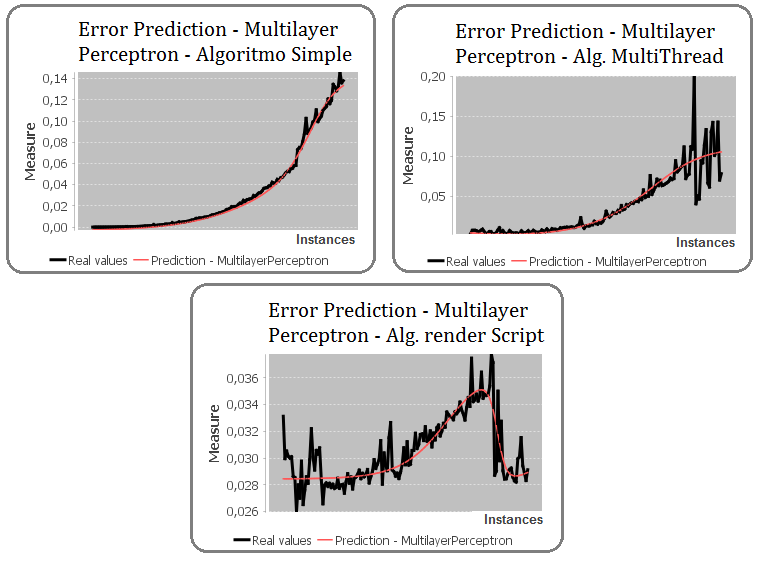
\includegraphics[scale=0.47]{images/response_neural_MM}
\par\end{centering}

\caption{Lineas de predicción en la herramienta Nekonata \label{fig:Lineas-de-predicci=0000F3n-matrix}}
\end{figure}



\section{Caso de estudio 2: algoritmos para el problema del viajante\label{subsec:Escenario-1:-Algoritmos}}

El problema del viajante o \ac{TSP} por sus siglas en inglés es un
problema clásico de optimización combinatoria que consiste en encontrar
la secuencia de caminos de menor distancia que debe recorrer un viajante
para visitar $n$ ciudades una y solo una vez cada una, empezando
por una ciudad cualquiera de ellas y regresando al mismo lugar del
que partió. En el campo de la teoría de complejidad computacional,
el problema del viajante, es un problema NP-Completo y es modelado
como un grafo de manera que las ciudades son sus vértices, los caminos
son las aristas y las distancias entre caminos son los pesos de las
aristas. Es un problema de minimización tras la búsqueda de un recorrido
completo que comienza y finaliza en un vértice específico y visita
el resto de los vértices exactamente una vez con coste mínimo. Existen
muchas variantes del problema, una de ellas se trata del \ac{TSP}
simétrico en el cual la distancia entre un par de ciudades es la misma
en cada dirección formando un grafo ponderado no dirigido. Esta variante
fue la versión considerada por la herramienta. 

Los componentes o algoritmos considerados para este dominio se describen
a continuación: 
\begin{description}
\item [{Best~Fit}] algoritmo heurístico que selecciona las ciudades de
acuerdo al costo de sus trayectos y son incorporadas al conjunto Solución
en base al cálculo de la distancia marginal de las intersecciones.. 
\item [{Nearest~neighbour}] partiendo de alguna ciudad arbitraria se analizan
todos los vértices adyacentes y aún no visitados, y se añade a la
solución aquel vértice cuya arista de costo sea la mínima. 
\item [{Lineal~Programming}] realiza una búsqueda exhaustiva simulando
el algoritmo backtracking, considerando restricciones y funciones
objetivo como fórmulas matemáticas. 
\item [{Prim}] crea un árbol de recubrimiento sobre el grafo y crea un
ciclo euleriano mínimo
\item [{Kruskal}] algoritmo similar a Prim en funcionamiento pero no en
ejecución, variando su complejidad.
\item [{Local~Transformations}] A través de un grafo hamiltoniano, se
analizan las aristas cruzadas obteniendo un nuevo ciclo.
\end{description}
Con el fin de garantizar instancias variadas del problema (diferentes
cantidades de ciudades, distintas representaciones y pesos) y para
la medición de los componentes, se utiliza la librería TSPLib\footnote{https://www.iwr.uni-heidelberg.de/groups/comopt/software/TSPLIB95/}
que contiene archivos con múltiples instancias del problema.. La librería
cuenta con 111 archivos de formato \emph{TSP}. Los ejemplos oscilan
desde 14 y hasta 18512 ciudades con un sólo ejemplo extremo de 85900,
y utilizan cuatro funciones de cálculo de la distancia entre ciudades:
distancia euclidiana, distancia geométrica, distancia pseudo euclidiana
y función techo. Para la obtención de las mediciones correspondientes,
se realizó una pre selección de 32 archivos que comprenden ejemplos
de entre 22 y 200 ciudades. Cabe destacar que fue necesaria la implementación
de un parser para el uso de los archivos. 

Por último, el dataset de mediciones obtenido para el entrenamiento
de modelos incluye atributos de las instancias del problema y propiedades
no-funcionales de la ejecución del componente. Los posibles atributos
de instancia son el número de ciudades, la cantidad de caminos y la
longitud de los mismo, sin embargo sólo se consideró la cantidad de
ciudades; y las propiedades de ejecución del componente son el tiempo
de respuesta, el valor solución, y la exactitud u optimalidad del
resultado, que es la razón entre el valor de la solución encontrada
y el valor óptimo de esa instancia del problema. 

Las pruebas fueron llevadas a cabo sobre los dispositivos móviles
Samsung Galaxy S4, S5 y S6. Los resultados presentados a continuación
consideran el desempeño de los aldoritmos sobre el dispositovo S4
a modo de referencia ya que los mismos no presentaban diferencias
significativas entre sí.

En la figura \ref{tab:response-caso-de-estudio-2-1} se puede observar
el tiempo de respuesta de los diferentes algoritmos considerando la
cantidad de ciudades. A simple vista se puede observar que los algoritmos
aproximados u óptimos tienen menor costo computacional debido que
no exploran la totalidad de ciudades para obtener la respuesta. Mientras
que los algoritmos exactos consumen más tiempo de respuesta ya que
hacen un análisis exhaustivo e incluso pueden requerir de algoritmos
auxiliares como el de ordenamiento. Gráficamente también se puede
observar un umbral en 50 ciudades, dividiendo los tiempos de respuesta
entre los cuales consideran la cantidad de ciudades como un factor
influyente y aquellos en los que pasa desapercibido.

\begin{figure}[H]
\begin{centering}
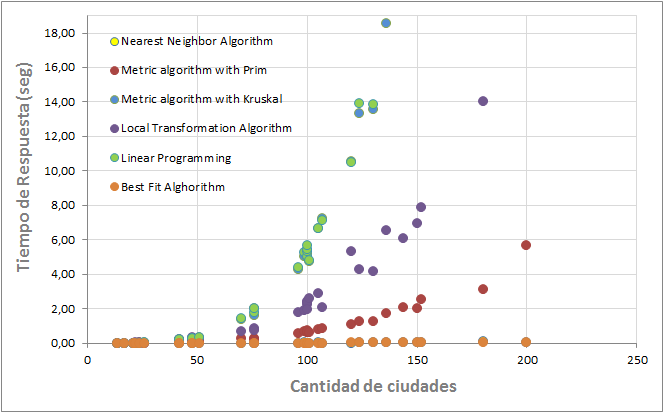
\includegraphics[scale=0.6]{images/S4}
\par\end{centering}

\caption{Mediciones de tiempo de respuesta de los algoritmos de resolución
del problema del viajante. \label{tab:response-caso-de-estudio-2-1}}
\end{figure}


A continuación se presentan los resultados de los modelos de regresión
del tiempo de respuesta:

\begin{table}[H]
\begin{doublespace}
\begin{centering}
\resizebox{1\textwidth}{!}{%
\begin{tabular*}{20cm}{@{\extracolsep{\fill}}|l|c|c|c|c|c|c|}
\hline 
 & \multicolumn{2}{c|}{{\large{}Best Fit}} & \multicolumn{2}{c|}{{\large{}Nearest Neighbour}} & \multicolumn{2}{c|}{{\large{}Linear Programming}}\tabularnewline
\hline 
 & {\large{}CC} & {\large{}RMSE} & {\large{}CC} & {\large{}RMSE} & {\large{}CC} & {\large{}RMSE}\tabularnewline
\hline 
{\large{}Linear Regression} & {\large{}0.98} & {\large{}0.0127} & {\large{}0.9281} & {\large{}0.0191} & {\large{}0.7535} & {\large{}17.8555}\tabularnewline
\hline 
{\large{}MultiLayer Perceptron} & {\large{}0.99} & {\large{}0.0034} & {\large{}0.9806} & {\large{}0.0050} & {\large{}0.9938} & {\large{}10.4876}\tabularnewline
\hline 
{\large{}\ac{SGD}} & {\large{}0.98} & {\large{}0.0045} & {\large{}0.9479} & {\large{}0.0090} & {\large{}0.8522} & {\large{}3.8502}\tabularnewline
\hline 
{\large{}Clusterer} & {\large{}0.98} & {\large{}0.0023} & {\large{}0.9920} & {\large{}0.0024} & {\large{}0.9961} & {\large{}1.5746}\tabularnewline
\hline 
{\large{}\ac{SMO}} & {\large{}0.99} & {\large{}0.0001} & {\large{}0.9999} & {\large{}0.0001} & {\large{}0.9999} & {\large{}0.1214}\tabularnewline
\hline 
\end{tabular*}}
\par\end{centering}
\end{doublespace}

\caption{Resultados obtenidos del caso de estudio dos \label{tab:caso-de-estudio-2}}
\end{table}


\begin{table}[H]
\begin{doublespace}
\begin{centering}
\resizebox{1\textwidth}{!}{%
\begin{tabular*}{20cm}{@{\extracolsep{\fill}}|l|c|c|c|c|c|c|}
\hline 
 & \multicolumn{2}{c|}{{\large{}Prim}} & \multicolumn{2}{c|}{{\large{}Kruskal}} & \multicolumn{2}{c|}{{\large{}Local Transformation}}\tabularnewline
\hline 
 & {\large{}CC} & {\large{}RMSE} & {\large{}CC} & {\large{}RMSE} & {\large{}CC} & {\large{}RMSE}\tabularnewline
\hline 
{\large{}Linear Regression} & {\large{}0.9835} & {\large{}1.1767} & {\large{}0.7553} & {\large{}17.0618} & {\large{}0.8835} & {\large{}4.4046}\tabularnewline
\hline 
{\large{}MultiLayer Perceptron} & {\large{}0.9923} & {\large{}0.1618} & {\large{}0.8993} & {\large{}8.8769} & {\large{}0.9950} & {\large{}0.7954}\tabularnewline
\hline 
{\large{}\ac{SGD}} & {\large{}0.9675} & {\large{}0.3545} & {\large{}0.9941} & {\large{}2.3924} & {\large{}0.9239} & {\large{}2.0863}\tabularnewline
\hline 
{\large{}Clusterer} & {\large{}0.9879} & {\large{}0.1823} & {\large{}0.9926} & {\large{}2.0626} & {\large{}0.9863} & {\large{}0.7248}\tabularnewline
\hline 
{\large{}\ac{SMO}} & {\large{}0.9999} & {\large{}0.0071} & {\large{}0.9999} & {\large{}0.0983} & {\large{}0.9999} & {\large{}0.0242}\tabularnewline
\hline 
\end{tabular*}}
\par\end{centering}
\end{doublespace}

\caption{Resultados obtenidos del caso de estudio dos \label{tab:caso-de-estudio-2-1}}
\end{table}


A partir de los cuadros \ref{tab:caso-de-estudio-2} y \ref{tab:caso-de-estudio-2-1}se
desprenden algunas conclusiones respecto al segundo caso de estudio.
En primer lugar, tanto el modelo de \emph{MultiLayer Perceptron} como
el de \ac{SMO} son, claramente, los mejores en cuanto a adaptación
al modelo. Ambos presentan una correlación de los datos cercano a
1 (\ac{CC}), lo que representa una buena precisión de los datos predichos
en relación a los reales. Como se ha se explicado en la sección\ref{sub:Ajuste-del-modelo:},
esto puede parecer lo más óptimo. Sin embargo, observando las métricas
y las curvas de errores, ambos modelos presentan el problema de overfitting. 

Teniendo esto en cuenta, se descartan las técnicas \emph{MultiLayer
Perceptron y }\ac{SMO} como mejores alternativas para este tipo de
problemas. A su vez, se descarta la técnica \emph{Linear Regression
}ya que presenta los niveles de correlación mas bajos y los errores
más altos.

La técnica que mejor se ajusta para este caso de estudio es el \ac{SGD}.\emph{
}A continuación, se presenta el comportamiento de este último con
respecto a los valores de referencia.

\begin{figure}[H]
\begin{centering}
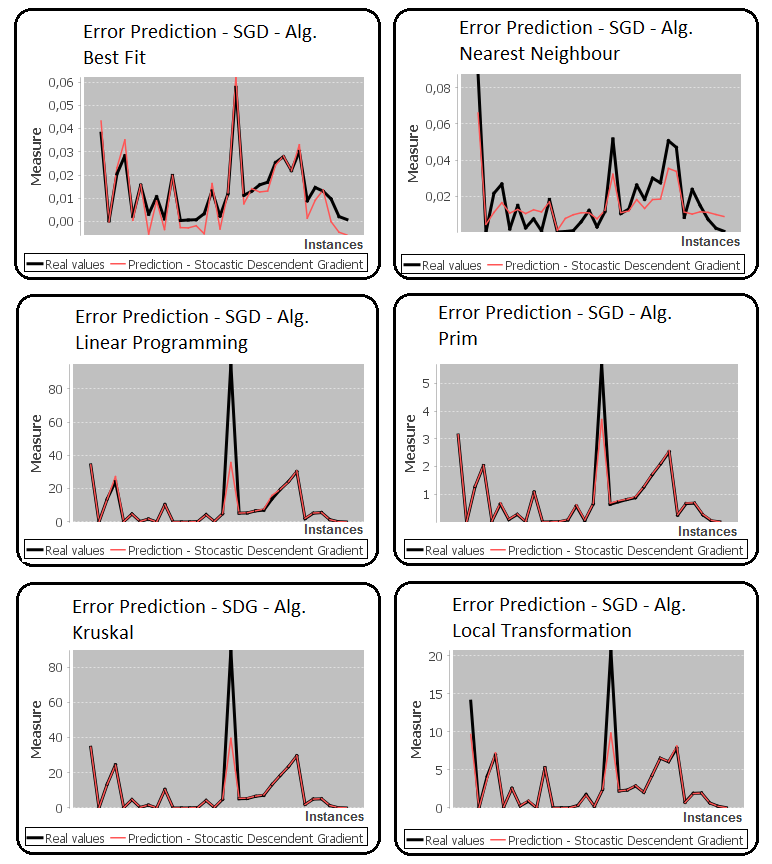
\includegraphics[scale=0.4]{images/response_SGD_TSPLIB}
\par\end{centering}

\caption{Lineas de predicción en la herramienta Nekonata}
\end{figure}



\section{Caso de estudio 3: servicios para detección de rostros\label{subsec:Escenario-2:-Servicios}}

El tercer escenario comprende un conjunto de servicios para la detección
de rostros en imágenes. La función que ofrecen es identificar las
regiones de una imagen que corresponden a rostros humanos. Hoy en
día muchas soluciones para detección de rostro se proporcionan como
servicios Web que, aunque no son tan eficientes y usables sin conexión
a Internet como las bibliotecas de software, resultan generalmente
más precisos y proporcionan características adicionales del rostro
como identificación de sonrisas, género e incluso estimaciones de
edad. Sin embargo, el rendimiento y la precisión de los servicios
varían según las propiedades de la imagen (tamaño, foco, oclusiones)
y contexto de ejecución (capacidad de procesamiento, conexión de red).
En la figura~\ref{fig:Ejemplo-de-detecci=0000F3n}~se muestra un
ejemplo de detección de rostros usando un servicio Web que incluye
identificación de sonrisas y estimación de edad para cada rostro.

\begin{figure}
\begin{centering}
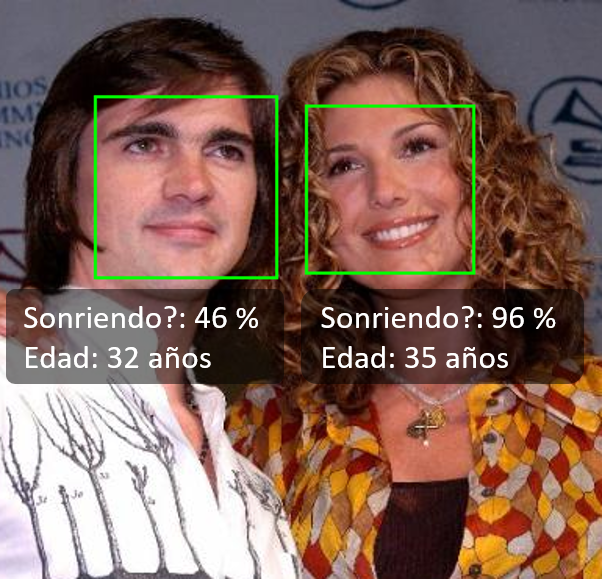
\includegraphics[scale=0.5]{images/ejemplo-de-deteccion-Microsoft-API}
\par\end{centering}

\caption{Ejemplo de detección de rostros en una imagen con el servicio de Microsoft
Face API.\label{fig:Ejemplo-de-detecci=0000F3n}}
\end{figure}


Los componentes considerados en el caso de estudio incluyen un servicio
local para dispositivos Android (Google Play Services face detector\footnote{https://developers.google.com/vision/})
y tres servicios Web (FaceRect API\footnote{http://apicloud.me/apis/facerect},
Sky Biometry API\footnote{https://skybiometry.com} y Microsoft Face
API\footnote{https://azure.microsoft.com/en-us/services/cognitive-services/}). 
\begin{description}
\item [{Google~face~API}] es una API para la detección de rostros en
imágenes y vídeos en tiempo real que forma parte del paquete de servicios
de Google Play para dispositivos Android. Estos servicios proporcionan
una gran variedad de APIs de Google, como geolocalización, servicios
de juegos y algoritmos de visión computacional como detección de rostros.
Al ejecutarse de manera local en el dispositivo, la funcionalidad
de detección de rostros no requiere conexión a Internet.
\item [{FaceRect~API}] es un servicio Web simple y gratuito para detección
de rostros en imágenes, consumido mediante interfaz \ac{REST}. 
\item [{Sky~Biometry~API}] es un servicio Web mas completo que incluye
características adicionales además de detección de rostros. También
es consumido mediante una interfaz \ac{REST}.
\item [{Microsoft~Face~API}] es un servicio Web en la nube que provee
algoritmos de detección y reconocimiento de rostros muy avanzados.
El servicio también se accede a través de una interfaz \ac{REST}.
El servicio forma parte de un grupo de APIs de inteligencia artificial
llamado Servicios Cognitivos.
\end{description}
Estos cuatro componentes fueron evaluados a partir de un subconjunto
de 290 imágenes pertenecientes al dataset llamado FDDB\citep{fddbTechReport}
con características muy variadas, incluyendo imágenes a color y escala
de grises, rostros de diferentes tamaños y posiciones, distintas resoluciones
de imágenes, etc. Como etapa de medición, cada servicio fue llamado
especificando una imagen y un conjunto de parámetros booleanos con
los que se le especifica al servicio que características se desean
extraer de los rostros (posición, sonrisa, edad, etc). Por cada invocación
se mide y registra el tiempo de respuesta en milisegundos. Las mediciones
del servicio Google face API fueron realizadas sobre un dispositivo
Lenovo K3 Note, mientras las mediciones de los servicios Web se realizaron
con la herramienta JMeter\footnote{http://jmeter.apache.org/}.

A diferencia de los casos de estudio anteriores, la correlación entre
el tiempo de respuesta y el tamaño de las instancias (medido, por
ejemplo, como la cantidad de pixeles de la imagen) es muy baja. Esto
se puede observar en la Figura~\ref{fig:Mediciones-del-tiempo-google-face-api},
donde se ilustran las mediciones del tiempo de respuesta para el servicio
de Google respecto al tamaño de las imágenes. Esta correlación es
aun peor es las mediciones de servicios Web, por lo que las propiedades
de las imágenes como su tamaño no fueron consideradas en el dataset
como variables para la predicción. Los atributos del dataset son conformados
por el valor de los parámetros booleanos con los que se invoca el
servicio, lo que conlleva a que existan muchas instancias conformadas
por atributos de igual valor que obtuvieron tiempos de respuestas
distintos.. En consecuencia, dos instancias análogas en sus requerimientos
podrían producir predicciones diferentes lo cual rompe el criterio
de unicidad de toda función matemática.

\begin{figure}
\begin{centering}
\includegraphics[scale=0.7]{\string"images/Google API\string".png}~
\par\end{centering}

\caption{Mediciones del tiempo de respuesta de Google Face API\label{fig:Mediciones-del-tiempo-google-face-api}}
\end{figure}


En el cuadro\ref{tab:caso-de-estudio-3}, se presentan los resultados
de correlación y error de los modelos de tiempo de respuesta obtenidos
para cada servicio:

\begin{table}[H]
\begin{doublespace}
\begin{centering}
\resizebox{1\textwidth}{!}{%
\begin{tabular*}{20cm}{@{\extracolsep{\fill}}|l|c|c|c|c|c|c|c|c|}
\hline 
 & \multicolumn{2}{c|}{{\large{}FaceRect API}} & \multicolumn{2}{c|}{{\large{}SkyBiometry API}} & \multicolumn{2}{c|}{{\large{}Microsoft Face API}} & \multicolumn{2}{c|}{{\large{}Google Face API}}\tabularnewline
\hline 
 & {\large{}CC} & {\large{}RMSE} & {\large{}CC} & {\large{}RMSE} & {\large{}CC} & {\large{}RMSE} & {\large{}CC} & {\large{}RMSE}\tabularnewline
\hline 
{\large{}Linear Regression} & {\large{}0.7000} & {\large{}153.6} & {\large{}0.08} & {\large{}637.54} & {\large{}0.41} & {\large{}71.78} & {\large{}0.6} & {\large{}59.17}\tabularnewline
\hline 
{\large{}MultiLayer Perceptron} & {\large{}0.7} & {\large{}153.52} & {\large{}0.09} & {\large{}637.83} & {\large{}0.58} & {\large{}64.04} & {\large{}0.66} & {\large{}55.54}\tabularnewline
\hline 
{\large{}\ac{SGD}} & {\large{}0.7} & {\large{}704.11} & {\large{}0.06} & {\large{}676.21} & {\large{}0.41} & {\large{}73.3} & {\large{}0.59} & {\large{}59.31}\tabularnewline
\hline 
{\large{}Clusterer} & {\large{}0.991} & {\large{}27.92} & {\large{} 0.13 } & {\large{}633.84} & {\large{} 0.56 } & {\large{}65.28} & {\large{} 0.78 } & {\large{}45.83}\tabularnewline
\hline 
\end{tabular*}}
\par\end{centering}
\end{doublespace}

\caption{Resultados obtenidos del caso de estudio tres. \label{tab:caso-de-estudio-3}}
\end{table}


Los datos exhibidos demuestran que el mejor modelo presentado para
predecir el tiempo de respuesta para el problema de detección de rostros
es el \emph{MultiLayer Perceptron}. El algoritmo no sólo ha arrojado
los valores más bajos del error de predicción sino que en todos los
casos, demuestra una buena adaptación a los dataset que por su naturaleza,
difieren en volumen de instancias, cantidad y tipo de atributos. 

A continuación, se presentan las lineas de predicción para demostrar
el desempeño de la técnica.

\begin{figure}[H]
\begin{raggedright}
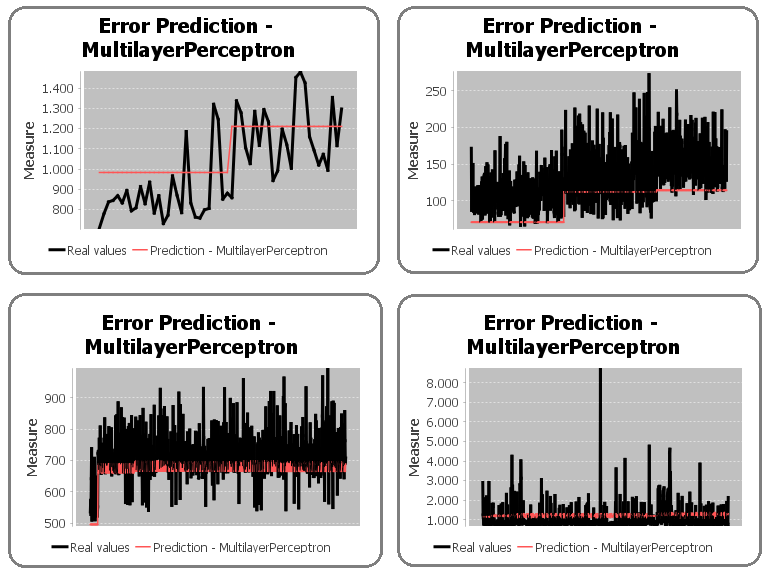
\includegraphics[scale=0.48]{images/response_face_lc}
\par\end{raggedright}

\caption{Lineas de predicción en la herramienta Nekonata \label{fig:Figura-comparativa-de-Multi}}
\end{figure}



\section{Análisis y discusión\label{sec:Analisis-y-discusi=0000F3n}}

En esta sección se analizan y discuten los resultados de las técnicas
entre sí. Es importante mencionar algunas consideraciones sobre la
técnica \ac{SMO} por las cuales se excluyó su aplicación sobre el
segundo y tercer caso de estudio. El desempeño de este algoritmo es
considerablemente superior en la calidad de sus respuestas, sin embargo
presenta algunas limitaciones para su uso; el desempeño del algoritmo
no es apto para formatos de dataset de cientos de instancias y múltiples
atributos, ya que en algunos casos la técnica requirió más de un día
de ejecución y en otros casos, sus resultados no pudieron ser visualizados.

En la evaluación del enfoque sobre los casos de estudio, solo se han
ejecutado los componentes sobre un número reducido de dispositivos.
Por lo tanto, no se consideraron características del dispositivo a
la hora de capturar mediciones y atributos para el entrenamiento de
modelos de predicción. Solo se consideraron atributos de los parámetros
de entrada de los componentes, además de su tiempo de respuesta, por
lo que los modelos solo generalizan la predicción sobre el dispositivo
en los que fueron tomadas las mediciones.

Considerando las mediciones tomadas en la primer etapa, se puede analizar
el comportamiento de los componentes respecto a un conjunto de entradas
particulares. Así, en el primer caso de estudio se puede observar
una gran dependencia entre el tamaño de la las instancias de la entrada
y el tiempo de respuesta. En el segundo caso, esta dependencia se
sigue observando pero mitigada mientras que en el último caso esta
dependencia es baja debido a la complejidad del problema de detección
de rostros. 

Si el desarrollador desea conocer el tiempo de respuesta aproximado
de un componente para un valor de entrada desconocido, utilizará el
modelo de predicción obtenido del aprendizaje. Así, en el primer y
último caso de estudio, el modelo de predicción más conveniente es
el MultiLayer Perceptron, mientras que en el segundo es el \ac{SGD}.
En cuanto a la correlación, se destaca que en el caso de estudio de
multiplicación de matrices, los algoritmos son sencillos y por lo
tanto poseen una correlación muy alta. Esto significa, que la técnica
determinó una buena relación entre las entradas de la función (entradas
del problema) y el atributo a predecir (tiempo de respuesta). En el
segundo caso, esta correlación es más baja debido a la mayor complejidad
del problema del viajante, y por último, en el caso 3, el problema
es más complejo no sólo por su objetivo sino porque no se han encontrado
atributos de las entradas que tengan buena correlacion con el tiempo
de respuesta. Esto significa una correlación mucho más baja y errores
más altos.



Cuanto mayor sea la correlación entre los datos de entrada del problema
y el tiempo de respuesta, menor es el grado de error en la predicción
ya que es más factible que el modelo encuentre una formula matemática
que describa la salida a partir de la entrada.


\section{Conclusiones \label{sec:Conclusiones}}

En este capítulo se presentaron distintos casos de estudio y se analizaron
los resultados producto de los mismos. En la primera sección se describió
el procedimiento llevado a cabo para la evaluación de la calidad de
los modelos predictivos construidos con técnicas de regresión. Luego,
se describieron los escenarios que conforman cada uno de los casos
de estudio donde se aplica el enfoque propuesto con las herramientas
implementadas. Finalmente, se analizan los resultados de los modelos,
de los que se extraen las siguientes consideraciones principales: 
\begin{itemize}
\item En caso de dataset formados por pocas instancias, como el caso de
estudio del problema del viajante, el comportamiento del \ac{SMO}
es similar al del Multilayer Perceptron. Sin embargo, es importante
destacar el efecto de overfit de ambos algoritmos, y particularmente
el tiempo de procesamiento que requiere el \ac{SMO}. 
\item En el caso de un dataset conformado por pocas instancias y buena correlación
entre el tiempo de respuesta y los datos de entrada, , como el caso
de estudio dos, la técnica \ac{SGD} presenta buenos resultados en
el modelo obtenido en relación al tiempo de ejecución que conlleva.
\item Analizando el desempeño de cada técnica y los resultados obtenidos,
se concluye que la mejor técnica para predecir el tiempo de respuesta
ha sido el Multilayer Perceptron. El mismo presenta buenos resultados
en datasets complejos y simples, generalizando el comportamiento de
los datos, como se puede apreciar en las figuras \ref{fig:Figura-comparativa-de-Multi}
y \ref{fig:Lineas-de-predicci=0000F3n-matrix}.\end{itemize}

\acresetall
\chapter{Conclusiones\label{chap:Conclusiones}}

En este trabajo se presentó un modelo de aprendizaje automático para
la estimación de atributos no funcionales en componentes de aplicaciones
Android, un framework de predicción con técnicas de regresión que
permite una gran abstraccióna las implementaciones de bajo nivel de
las librerías de aprendizaje de máquina. Este modelo brinda la posibilidad
de crear modelos predictivos óptimos, adecuados a un conjunto de datos
particular y un atributo a predecir particular.

Ciertamente, el uso de modelos como criterio de calidad para la selección
de servicios y componentes se está extendiendo cada vez más, promoviendo
el desarrollo y optimización de técnicas de aprendizaje de máquina.
En primer lugar, en este trabajo se presentaron las características
principales de las técnicas que aplican aprendizaje sobre los datos,
describiendo en forma detallada los algoritmos y el desafío de optimizar
la configuración de los paramétros. Luego, se estudiaron diferentes
herramientas de recolección de datos en sistemas Android examinando
los principales artefactos y mecanismos involucrados en estas herramientas
y se analizaron dos indicadores principales de performance de componentes,
el tiempo de respuesta y precisión en los resultados. 

Como resultado del creciente desarrollo de aplicaciones, hoy en día,
la integración de componentes de terceros se ha popularizado en diversas
áreas, como por ejemplo la de los dispositivos móviles. En este sentido,
se introdujeron las nociones básicas de los dispositivos móviles,
estudiando también, el sistema operativo más difundido en estos dispositivos,
Android. Se analizaron las características más importantes del mismo,
y se presentaron los conceptos necesarios para comprender el funcionamiento
de las aplicaciones en este sistema.

La utilización de componentes de terceros en dispositivos móviles
presenta ciertos desafíos. Estos dispositivos tienen limitaciones
en conflicto como la energía, el acceso a la red y la capacidad de
cálculo que determinan el contexto de ejecución de estos componentes
y que afecta considerablemente los atributos de calidad de los mismos
y de las aplicaciones que los invocan. Por lo tanto, es importante
elegir los componentes adecuados de acuerdo con su calidad de servicio
además de la funcionalidad requerida. En este sentido se describieron
las investigaciones actuales en el área. Se presentaron los trabajos
que apuntaban a la determinación de relaciones entre las estimaciones
de los atributos de calidad y las propiedades inhatas de los diferentes
dominios o casos de aplicación presentados. 

Por último, se presentaron los experimentos efectuados para validar
el enfoque propuesto. Los mismos fueron evaluados con las métricas
presentadas en secciones anteriores, señalando al modelo MultiLayer
Perceptron como el mejor a nivel de predicciones bajas en error. Las
estimaciones permiten predecir que en dominios de problemas P y NP
como el caso del problema de la multiplicacion de matrices y el problema
del viajante métrico, el nivel de correlación alcanzado por el algoritmo
es inmediatamente inferior al 100\% y en cuanto al error en las predicciones
a través de las métrica \ac{RMSE} , tendrán valores inmediatamente
cercanos o iguales a cero. Para el caso de servicios, aunque las estimaciones
arrojadas por el modelo presentan mas variabilidad, su comportamiento
es considerablemente superior al resto de los modelos, en cuanto evita
efectos de overfit y underfit sobre los datos. Esto indica que una
generalización del modelo propuesto puede resultar útil para determinar
a priori qué componentes resultarán más eficiente, dadas ciertas características
en las entradas, en los componentes y en la operación, tanto para
la predicción del tiempo de respuesta como para la presición.

Por otro lado, las evaluaciones señalan al modelo Linear Regression
como la mejor opción a nivel de generalización en el aprendizaje y
buena adaptación a diferentes formatos de dataset. El factor de correlación
obtenido por este modelo para problemas de complejidad polinómica
alcanza resultados tan precisos como el modelo MultiLayer Perceptron
a un costo computacional extremadamente inferior. Respecto al caso
de estudio de problema NP, el modelo fue capaz de alcanzar valores
de correlacioón entre las variables mayores al 70\%, un valor positivo
teniendo en cuenta un conjunto estrecho de datos de entrenamiento
(cercano a las 200 instancias), y un tiempo de procesamiento reducido
a minutos, tanto para la predicción del tiempo de respuesta como para
la precisión. Incluso, los resultados arrojados fueron superiores
a otras técnicas. Respecto a los servicios, se observa que el modelo
tiene dificultades para aprender, aunque la pobreza de los dataset
formados concentra la mayor responsabilidad. En estos ambientes, el
modelo K means Clusterer logra superar estas dificultades y obtiene
resultados superiores incluso, al modelo MultiLayer Perceptron. Para
el servicio Microsoft conformado por más de 1800 instancias, el modelo
alcanza un factor de correlacion un 2\% menor que el factor determinado
por el modelo MultiLayer Perceptron, y para los servicios Google Play
(2320 instancias) y SkyBiometry (3840 instancias) el modelo de cluster
determina aún mejor la relación entre las variables y reduce el error
en las predicciones respecto al modelo MultiLayer, que por sus resultados
fue tomado como base para el análisis de las técnicas en general. 


\section{Limitaciones}

La principal limitación que presenta el modelo propuesto en este trabajo
parte del problema de la falta de recursos suficientes de los dispositivos
móviles para llevar adelante ejecuciones complejas y costosas, que
insumen gran cantidad de memoria y procesamiento. Este factor, impide
la posibilidad de serializar las primeras dos fases del enfoque propuesto,
obligando a dividir el enfoque en dos herramientas desarrolladas para
ambientes distintos. 

Otra limitación que se presenta responde a la ausencia de un método
automatizado para configurar dinámicamente los parámetros de las tecnicas
de regresión, debiendo determinar un rango estático y específico propio
para cada técnica, para llevar a cabo el proceso de optimización,
considerando de esta forma a todos los datos de entrenamiento por
igual, sin distinción de formato, dominio, etc.

Finalmente, es importante destacar que las estimaciones arrojadas
para los servicios remotos de detección facial, no reflejan conclusiones
claras y determinísticas. Este problema parte de la heterogeneidad
en la formación de los datos, lo que dificulta realizar comparaciones
entre ellos. Por otro lado, no se incoporaron atributos que reflejen
datos reales sobre los rostros en las imágenes ni atributos sobre
los resultados retornados por el servicio, de manera que la precisión
no puede ser analizada, ni contrastada con el tiempo de respuesta
obtenido.


\section{Trabajos Futuros}

Cabe mencionar que existen algunas posibilidades de extensión interesantes
para este trabajo. Como primer objetivo se pretende mejorar el tiempo
de procesamiento requerido para la optimización y generación de los
modelos predictivos. Para poder lograr esto, se le puede otorgar a
la aplicación la capacidad de soportar eficientemente múltiples hilos
de ejecución y distribuir o paralelizar los procesos de optimización
y construcción de los diferentes modelos. Por otro lado, se deben
incoportar dataset con la suficiente expresividad para describir de
mejor manera los diferentes casos de aplicación analizados y derivar
en conclusiones más precisas.

Adicionalmente se pretende incorporar nuevos aspectos para la mejora
y contraste de técnicas. Entre los aspectos a considerar al extender
el proceso de optimización se procura: 
\begin{itemize}
\item Independizar al módulo de optimización de técnicas, de diferentes
rangos de configuración para cada uno de los parámetros que incluya
la técnica. De esta forma, lograr más énfasis en los valores de cada
parámetro y explotar al máximo el desempeño de las técnicas. Incluso,
el usuario podría disponer de la posibilidad de personalizar estos
valores.
\item Informar y registrar el tiempo real consumido por cada operación de
construcción de un modelo. Operación que incluye la configuración,
optimización, entrenamiento y finalmente la construccion del modelo
con la evaluación de las métricas correspondientes. 
\item Extender el análisis comparativo a nivel de librerías, aprovechando
la capacidad de la herramienta de integrar librerías de terceros.
De esta manera, se logra comparar el desempeño de una técnica conocida
en diferentes implementaciones, y seleccionar la mejor técnica independiente
de la librería que la implemente. 
\item Considerar conjuntos de datos de la misma naturaleza que los usados
durante la fase de entrenamiento, para evaluar los modelos creados.
Brindar un mecanismo de evaluación de los modelos a partir de las
métricas, y validar estos modelos creados frente a nuevos conjuntos
de datos para enclarecer el desempeño y generalización lograda. 
\end{itemize}
\selectlanguage{english}%
\selectlanguage{english}%

\acresetall

\selectlanguage{american}%
\newpage{}

\selectlanguage{spanish}%
\bibliographystyle{plainnat}
\addcontentsline{toc}{chapter}{\bibname}\bibliography{Bibliograf-ía}


\newpage{}

\selectlanguage{american}%
\acresetall

\selectlanguage{spanish}%
\appendix

\chapter{Implementación de los algoritmos de resolución de TSP \label{chap:Ambiente-de-desarrollo}}

El Problema del Agente Viajero (\emph{TSP -Travelling salesman Problem})
corresponde a uno de los problemas de optimización más estudiados
de la clase NP-Completos; es un problema de minimización que comienza
y termina en un vértice específico y se visita el resto de los vértices
exactamente una vez. El \ac{TSP} puede ser modelado como un grafo
ponderado no dirigido, de manera que las ciudades sean los vértices
del grafo, los caminos son las aristas y las distancias de los caminos
son los pesos de las aristas.


\section*{Algoritmos de resolución}


\subsection*{1. Best Fit - Bin Packing -}

Best fit es uno de los algoritmos heurísticos más simples,brinda soluciones
óptimas (aproximadas) aunque el algoritmo no asegura el retorno de
la mejor solución. Para dominios de grafos no completos incluso, el
camino solución puede contener arcos con costo infinito (ausencia
de arista). Partiendo del punto \emph{A} se analiza el trayecto más
corto a la siguiente ciudad, sea ésta por ejemplo la ciudad \emph{C},
ambas ciudades se añaden al conjunto Solución: \{A, C, A\} 

En cada paso del algoritmo las ciudades son seleccionadas de acuerdo
al costo de sus trayectos y son incorporadas al conjunto Solución
en base al cálculo de la distancia marginal de las intersecciones. 

La distancia marginal representa la variación en el costo total teniendo
en cuenta el costo directo entre \emph{A} y \emph{C} y el costo del
camino entre \emph{A} y \emph{C} pasando por \emph{B}. (A,B,C). El
par de ciudades \emph{A} y \emph{C} son seleccionadas de forma tal
que hagan mínimo el costo del paso por la ciudad \emph{B}.- 

Ejemplo

\begin{tabular}{|c|c|c|c|c|}
\hline 
\selectlanguage{english}%
\selectlanguage{english}%
 & B & C & D & E\tabularnewline
\hline 
A & 2 & 1 & 10 & 25\tabularnewline
\hline 
B & \selectlanguage{english}%
\selectlanguage{english}%
 & 18 & 5 & 5\tabularnewline
\hline 
C & \selectlanguage{english}%
\selectlanguage{english}%
 & \selectlanguage{english}%
\selectlanguage{english}%
 & 20 & 2\tabularnewline
\hline 
D & \selectlanguage{english}%
\selectlanguage{english}%
 & \selectlanguage{english}%
\selectlanguage{english}%
 & \selectlanguage{english}%
\selectlanguage{english}%
 & 8\tabularnewline
\hline 
\end{tabular}

S: \{ A, C, A\} 

Selección ciudad E: 

Trayectos: AC - CA

En tal caso, los trayectos son análogos como así también la distancia
marginal: E se añade entre las ciudades C y A. 

S: \{ A,C,E,A\} 

Costo: 28 

En el siguiente paso la ciudad B es seleccionada: 
\begin{lyxlist}{00.00.0000}
\item [{Trayectos:}]~

\begin{lyxlist}{00.00.0000}
\item [{$AC:D=costo(A,B)+costo(B,C)-costo(A,C)=19$}]~
\item [{Resultando}] S: \{A, B, C, E, A\} Costo ahora:28+19=47 
\item [{\,}]~
\item [{$CE:D=costo(C,B)+costo(B,E)-costo(C,E)=21$}]~
\item [{Resultando}] S: \{A, C, B, E, A\} Costo ahora:28+21=49
\item [{\,}]~
\item [{$EA:D=costo(E,B)+costo(B,A)-costo(E,A)=-18$}]~
\item [{Resultando}] S: \{A, C, E, B, A\} Costo ahora:28-18=10
\end{lyxlist}
\end{lyxlist}
B es añadida entre las ciudades del trayecto cuya distancia es menor,
en el ejemplo ilustrado, la opción del tercer trayecto.


\subsection*{2. Vecino más cercano}

Partiendo de alguna ciudad arbitraria se analizan todos los vértices
adyacentes y aún no visitados, y se añade a la solución aquel vértice
cuya arista de costo sea la mínima. Tal análisis prosigue a partir
del último vértice añadido hasta haber visitado todas las ciudades. 

A menudo, el \ac{TSP} sigue un modelo de grafo completo donde cada
par de vértices es conectado por una arista, en tal caso el algoritmo
brinda soluciones óptimas partiendo desde y hacia la ciudad inicial
pasando exactamente una vez por cada ciudad restante. 

Por otro lado,en modelos donde no existe camino entre algunos pares
de ciudades, la elección iterativa de la arista de mínimo costo sin
una vista global del modelo, puede apartar vértices de la solución
retornando soluciones parciales. 

Ejemplo

\includegraphics{\string"C:/Users/usuario/Desktop/Tesis rubbish/tesis/images/TPS-graph-example\string".png}

Solución: A -> B -> C -> D -> A 

Costo: 97


\subsection*{3. Programación Lineal}

El \ac{TSP} puede ser formulado de manera teórica mediante una (o
varias) formulaciones lineales enteras usando programación lineal
en enteros. Se plantean las variables del problema: 

\begin{lstlisting}[basicstyle={\footnotesize},breaklines=true,language=Java,captionpos=t,tabsize=3,frame=no,keywordstyle={\color{blue}},commentstyle={\color{gray}},stringstyle={\color{red}},numbers=left,numberstyle={\tiny},numbersep=5pt,breaklines=true,showstringspaces=false,basicstyle={\footnotesize},emph={label}]
vértices: 0.. n 	
Xij = 1 | Xij = 0 //para i,j = 0...n
La arista (i,j) pertenece(1)/ no pertenece (0) al conjunto solución.
Cij Distancia desde la ciudad i hasta j //para i,j = 0...n	 
aristas número total de aristas. 	
aristasReq número mínimo de aristas para solución. 
\end{lstlisting}



\subsection*{4. Backtracking}

Backtracking es un algoritmo general para encontrar todas o algunas
soluciones para problemas computacionales con notables restricciones
de satisfacción para dicho problema.El método de búsqueda es incremental
de los candidatos a la solución, abandonando aquellos (\emph{backtrackeando})
tan pronto como se determina que dicha solución no es o va a ser válida. 

En el caso del \ac{TSP}, los posibles candidatos a la solución se
determinan mediante el grado de incidencia de todos los nodos que
componen el grafo. Ya que la ciudad sólo debe ser visitada una vez,
el grado de incidencia de cada ciudad debe ser igual a 2, por lo que
aquellas ciudades que no han sido visitadas (grado de incidencia 0)
o aquellas que sólo han sido destino (grado de incidencia 1) son candidatas
a componer la solución.

Pseudo-código: 

\begin{lstlisting}[language=Java,numbers=left,numberstyle={\tiny},basicstyle={\footnotesize},breaklines=true,captionpos=t,frame=no,keywordstyle={\color{blue}},commentstyle={\color{gray}},stringstyle={\color{red}},numbersep=5pt,emph={label}]
backtracking(costoAct, minCost, lastV, currPath, bestPath, costoAct) 
si costoAct<minCost //Poda por costo que se arrastra 	
	si !solucion(currPath) 		
		generarAristasFactibles(lastV) 		
		Por v:AristasFactibles 			
			costoAct+=v.costo; 			
			currPath= currPath + {v}; 			
			backtracking(costoAct, minCost, v.Destine, currPath); 			
			costoAct-=v.costo; 			
			currPath=currPath - {v}; 	
	sino 		
		bestPath=currPath; //Setear la solución ya encontrada 		
		minCost=costoAct;
\end{lstlisting}



\subsection*{TSP simétrico }

El TSP simétrico es una variedad del problema TSP que para todas las
aristas se cumple la desigualdad triangular o de Minkowski: 

\[
(a,c)<(a,b)+(b,c)
\]


Considerando que no todos los grafos creados cumplen con dicha condición,
y que aún así hay que devolver un resultado óptimo, se considera prioridad
la distancia entre los nodos y no si los mismos se repiten o no.


\subsubsection*{4. Árbol de recubrimiento }

Para resolver el \emph{Metric TSP}, se puede utilizar el método de
árbol de recubrimiento mínimo. El mismo se puede obtener mediante
Prim o Kruskal para, luego de eso, nos aseguramos que el grafo será
simétrico mediante la duplicación de cada arista. Gracias a esto,
podemos recorrerlo mediante un algoritmo recursivo y obtenemos el
ciclo euleriano del mismo. Para finalizar la resolución y mediante
la desigualdad antes planteada, se omiten los nodos repetidos, obteniendo
el ciclo hamiltoniano.


\subsubsection*{4.1 Prim}

El algoritmo Prim toma un tomar un vértice arbitrario de los ya visitados
y lo une con el vértice no visitado mediante el menor arco que salga
de él.

Pseudocódigo:

\begin{lstlisting}[language=Java,numbers=left,numberstyle={\tiny},basicstyle={\footnotesize},breaklines=true,captionpos=t,frame=no,keywordstyle={\color{blue}},commentstyle={\color{gray}},stringstyle={\color{red}},numbersep=5pt,emph={label}]
Prim(firstCity){ 	
	visited={firstCity}; 	
	while (visited!=allCities){ 		
		edge=obtenerMinEdge(visited); 		
		sol= sol ∪ {edge}; 		
		visited= visited  ∪ {edge.destino};
	} 	
return sol; }
\end{lstlisting}



\subsubsection*{4.2 Kruskal}

Kruskal mientras tanto tiene ordenados las aristas por costo y va
agregando a la solución aquellos que ya han sido visitados con los
que no.

Pseudocódigo:

\begin{lstlisting}[language=Java,numbers=left,numberstyle={\tiny},basicstyle={\footnotesize},breaklines=true,captionpos=t,frame=no,keywordstyle={\color{blue}},commentstyle={\color{gray}},stringstyle={\color{red}},numbersep=5pt,emph={label}]
Kruskal(firstCity){ 	
	visited={firstCity}; 	
	edges=getSortedEdges(); 	
	∀ e ∈ edges{ 		
		if (e ∈ (visited)x(not_visited)) 			
			sol=sol ∪ {e}; 			
			visited=visited ∪ {e.destino} 		
	} 
	return sol; }
\end{lstlisting}


La única diferencia entre ambos algoritmos de recubrimiento es la
forma de trabajo de los mismos y en consecuencia su complejidad.


\subsubsection*{4.3 Transformaciones Lineales}

Las transformaciones locales se utilizan para mejorar el hamiltoniano
obtenido por los algoritmos antes presentados. Para introducir el
algoritmo, consideremos la siguiente situación:

\includegraphics{\string"C:/Users/usuario/Desktop/Tesis rubbish/tesis/images/TPS-local-transformations\string".png}

Los nodos unidos en el ciclo hamiltoniano son (A,B) ... (C,D) - línea
no punteada en el grafo. 

Ahora bien, para aplicar transformaciones locales se debe verificar: 

\[
(A,C)+(B,D)<(A,B)+(C,D)
\]


De suceder esto, se pueden modificar los arcos y obtener:

\includegraphics{\string"C:/Users/usuario/Desktop/Tesis rubbish/tesis/images/TPS-local-transformations2\string".png}

El resultado es un grafo con menor costo que el anterior presentado.

\chapter{Descripci�n de los servicios de detecci�n facial \label{chap:Ambiente-de-desarrollo}}


\section*{Servicio SkyBiometry}


\subsection*{En referencia al uso de la API \textendash{} Autenticaci�n }

Cada llamada a la API debe ser autorizada mediante el uso de dos claves:
api\_key y api\_secret. Ambas claves son obtenidas mediante una registraci�n
en el sitio oficial de skybiometry (\emph{www.skybiometry.com}) a
trav�s de una cuenta de email como usuario y una contrase�a.


\subsection*{L�mites de uso }

El consumo de este servicio presenta algunas limitaciones que var�an
en base a la suscripci�n particular del usuario. En general, las suscripciones
gratuitas restringen un l�mite de 100 llamadas a m�todos por hora
y de 5000 en el mes. Para el caso del m�todo POST, la limitaci�n se
presenta tanto en 100 request a la API para el procesamiento de im�genes
individuales como para 1 request con 100 im�genes a procesar. 


\subsection*{Factores ofrecidos}
\begin{lyxlist}{00.00.0000}
\item [{Respecto~al~cuadrado~del~rostro~detectado:}]~

\begin{lyxlist}{00.00.0000}
\item [{center~OBJECT~\{~x~:Float,~y~:~Float~\}}]~
\item [{width.~FLOAT.~0-100\%~del~ancho~del~rostro~respecto~al~ancho~de~la~imagen.}]~
\item [{height.~FLOAT.~0-100\%~del~largo~del~rostro~respecto~al~ancho~de~la~imagen.}]~
\end{lyxlist}
\item [{Otros~puntos~detectados:}]~

\begin{lyxlist}{00.00.0000}
\item [{mouth\_center}] OBJECT \{ x :Float, y : Float \} 
\item [{mouth\_left}] OBJECT \{ x :Float, y : Float \}
\item [{mouth\_right}] OBJECT \{ x :Float, y : Float \} 
\item [{eye\_left}] OBJECT \{ x :Float, y : Float \} 
\item [{eye\_right}] OBJECT \{ x :Float, y : Float \} 
\item [{nose}] OBJECT \{ x :Float, y : Float \} 
\item [{ear\_left}] OBJECT \{ x :Float, y : Float \} 
\item [{ear\_right}] OBJECT \{ x :Float, y : Float \} 
\item [{chin}] OBJECT \{ x :Float, y : Float \} 
\item [{yaw.}] FLOAT.Perfil. Value -90\textdegree{} a 90\textdegree{} 
\item [{roll.}] FLOAT. �ngulo de rotaci�n del rostro. Value -90\textdegree{}
a 90\textdegree{} 
\item [{pitch.}] FLOAT. Value -90\textdegree{} a 90\textdegree{} 
\end{lyxlist}
\end{lyxlist}
\begin{description}
\item [{yaw:}] �ngulo positivo en rostros donde predomina el perfil derecho
(respecto al sujeto, no a la imagen). Caso contrario, �ngulo negativo
al predominar el perfil izquierdo. 
\item [{Roll:}] Ejemplo ilustrativo. El rect�ngulo verde representa al
rostro detectado por la API cuyo valor roll es igual a -17\textdegree ,
mientras que el rect�ngulo rojo fue a�adido para ilustrar el caso
donde el �ngulo roll es igual a 0\textdegree . Una rotaci�n inversa
significa un valor roll positivo. 
\item [{\includegraphics{\string"C:/Users/usuario/Desktop/Tesis rubbish/tesis/images/face-example\string".png}}]~
\end{description}
Todos los puntos detectados descritos no especificados corresponden
a un formato JSON, cuya clave es el nombre del mismo, y el valor es
tambi�n un objeto del tipo JSON que contiene los siguientes valores:
id:INTEGER, confidence:INTEGER, y:FLOAT, x:FLOAT, a excepci�n del
valor \emph{center} cuyo objeto JSON contiene s�lo los valores: \emph{x},
\emph{y}.
\begin{description}
\item [{Nota1:}] en caso de valor de atributo no se puede determinar que
no se devuelve. Si se determina el valor que se devuelve junto con
el valor de confianza como porcentaje de 0 a 100. 
\item [{Nota2:}] La API s�lo devuelve informaci�n necesaria para representar
en forma de rect�ngulo los rostros detectados. Para el resto de opciones,
la API s�lo devuelve informaci�n del punto central en cuesti�n. 
\item [{Nota3:}] Ya que la API autom�ticamente re-escala las im�genes a
1024 pixeles para su procesamiento interno, todas las coordenadas
son provistas de forma porcentual respecto al ancho y largo de la
imagen (abstracci�n). 
\item [{Nota4:}] Nota: el atributo face es el valor por defecto y siempre
es retornado, independientemente de los atributos especificados. Si
el atributo \textquotedblleft glasses\textquotedblright{} fue requerido
adicionalmente se retorna el atributo \textquoteleft dark\_glasses\textquoteright{}
para diferenciar entre gafas oscuras y claras. El atributo mood (estado
de �nimo) se devuelve junto con 7 m�s atributos: confianza para cada
una de las emociones b�sicas, adem�s de la confianza neutral\_mood. 
\end{description}

\subsection*{Atributos faciales }

The result of the API call is a JSON or XML object containing the
requested information. Cada uno de los atributos son objetos del tipo
JSON cuya clave es el nombre del mismo y el valor es tambi�n un objeto
JSON con dos valores espec�ficos: el primero con clave \emph{value}
y el segundo con clave \emph{confidence}. El valor de confidence es
del tipo Integer para representar el porcentaje de probabilidad del
valor detectado en el campo \emph{value}.


\subsection*{Mensajes de error }

\includegraphics[scale=0.55]{\string"C:/Users/usuario/Desktop/Tesis rubbish/tesis/images/face-service-errors\string".png}


\subsection*{Post (Request en lenguaje JAVA)}

\begin{lstlisting}[language=Java,breaklines=true]
HttpResponse<JsonNode> response = Unirest.post(https://face.p.mashape.com/faces/detect?api_key=[api_key]&api_secret=[api_secret]) 
.header(X-Mashape-Key, 7rS5YDw5YHmshtdgMHP2ZYBLAljfp1OxKNzjsn1GJxNBgad6C9) 
.header(Accept, application/json) 
.field(attributes, all) 
.field(detector, Aggressive)  [ver opciones] 
.asJson();        
\end{lstlisting}

\begin{description}
\item [{Nota:}] En los espacios {[}api\_key{]} y {[}api\_secret{]} deben
colocarse las claves correspondientes disponibles con la registraci�n
de una cuenta en el sitio www.skybiometry.com \end{description}
\begin{lyxlist}{00.00.0000}
\item [{Opciones:}]~

\begin{lyxlist}{00.00.0000}
\item [{.field(\textquotedblleft files\textquotedblright ,}] Vector<File>
imagenes) 
\item [{.field(\textquotedblleft files\textquotedblright ,}] File imagen) 
\item [{.field(\textquotedblleft urls\textquotedblright ,}] \textquotedblleft \textquotedblright url\_1\textquotedblright ,
\textquotedblleft url\_2\textquotedblright , \dots ) 
\end{lyxlist}
\end{lyxlist}
\begin{description}
\item [{Nota:}] Los formatos de imagen aceptados por la API son los siguientes:
PNG, JPEG, BMP, JPEG2000.
\end{description}
La respuesta recibida por el servicio del tipo HttpResponse<JsonNode>
puede ser manipulada como un objeto del tipo JSONObject a trav�s de
la siguiente codificaci�n: 

\begin{lstlisting}[language=Java,breaklines=true]
JSONObject obj = response.getBody().getObject(); 
\end{lstlisting}



\subsection*{Parse - Overview }

La respuesta en formato JSONObject contiene en primera parte un objeto
del tipo JSONObject con clave \emph{photos} y cuyo valor, representado
en formato JSONArray, contiene toda la informaci�n detectada desde
las im�genes. Cada elemento del arreglo representa un archivo de imagen;
a su vez, estos elementos contienen un objeto del tipo JSONObject
cuya clave es \emph{tags} y su valor es un JSONArray para representar
cada una de los rostros detectados en la imagen particular; a su vez
contiene la informaci�n de ancho y largo asociado. 

En segunda parte, seguido de \emph{photos} se anexan en la respuesta
la informaci�n relacionada a la operaci�n http.

Ejemplo codificaci�n b�sica: 

\begin{lstlisting}[language=Java,breaklines=true]
JSONArray im�genes = obj.get(photos); 
for(int p=0; p<im�genes.length(); p++) { 
	//Obtenci�n de cada una de las im�genes  	
	JSONObject imagen=imagenes.getJSONObject(p);   
	//Ejemplo obtenci�n del ancho de la imagen 
	int imgWidth = (int) imagen.get(width); 
	//Obtenci�n de los rostros detectados en la imagen 
	JSONArray rostros = imagen.getJSONArray(tags); 
	for(int r=0; r<rostros.lenght(); r++) { 
		//Obtenci�n de cada uno de los rostros detectados 
		rostro=rostros.getJSONObject(r);     	 
		//Ejemplo obtenci�n de los puntos detectados JSONObject 
		mouth = rostro.getJSONObject(mouth_center); 
		int coordX= (int) mouth.get(x); 
		int coordY= (int) mouth.get(y); 
		//Ejemplo obtenci�n de los atributos faciales JSONObject 
		atributos=imagen.getJSONObject(attributes); 
		String valor = atributos.getJSONObject(mood).getString(value); 
	} 	
} 
\end{lstlisting}



\section*{Servicio FaceRect}


\subsection*{En referencia al uso de la API }

El consumo de esta API requiere la registraci�n de una cuenta en el
sitio Mashape. La registraci�n se realiza con email y contrase�a y
se realiza de manera gratuita e instant�nea. El servicio no restringe
el n�mero de request a la API pero permite el procesamiento de s�lo
una imagen por request realizado. 


\subsection*{Factores ofrecidos }
\begin{lyxlist}{00.00.0000}
\item [{Rostro~detectado:}]~

\begin{lyxlist}{00.00.0000}
\item [{Orientation:}] tipo String. Valores posibles:<frontal, profile-right,
profile-left> 
\item [{x:}] tipo Integer 
\item [{y:}] tipo Integer 
\item [{width:}] tipo Integer 
\item [{height:}] tipo Integer 
\item [{Features:}] (opcional) 
\item [{eyes}]~
\item [{nose}]~
\item [{mouth}]~
\end{lyxlist}
\end{lyxlist}
Los \emph{features} son analizados por la API s�lo en rostros cuya
orientaci�n sea frontal. El formato de respuesta de los mismos son
del tipo JSONObject en el caso de \emph{nose} y \emph{mouth}. Para
el caso de \emph{eyes} se devuelve un objeto del tipo JSONArray, cuyos
elementos (1 o 2) son del tipo JSONObject. La API representa el rostro
y los features detectados en forma de rect�ngulos, por lo que incorpora
en sus respuestas las coordenadas \emph{x}, \emph{y} (esquina superior
izquierda respecto a la imagen) y los tama�os \emph{width}, \emph{height}
del rect�ngulo en cuesti�n.


\subsection*{Post (Request en lenguaje JAVA)}

\lstinline[language=Java,breaklines=true]!HttpResponse<JsonNode> response = Unirest.post(ENDPOINT) .header(X-Mashape-Key, 7rS5YDw5YHmshtdgMHP2ZYBLAljfp1OxKNzjsn1GJxNBgad6C9) [ver opci�n correspondiente] .field(features, true) .asJson();        !

Actualmente la API soporta dos endpoints difiriendo entre s� en el
modo en que las im�genes son especificadas en el request. Mediante
el m�todo http \emph{GET} se a�ade el URL de la imagen (Endpoint:
http://apicloud-facerect.p.mashape.com/process-url.json); por otra
parte con el m�todo \emph{POST} se a�ade el archivo correspondiente
(Endpoint: http://apicloud-facerect.p.mashape.com/process-file.json)
De acuerdo con el endpoint especificado se a�ade la l�nea correspondiente: 
\begin{lyxlist}{00.00.0000}
\item [{Opciones}]~

\begin{lyxlist}{00.00.0000}
\item [{.field(\textquotedblleft url\textquotedblright ,}] \textquotedblleft url\_image\textquotedblright ) 
\item [{.field(image,}] new File(<path\_image>)) 
\end{lyxlist}
\end{lyxlist}
\begin{description}
\item [{Nota:}] Para ambos casos, la API restringe el procesamiento de
algunas im�genes, permitiendo procesar aquellas cuyo formato sea JPEG,
PNG y GIF, la resoluci�n de la misma no supere los 4096 p�xeles (4096\texttimes 4096)
y el tama�o sea inferior a 10 MBytes. 
\end{description}
La respuesta recibida por el servicio del tipo HttpResponse<JsonNode>
puede ser manipulada como un objeto del tipo JSONObject a trav�s de
la siguiente codificaci�n: 

\begin{lstlisting}[language=Java,breaklines=true]
JSONObject obj = response.getBody().getObject();
\end{lstlisting}



\subsection*{Parse - overview}

La respuesta en formato JSONObject contiene dos objetos JSON. El primero,
cuya clave es \emph{faces} contiene toda la informaci�n detectada
desde la imagen, el segundo objeto cuya clave es \emph{image} contiene
la informaci�n acerca del ancho (\emph{width}) y largo (\emph{height})
de la misma. La informaci�n detectada se presenta en un objeto del
tipo JSONArray donde cada elemento del arreglo constituye cada uno
de los rostros que ha detectada la API; Cada uno de los elementos
son JSONObject que contienen la informaci�n del rostro (\emph{orientation},
\emph{x}, \emph{y}, \emph{height}, \emph{width}) y los \emph{features}. 

Ejemplo codificaci�n b�sica 

\begin{lstlisting}[language=Java,breaklines=true]
//Ejemplo obtenci�n del ancho de la imagen 
int imgWidth = (int) obj.getJSONObject(image).get(width); 
//Obtenci�n de los rostros detectados en la imagen 
JSONArray rostros = obj.getJSONArray(faces); 
for(int r=0; r<rostros.lenght(); r++) {  	
	//Obtenci�n de cada uno de los rostros detectados 
	rostro=rostros.getJSONObject(r);     	 
	//Ejemplo obtenci�n informaci�n del rostro: 
	String orientation =(String) rostro.get(orientation); 
	int coordX=(int) rostro.get(x); 
	//Ejemplo obtenci�n de los features 
	JSONObject features = rostro.getJSONObject(features); 
	JSONArray eyes =features.getJSONArray(eyes); 
	JSONObject eye_left=eyes.getJSONObject(0); 
}
\end{lstlisting}



\section*{Servicio GMS Vision}


\subsection*{Factores ofrecidos}

El detector puede computar los siguientes atributos (accesibles a
trav�s de los distintos m�todos de la clase).

Profile: rotaci�n del rostro. FLOAT 
\begin{lyxlist}{00.00.0000}
\item [{Clasificadores:<caracter�stica~facial~presente~en~el~rostro>}]~

\begin{lyxlist}{00.00.0000}
\item [{Open}] eyes: (probabilidad) Constant value: 1 FLOAT ({*}) 
\item [{Smiling:}] (probabilidad) Constant value: 1 FLOAT ({*}) 
\item [{Height,}] width: medidos en p�xeles. FLOAT 
\item [{Position:}] Punto superior izquierdo del rostro. FLOAT 
\end{lyxlist}
\item [{Landmarks:<Puntos~de~inter�s~en~el~rostro~detectado>~LIST<Landmark>}]~

\begin{lyxlist}{00.00.0000}
\item [{BOTTOM\_MOUTH}] Constant Value: 0 CENTER 
\item [{LEFT\_CHEEK}] Constant Value: 1 CENTER 
\item [{LEFT\_EAR\_TIP}] Constant Value: 2 
\item [{LEFT\_EAR}] Constant Value: 3
\item [{MIDPOINT}] LEFT\_EYE Constant Value: 4 
\item [{CENTER}] LEFT\_MOUTH Constant Value: 5 
\item [{NOSE\_BASE}] Constant Value: 6 
\item [{MIDPOINT}] RIGHT\_CHEEK Constant Value: 7 
\item [{CENTER}] RIGHT\_EAR\_TIP Constant Value: 8 
\item [{RIGHT\_EAR}] Constant Value: 9 
\item [{MIDPOINT}] RIGHT\_EYE Constant Value: 10 
\item [{CENTER}] RIGHT\_MOUTH Constant Value: 11 
\end{lyxlist}
\item [{Angles:~<Face~Orientation>}]~

\begin{lyxlist}{00.00.0000}
\item [{EulerY}] {[}valor \textquoteleft y\textquoteright{} en la imagen{]} 
\item [{EulerZ}] {[}valor \textquoteleft r\textquoteright{} en la imagen{]}
\end{lyxlist}
\item [{({*})}] En el trabajo desarrollado se consider� el uso de valores
booleanos, determinando a los clasificadores como verdaderos para
valores de probabilidad mayor al 50\%, en casos contrario se determinaron
los mismos como falsos. \end{lyxlist}
\begin{description}
\item [{Nota:}] El �ngulo EulerZ se encuentra disponible siempre en la
detecci�n, mientras que el �ngulo EulerY s�lo si en el detector se
predetermina el modo \emph{accurate}. El concepto de \emph{left} y
\emph{right} son relativos al sujeto no a la posici�n cuando se observa
la imagen. Las posiciones son accedidas a trav�s del m�todo getPosition()
de la clase Landmark; el retorno es del tipo PointF. 
\end{description}

\subsection*{Construcci�n del detector }

\begin{lstlisting}[language=Java,breaklines=true]
FaceDetector detector = new FaceDetector.Builder(context) 
.setTrackingEnabled(false) 
.setMode(int Mode) 
.setProminentFaceOnly(true) 
.setClassificationType(int classificationType) 
.setLandmarkType(int landmarkType) 
.build(); 
\end{lstlisting}


Es necesario especificar en el detector el entorno de nuestra aplicaci�n
(mediante el uso de la clase android.utils.Context) 

Es posible obtener el entorno de la app a trav�s del m�todo \emph{getApplicationContext()}
de la clase Activity. 

El contexto es s�lo una interfaz cuya implementaci�n est� prevista
por el sistema android y permite el acceso a los recursos y clases
espec�ficas de la aplicaci�n, como as� tambi�n realizar operaciones
tales como el despacho de actividades, la difusi�n y recibimiento
de objetos del tipo Intent, etc. 

El servicio dispone de la posibilidad de elegir la preferencia de
procesamiento en la detecci�n, \emph{FAST\_MODE} prioriza la rapidez
en el an�lisis por sobre la cantidad de rostros detectados y su precisi�n,
contrariamente el servicio dispone del modo \emph{ACCURATE\_MODE}

Habilitar la opci�n \emph{tracking enabled} es recomendable para la
detecci�n de im�genes individuales no relacionadas (a diferencia de
un v�deo o una serie de im�genes fijas capturadas consecutivamente). 

Tanto los clasificadores y landmarks pueden especificarse uno a uno
a�adiendo las l�neas correspondientes en el constructor; adicionalmente
la clase FaceDetector proporciona las siguientes constantes: 
\begin{lyxlist}{00.00.0000}
\item [{\emph{ALL\_CLASSIFICATIONS}}]~
\item [{\emph{ALL\_LANDMARKS}}]~
\item [{\emph{NO\_CLASSIFICATIONS}}]~
\item [{\emph{NO\_LANDMARKS}}]~
\end{lyxlist}
El servicio no ofrece la capacidad de setar los landmark y clasificadores
bajo demanda, sino que son definidos est�ticamente al momento de crear
el detector; esta restricci�n condiciona el tiempo de respuesta del
servicio ya que el requerimiento de al menos un landmark, por ejemplo,
significa el uso de la variable \emph{FaceDetector.ALL\_LANDMARKS},
incrementando as� el tiempo de procesamiento de la imagen. 


\subsection*{Uso del detector}

El detector se puede llamar de forma sincronizada con un objeto del
tipo Frame para detectar las caras.

\begin{lstlisting}[language=Java,breaklines=true]
Frame frame = new Frame.Builder().setBitmap(<file_image>).build(); 
SparseArray<Face> faces = detector.detect(frame); 
\end{lstlisting}



\subsection*{Ejemplo codificaci�n b�sica}

\begin{lstlisting}[language=Java,breaklines=true]
for(int i=0;i<faces.size();i++){ 
	//Obtenci�n de cada uno de los rostros detectados en la imagen 
	Face rostro=faces.valueAt(i); 
	//Obtenci�n del rect�ngulo del rostro 
	Float coordX=rostro.getPosition().x; 
	Float coordY=rostro.getPosition().y; 
	Float width=rostro.getWidth(); 
	Float height=rostro.getHeight(); 
	//Obtenci�n del �ngulo EulerZ 
	Float angleZ=rostro.getEulerZ(); 
	//Obtenci�n del clasificador eyes open 
	Float probEyeRight=rostro.getIsRightEyeOpenProbability(); 
	Float probEyeLeft=rostro.getIsLeftEyeOpenProbability(); 
	//Obtenci�n de los Landmarks detectados: 
	List<Landmark> landmarks=rostro.getLandmarks(); 	 
	//Obtenci�n de cada uno de los landmark 
	for(int j=0;j<landmarks.size();j++){ 
		int LandmarkType=landmarks.get(j).getType(); 
		PointF Landmarkposition=landmarks.get(j).getPosition(); 
	} 
} 
\end{lstlisting}

\selectlanguage{english}%

\end{document}
